\chapter{\label{cnn} Machine learning for continuous wave searches}
%%%%%%%%%%
%%%%%%%%%%

%--------------------------
% Introduce machine learning
%----------------------------

Machine learning is a term which was used by Arthur Samuel in 1959. 
He described it as a "Field of study that gives computers the ability to learn without being explicitly programmed" \citep{}.
This can be though of as a subset of artificial intelligence. 

With the development in computing in recent years, including GPUs and the languages used to program with them, machine learning has become more accessible. 


\begin{itemize}
	\item machine learning has existed for while
	\item in recent year has gained popularity to both increase in computing power, i.e. GPUs and access to big data
	\item a common technique used is deep learning with neural networks. 
	\item many of these for classification
	\item 
	\item This section will give overview of neural networks and CNN and its application to CW searches
	\item 
\end{itemize}



%%%%%%%%%%%%
%%%%%%%%%%%%%%%
\section{\label{machine:intro} Introduction}
%%%%%%%%%%%%
%%%%%%%%%%%%%

% Intro to GWs and CW
%
Gravitational wave detectors such as \ac{LIGO}~\cite{abbott2009LIGOLaser,aasi2015AdvancedLIGO} and VIRGO
\cite{acernese2015AdvancedVirgo,acernese2008StatusVirgo} search for a number of different targets. 
Some targets such as \acp{CBC} have been observed ~\cite{abbott2017GW170817Observation,abbott2017GW170814ThreeDetector,abbott2016ObservationGravitational},
however, other primary sources such as \acp{CW} are yet to be observed.
\acp{CW} are well modelled quasi-sinusoidal signals with a
duration much longer than observing times of detectors.
The source of these signals is thought to be rapidly rotating neutron stars which can emit \ac{GW} if there is some asymmetry around its rotation axis. 
This can be caused by various mechanisms as described in ~\cite{prix2009GravitationalWaves}. 
These signals have small amplitude, which if detected will be below the noise \ac{PSD} of the detector.
Therefore, sensitive search algorithms are needed to find the signals. 
These algorithms generally fall into three categories: Targeted,
directed, and all-sky searches, listed in order of how much is known a priori
about the source from \ac{EM} observations. 

% describe the different general types of CW search
%
In targeted searches the sky position, frequency, and its derivatives are
assumed to be well known, in directed searches only the sky position is
known and in all-sky searches the sky position and frequency of the source is unknown.
The most sensitive of these are targeted searches which use coherent matched
filtering~\cite{dupuis2005BayesianEstimation,schutz1998DataAnalysis}. These use
template waveforms which are generated using the information already known about the
source, then correlated this with the data. Directed and all-sky searches have
a much broader parameter space to search, therefore, many templates are needed
to sufficiently cover the parameter space. Using the coherent matched filter
for broader parameter space searches becomes unfeasible due to the amount of
computing time that is needed. This led to the development of semi-coherent
searches where the data is divided up into smaller segments which can be analysed
separately and then the results can be recombined incoherently using various
methods~\cite{abbott2019AllskySearch,creighton2000SearchingPeriodic}. Semi-coherent
searches result in a trade off between sensitivity and computing time.

% Introduce SOAP and explain the line artefact problem
%
The analysis here is presented mainly as an addition to an existing
semi-coherent search algorithm titled SOAP~\cite{bayley2019SOAPGeneralised}.
This is a fast and largely un-modelled search which finds tracks of
high \ac{FFT} power in time-frequency spectrograms. 
When applied to multiple detectors using a line-aware statistic, SOAP looks for frequency bins which have both a high power and are similar in each detector. 
This means that  at a given frequency at a given time, SOAP will penalise frequencies where the \ac{FFT} power is largely different in each detector.  
The algorithmic details summarised in Sec.~\ref{soap}. 

% instumental lines and how the affect SOAP
%

One effect which limits the sensitivity of SOAP and many other
\ac{GW} searches is noise artefacts known as `instrumental lines'. These can be anything
from long duration fixed frequency or wandering lines to shorter duration fixed frequency transients. 
There are certain types of instrumental line which the SOAP search can struggle to distinguish from an astrophysical signal even with the development of a
`line aware' statistic in~\cite{bayley2019SOAPGeneralised}. Currently the
method used to reduce the effect of these lines is to manually look at the SOAP
output and the spectrograms for each sub-band to determine whether the sub-band
is contaminated by instrumental effects. This process is slow, requires a
lot of human input and is subject to human error. When the search runs over
a larger bandwidth, it will no longer be practical to look
through all bands. 

% Convolutional neural networks
%

We aim to automate how the search deals with instrumental lines by using \acp{CNN}.
These have been used extensively in image classification and we explain this in
more detail in Sec.~\ref{cnn}. \acp{CNN}
have already been shown to detect gravitational wave signals from \acp{CBC}
in~\cite{gabbard2018MatchingMatched,george2018DeepLearning,gebhard2019ConvolutionalNeural}
and other deep learning techniques have been used in searching for \ac{CW}
signals in~\cite{dreissigacker2019DeeplearningContinuous}. 

% structure of the paper
%
\joe{rewrite as structure different to paper}
In Sec.\ref{soap} we will summarise the basics of how the SOAP search works. In
Sec.~\ref{cnn} we explain how \acp{CNN} operate followed by how we generate
data to train the \ac{CNN} in Sec.~\ref{data}. We then describe the entire search from raw data to results in Sec.~\ref{pipeline} and finally in Sec.~\ref{results} we
show the results from this search and compare to similar analyses. 

%%%%%%%%%%%
%%%%%%%%%%%
\section{\label{machine:nn}Neural networks}
%%%%%%%%%%%
%%%%%%%%%%%


Throughout this section I will summarise one machine learning technique which are known as Neural networks. 
Neural networks, as the name may suggest, was developed as a way for a computer to mimic the neurons in the brain.
To understand why this would be useful, a common example used is the ability for an algorithm to identify hand written digits.
This seems like a simple task as a brain can complete with ease. 
However, writing a traditional algorithm to perform this same task is very difficult. 
The algorithm would have to identify a particular shape which has a huge amount of variation.
Neural networks offer a way to deal with this problem as they can be trained on large datasets.
This is similar to how a human brain is `trained'. 
In a lifetime of a brain many examples of different symbols are seen and each time a new one is seen the brain `updates' itself based on what is observed. 
This process is essentially replicated for a neural network, where the algorithm can be updated such that it can correctly identify each digit.

This process can be replicated in a neural network, where it has many parameters which can be modified or `trained'. 
These parameters and their application are grouped into objects called neurons, many of these neurons are used to build a neural network.

%%%%%%%%%
%%%%%%%%%
\subsection{\label{machine:nn:neuron}Neurons}
%%%%%%%%%
%%%%%%%%%

Neurons are the building blocks of any neural network.
They perform simple operations on any number of input values and then output a single value.
The output $o$ of a neuron is defined by the equation,

\begin{equation}
    o = f\left(b + \sum_{i=1}^{N} w_i x_i  \right),
    \label{machine:nn:neuron:equation}
\end{equation}

where $b$ is the bias, $x$ is the input, $w$ is the weights, $f$ is the activation function, $o$ is the output and $N$ is the number of inputs.
Here the input $x$ represents either the data which is input, i.e the pixels of the image which contains the digit in the example above, or the output of another neuron.
The weights $w$ then represents how important each of those data points are to this problem, or specifically this neuron. 
The bias $b$ is then just an extra factor which can shift the data by a fixed value.
The activation function $f$ is then a function which can have many forms, in the simplest case in a neuron known as a `perceptron', it provides a cut where any value above a given threshold is 1 and any below is 0, this will be explained in more detail in Sec.~\ref{machine:nn:activation}. 
However, there are many different types of activation functions which can be applied to different situations.
This will be explained in more detail in Sec.~\ref{machine:nn:activation}.

\begin{figure}[h]
    \centering
    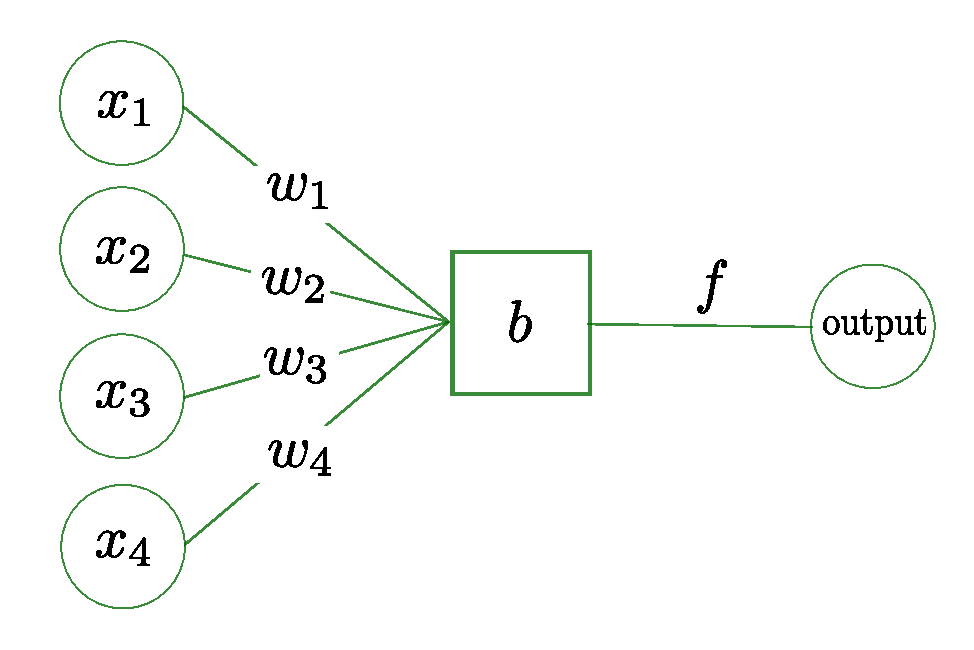
\includegraphics[width=0.6\columnwidth]{C4_cnn/neuron.pdf}
    \caption{Basic neuron}
    \label{machine:nn:neuron:plot}
\end{figure}

In the example in Fig.~\ref{machine:nn:neuron:plot} I have shows a neuron which has 4 input variables, or 4 input data points. 
When a network is trained, or when it learns, the weights applied to each of the inputs and the bias are updated to better represent the input data.
This training procedure is explained in more detail in Sec.~\ref{machine:nn:training}
Many neurons are then used in combination with each other to develop a neural network which can be applied to more complex problems.

%%%%%%%%%%%%%%%%%%%%
\subsection{\label{machine:nn:structure}Network structure}
%%%%%%%%%%%%%%%%%%%%

The structure of a neural network is defined by the user and there is no set way to design a network.
However, the general layout of a neural network is defined by structures called layers, sometimes known as fully connected layers. 
These are rows of $N$ neurons which all take the same input such that there is $N$ output values.
An example of a simple neural network is shown in Fig.~\ref{machine:nn:structure:plot}.
The first layer is the input layer, this is just the data points from an input example.
In the example of hand drawn digits, this would be the pixels from the image of the digit.
The final layer represents the information that you intend the network to extract from the input data. 
In the hand drawn digit example, this could have 10 output values corresponding to each digit 0-9. 
Each of these outputs is then a value which is related to the probability of that digit being present in the image.  

When designing a network, the user will have a defined input layer size from the data and a set number for the output layer which represents, for a classification example, the number of output classes. 
The number of hidden layers and the number of neurons in those hidden layers can be arbitrarily changed. 
In general if the data contains more complex information the size or complexity of the network will need to be increased for it to be able to extract the information. 
If there is a small number of training examples and a large and complex network, it may be able to learn the input data set as opposed the the general information that they represent.

\begin{figure}[h]
    \centering
    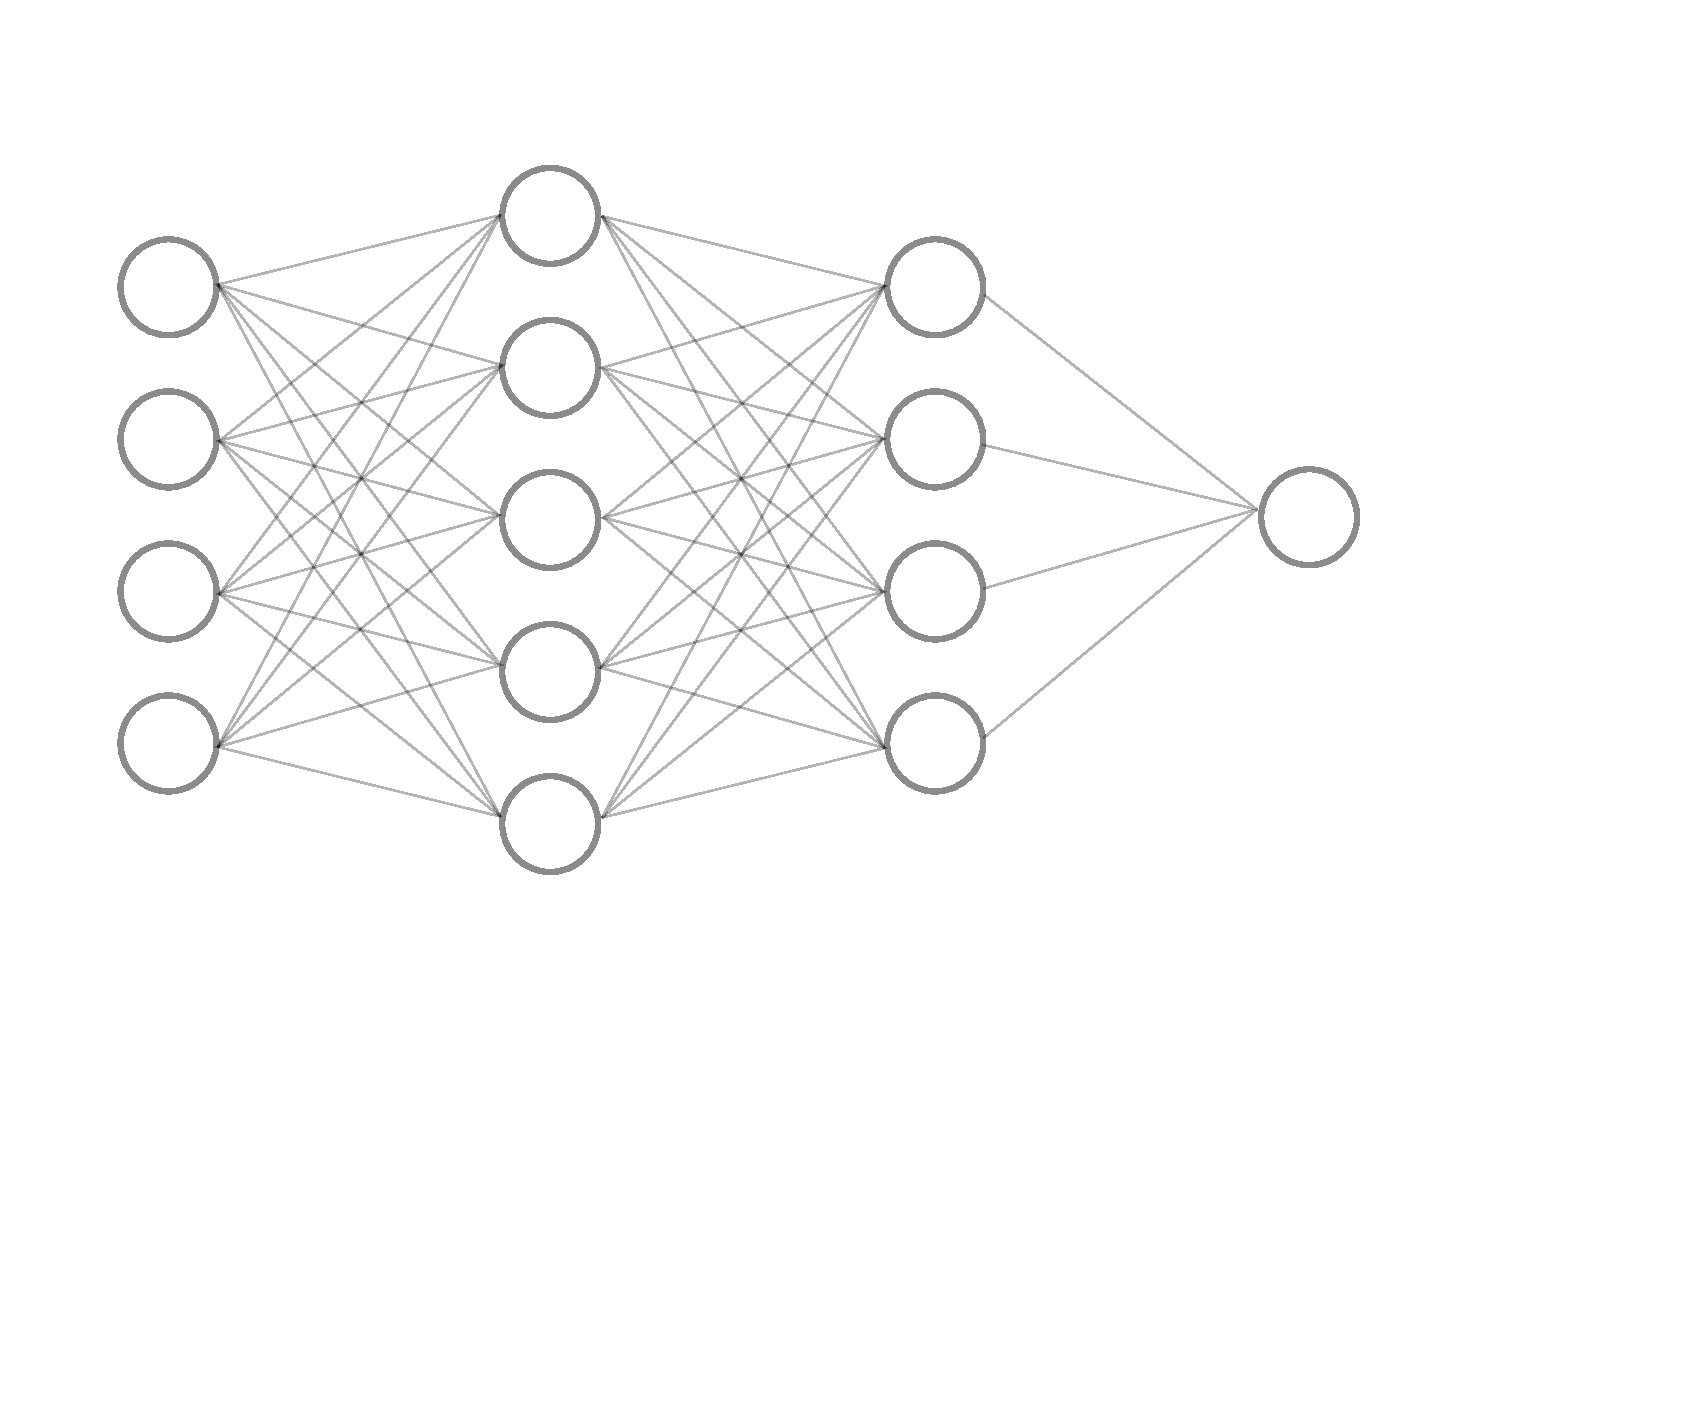
\includegraphics[width=\columnwidth]{C4_cnn/simple_network.pdf}
    \caption{A neural network is structured with layers. Each of the circles in these layers are neurons as described in Sec.~\ref{machine:nn:neuron} and Fig.~\ref{machine:nn:neuron:plot}. The networks contain an input layer which is usually the data which you would like to analyse. Then this passes to a number of `hidden' layers, in the above diagram there are two. Hidden layers are just layers which exist between the input and the output. The output layer is then the desired output, above I have chosen a single neuron as output. This is such that the network could classify the input to a value between 0 and 1. Every neuron in a layer is connected to the output of all neurons in the previous layer.}
    \label{machine:nn:structure:plot}
\end{figure}


%%%%%%%%%%%%%%%%%
\subsection{\label{machine:nn:activation}Activation functions}
%%%%%%%%%%%%%%%%%

The activation function is how the output of a neuron is transformed. 
The most simple activation function is a cut as described in Sec.~\ref{machine:nn:neuron}, however, this type of activation does not perform well.
Activations functions a generally based on a few properties.
The activation function is generally non-linear, this allows networks with multiple layers to be used to approximate a function. A linear activation function means that any number of layers in a network is equivalent to a single layer network.
Another property which is desired in activation function is that it is continuously differentiable. This is to allow algorithms such as gradient descent to optimise the network. 
The functions are found to perform better if they are monotonic and smooth.
There are many choices when defining this in the network, some of the available options are shown in Fig.~\ref{machine:nn:activation:plot}.
One of the more commonly used activation function is the LeakyRELU function, this is explained in more detail in \citep{maas2013RectifierNonlinearities}.
In the work that follows we use the Leaky RELU function and the sigmoid function.


\begin{figure}[h]
	\centering
	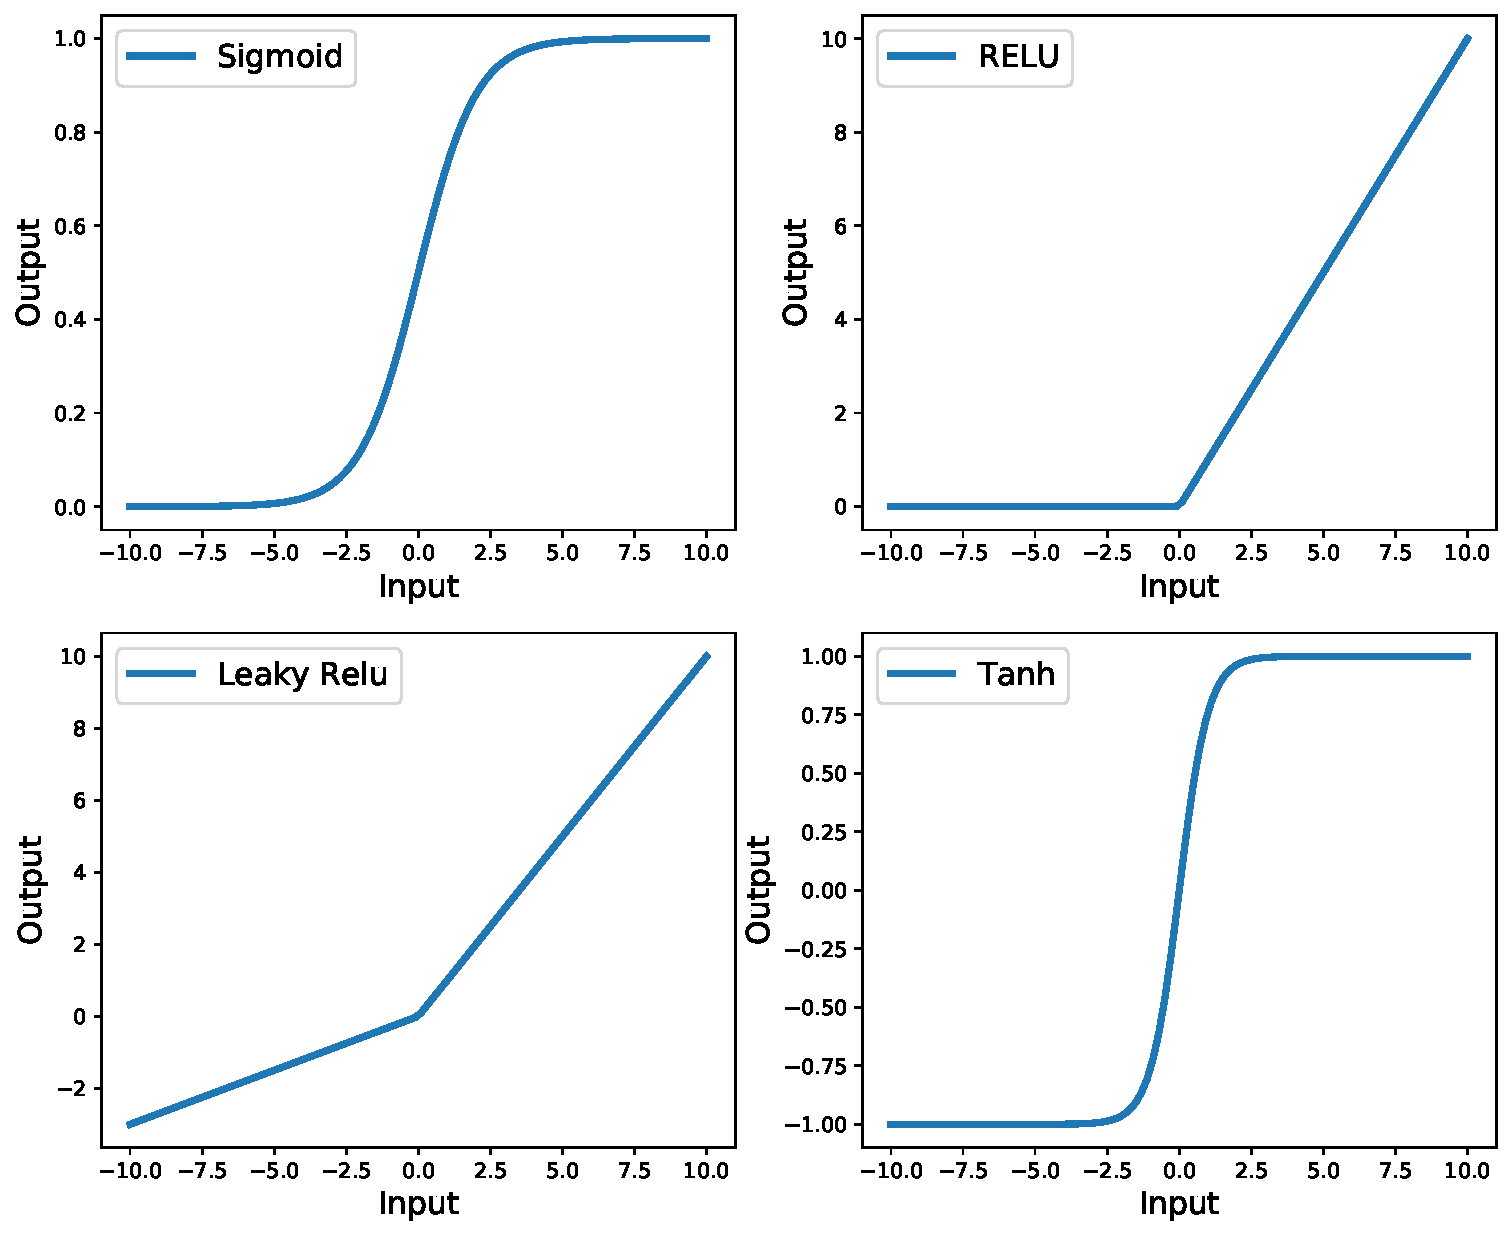
\includegraphics[width=0.8\columnwidth]{C4_cnn/activations.pdf}
	\caption{There are many different activations function which are used, and essentially any function can be defined if necessary. Above is shown a subset of the more commonly used functions. The linear function is not used, however, is there to compare to common non linear function.}
	\label{machine:nn:activation:plot}
\end{figure}





%%%%%%%%%%%
%%%%%%%%%%%
\section{\label{machine:cnn}Convolutional Neural Networks}
%%%%%%%%%%%
%%%%%%%%%%%

\acp{CNN} are a different type of deep neural network than in Sec.~\ref{machine:nn}.
They are a types of network which are primarily used in image
processing and recognition
\cite{lecun2015DeepLearning,lecun1998GradientbasedLearning,waibel1989PhonemeRecognition,krizhevsky2012ImageNetClassificationa}.
Here the general idea is summarised. 
A \ac{CNN} is designed to take in data, identify different features within that data and classify
what those features or combinations of those features mean.
In the context of this work the input data is a time-frequency spectrogram which may contain a simulated \ac{CW} signal.
The output is then a single number which represents if a signal is present.
Here a value of 1 represents a signal and 0 is not a signal.
A \ac{CNN} can learn how to identify features by being trained on many
examples of the input data where the output is known.
For example, an input spectrogram with a simulated \ac{CW} signal would have an output value of 1.
Given the set of training examples, the many parameters of the \ac{CNN} can
be updated such that it gives the best result for any new image. 
This process is the same as neural networks in Sec.~\ref{machine:nn} and will be described in greater detain in Sec.~\ref{machine:training}

The key features of \acp{CNN} which distinguish them from ordinary neural networks is some additional types of layers including: Convolutional layers and max pooling layers. 


%%%%%%%%%%
%%%%%%%%%%
\subsection{Convolutional layers}
%%%%%%%%%%
%%%%%%%%%%

Convolutional layers have some similarities to standard fully connected layers as described in Sec.~\ref{machine:nn:structure}. 
The main difference being how the weights are applied to the inputs.
A fully connected neural network would flatten this image and apply Eq.~\ref{machine:nn:neuron:equation} to the inputs.
This involves having a separate weight for each of the input pixels in an image.
A convolutional layer however, filters the image and outputs a filtered image of the same size (the image can be a different size it depends how the layer was set up).
This convolution is defined by,
\begin{equation}
\label{machine:cnn:conv:equation}
O_{i,j} = f\left( \sum_{m} \sum_{n} F_{m,n}x_{i-m,j-n}\right) ,
\end{equation}
where $O$ is the output image, $x$ is the input image, $F$ is the convolutional filter and $f$ is the activation function.
The weights of the filter $F_{m,n}$ are what are updated when the network is trained.
Fig.~\ref{machine:cnn:convlayer:input} shows an example of a 6x6 image and the results of filtering the image using Eq.~\ref{machine:cnn:conv:equation} with two different filters $F$. 
In this case the network has 4 parameters for each filtered image which can be updated as opposed to the 36 which a full connected network would have for a single neuron.

Fig.~\ref{machine:cnn:convlayer:input} demonstrates how a filter which matches a feature in an image can highlight that particular feature. 
i.e. the diagonal line in the bottom left of the input is enhances by Filter 1, which matches that feature. 
When this type of layer is trained, the weights of the filter are updated. The filter should then ideally match the feature which is intended to be extracted.

\begin{figure}[p]

    \centering
    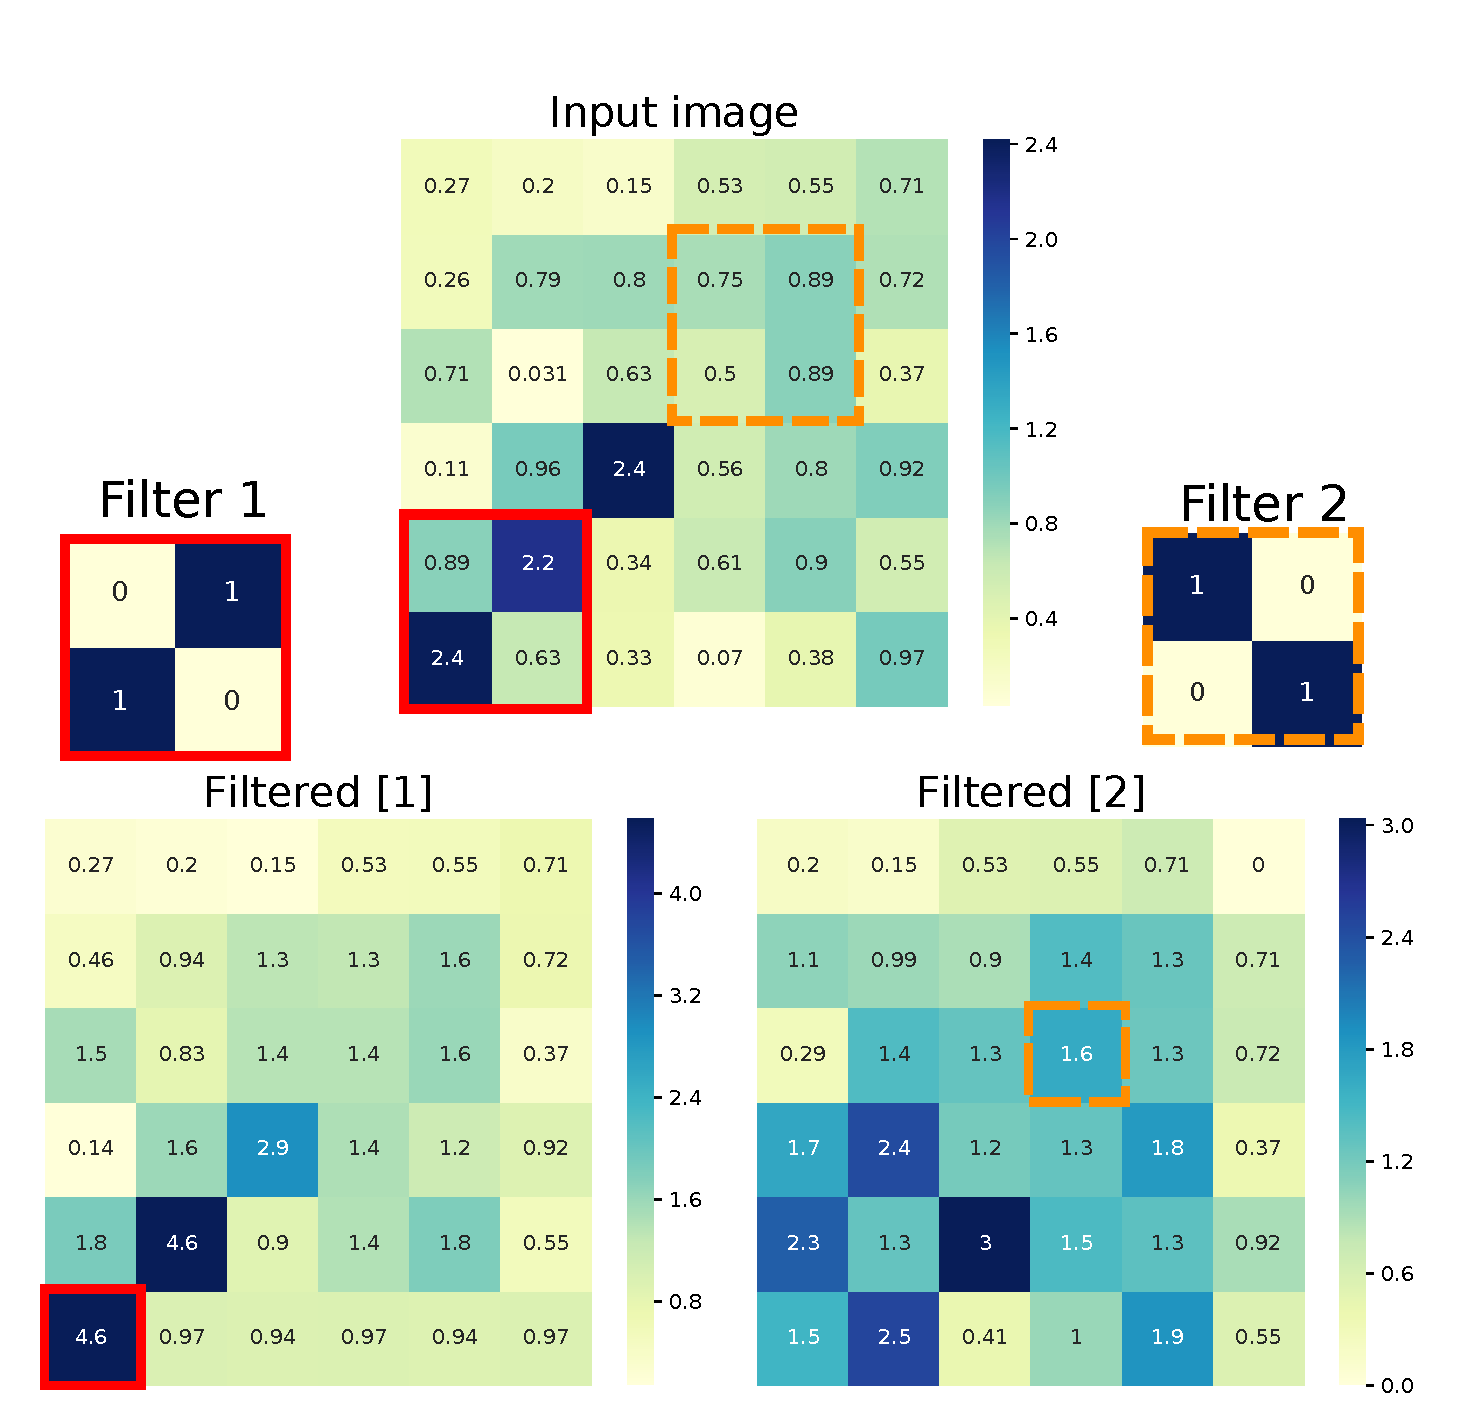
\includegraphics[width=\columnwidth]{C4_cnn/conv_filters.pdf}
    \caption{Convolutional filters can be designed to `pick out' certain features within an image. In this simple example above, the first filter (filter 1) matches the diagonal line in the bottom left of the input better than filter 2. The output filtered image the exaggerates this filter. The coefficients of the filter i.e. $F_{m,n}$ in Eq.~\ref{machine:cnn:conv:equation}, in this are set to ones and zeros.
    These are the weights which are trained by the network. In this an cases that follow, to get the same size image in the output as the input, the image is padded with zeros. I this image it was necessary to pad above and to the right of the image. The output of a convolutional layer is then the filtered images above after a bias and activation function have been applied. }
    \label{machine:cnn:convlayer:input}

\end{figure}

A convolutional layer has a number of different hyper-parameters which can be varied when setting up a model.
Below I list each of the adaptable parameters and what they do.

\begin{description}
\item[Filter size] The filter size is the size and shape of the convolutional filter. In Fig.~\ref{machine:cnn:convlayer:input} we use a filter size of 2$\times$2. The filter does not have to be square, however must be less than the dimensions of the image.

\item[Number of filters] The number of filters can be any value. If you have $K$ filter kernels, then the convolutional layer will output $K$ filtered images. In Fig.~\ref{machine:cnn:convlayer:input} we use two filters and therefore, the output of the layer is two images.

\item[Activation function] The activation function is generally kept the same for each of the layers, however this can be set here. The different types have been explained in Sec.~\ref{machine:nn:activation} and are applied as in Eq.~\ref{machine:cnn:conv:equation}.

\item[Stride] A normal convolutional layer applies a filter by multiplying by a filter, then shifting over by one pixel and repeating. Applying a stride mean rather than shifting by one pixel, one shifts by a number greater than one. This reduces the size of the output by the same factor of stride. i.e. if you skip one pixel (a stride of 2) then the image will be half the size on output. This has a similar affect to max-pooling which we describe in Sec.~\ref{machine:cnn:maxpool} an use for the rest of this work.  
\end{description}

The convolutional layers with reduce the number of updatable parameters used in each network or model.
However, the output of a convolutional layer is a number of images which ar potential the same size as the input. 
This has potentially increased the size of the parameter space for the next layer.
To decrease this a type of layer known as max-pooling is used.

%%%%%%%%%
%%%%%%%%
\subsection{\label{machine:cnn:maxpool}Max pooling layers}
%%%%%%%%%%%%
%%%%%%%%%%%

Max pooling layers are designed to reduce the size of the problem whilst holding on to as much important information as possible.
These do not contain any trainable parameters.
The idea of this layer is relatively simple, it reduces the image size by taking the maximum value in a region of a given size.
Fig.~\ref{machine:cnn:maxpool:image} shows the output of the first filtered image in Fig.~\ref{machine:cnn:convlayer:input}.
The image is then reduced by a 2$\times$2 max pooling layer.
The output of max-pooling Then shows a large value in the bottom left, this is where the input image matched the filter in Fig.~\ref{machine:cnn:convlayer:input}.
This demonstrates how the max-pooling layer can hold on to important information whilst reducing the image size.

\begin{figure}[h]
    \centering
    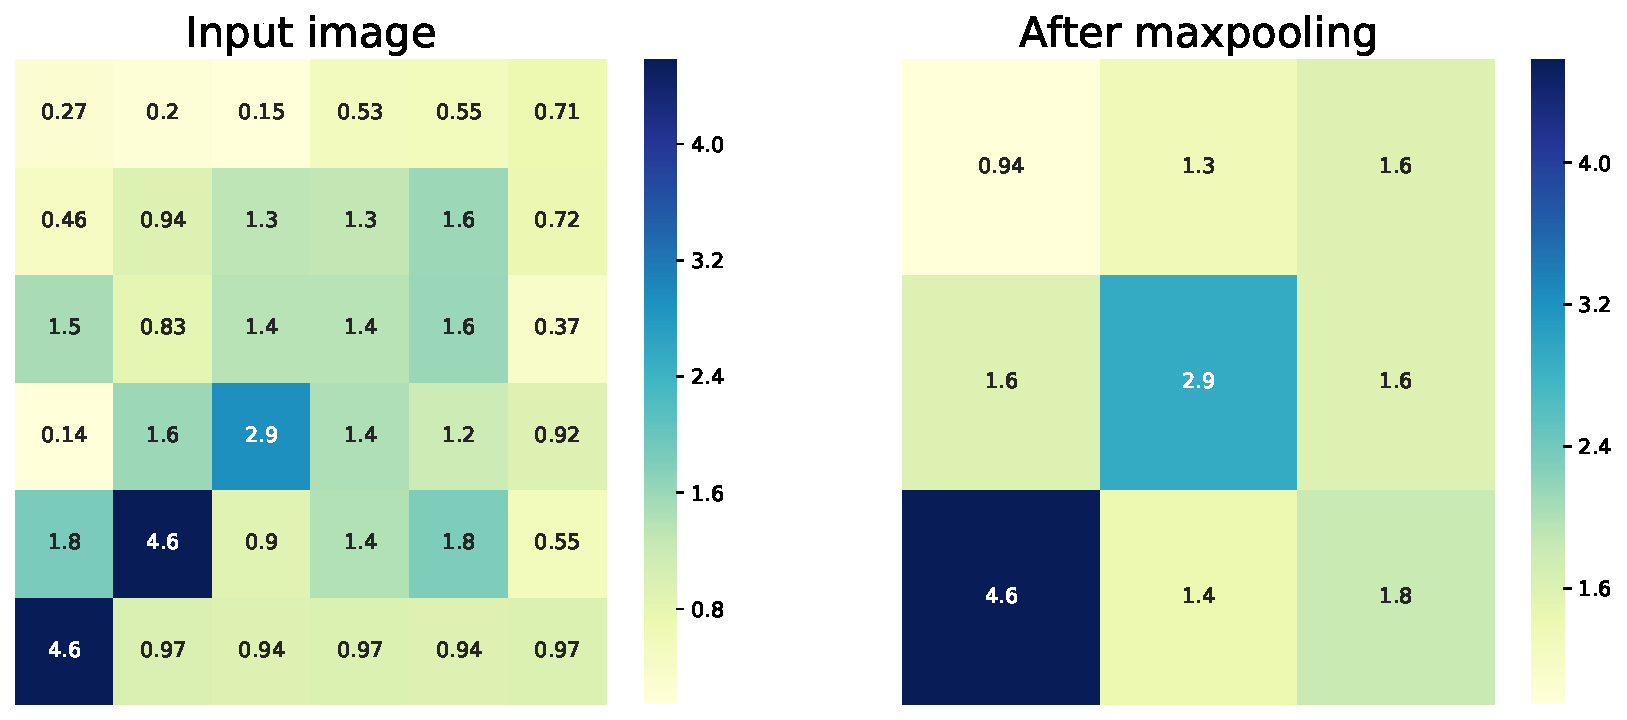
\includegraphics[width=\columnwidth]{C4_cnn/maxpool.pdf}
    \caption{Max pooling layers aim to reduce the size of am image whilst retaining important information within the original image. Above shows an example where a 2$\times$2 max-pooling layer is used on the output of Filter 1 in Fig.~\ref{machine:cnn:convlayer:input}. This retains the information that the input image matches the filter in the bottom left.}n
    \label{machine:cnn:maxpool:image}
\end{figure}

%%%%%%%%%%%%%
%%%%%%%%%%%%%%
\subsection{CNN structure}
%%%%%%%%%%%%%%
%%%%%%%%%%%%%%

\acp{CNN} are usually structured such that they can extract larger features from an input image, then the outputs from this are passed on to be classified.
The `feature extraction' part of the network consists of the convolutional layers and the max-pooling described in Sec.~\ref{machine:cnn}.
The outputs of the final max-pooling layer are then flattened and used as the input to a fully connected network.
This fully connected network the classifies these outputs into a number of classes.
Fig.~\ref{machine:cnn:structure:example} shows an example of the layout. 
Here an input image which is the same as in previous examples is passed onto a single convolutional layer with two different filters.
The output of two filtered images is passed to a max-pooling layer.
The two max-pooled images are flattened into 18 input neurons, this then passes through a fully connected network to a single output neuron.
This shows a simple example, however, there are many hyper-parameters of the network which can be changed.
These include: the number of filters in a convolutional layer, the number of convolutional layers and max-pooling layers, the number of hidden layers in the fully connected section and the number of neurons in the hidden layers. 
This example also shows the network being classified to a single output as this is how we use \acp{CNN} for the following work.

\begin{figure}[h]
	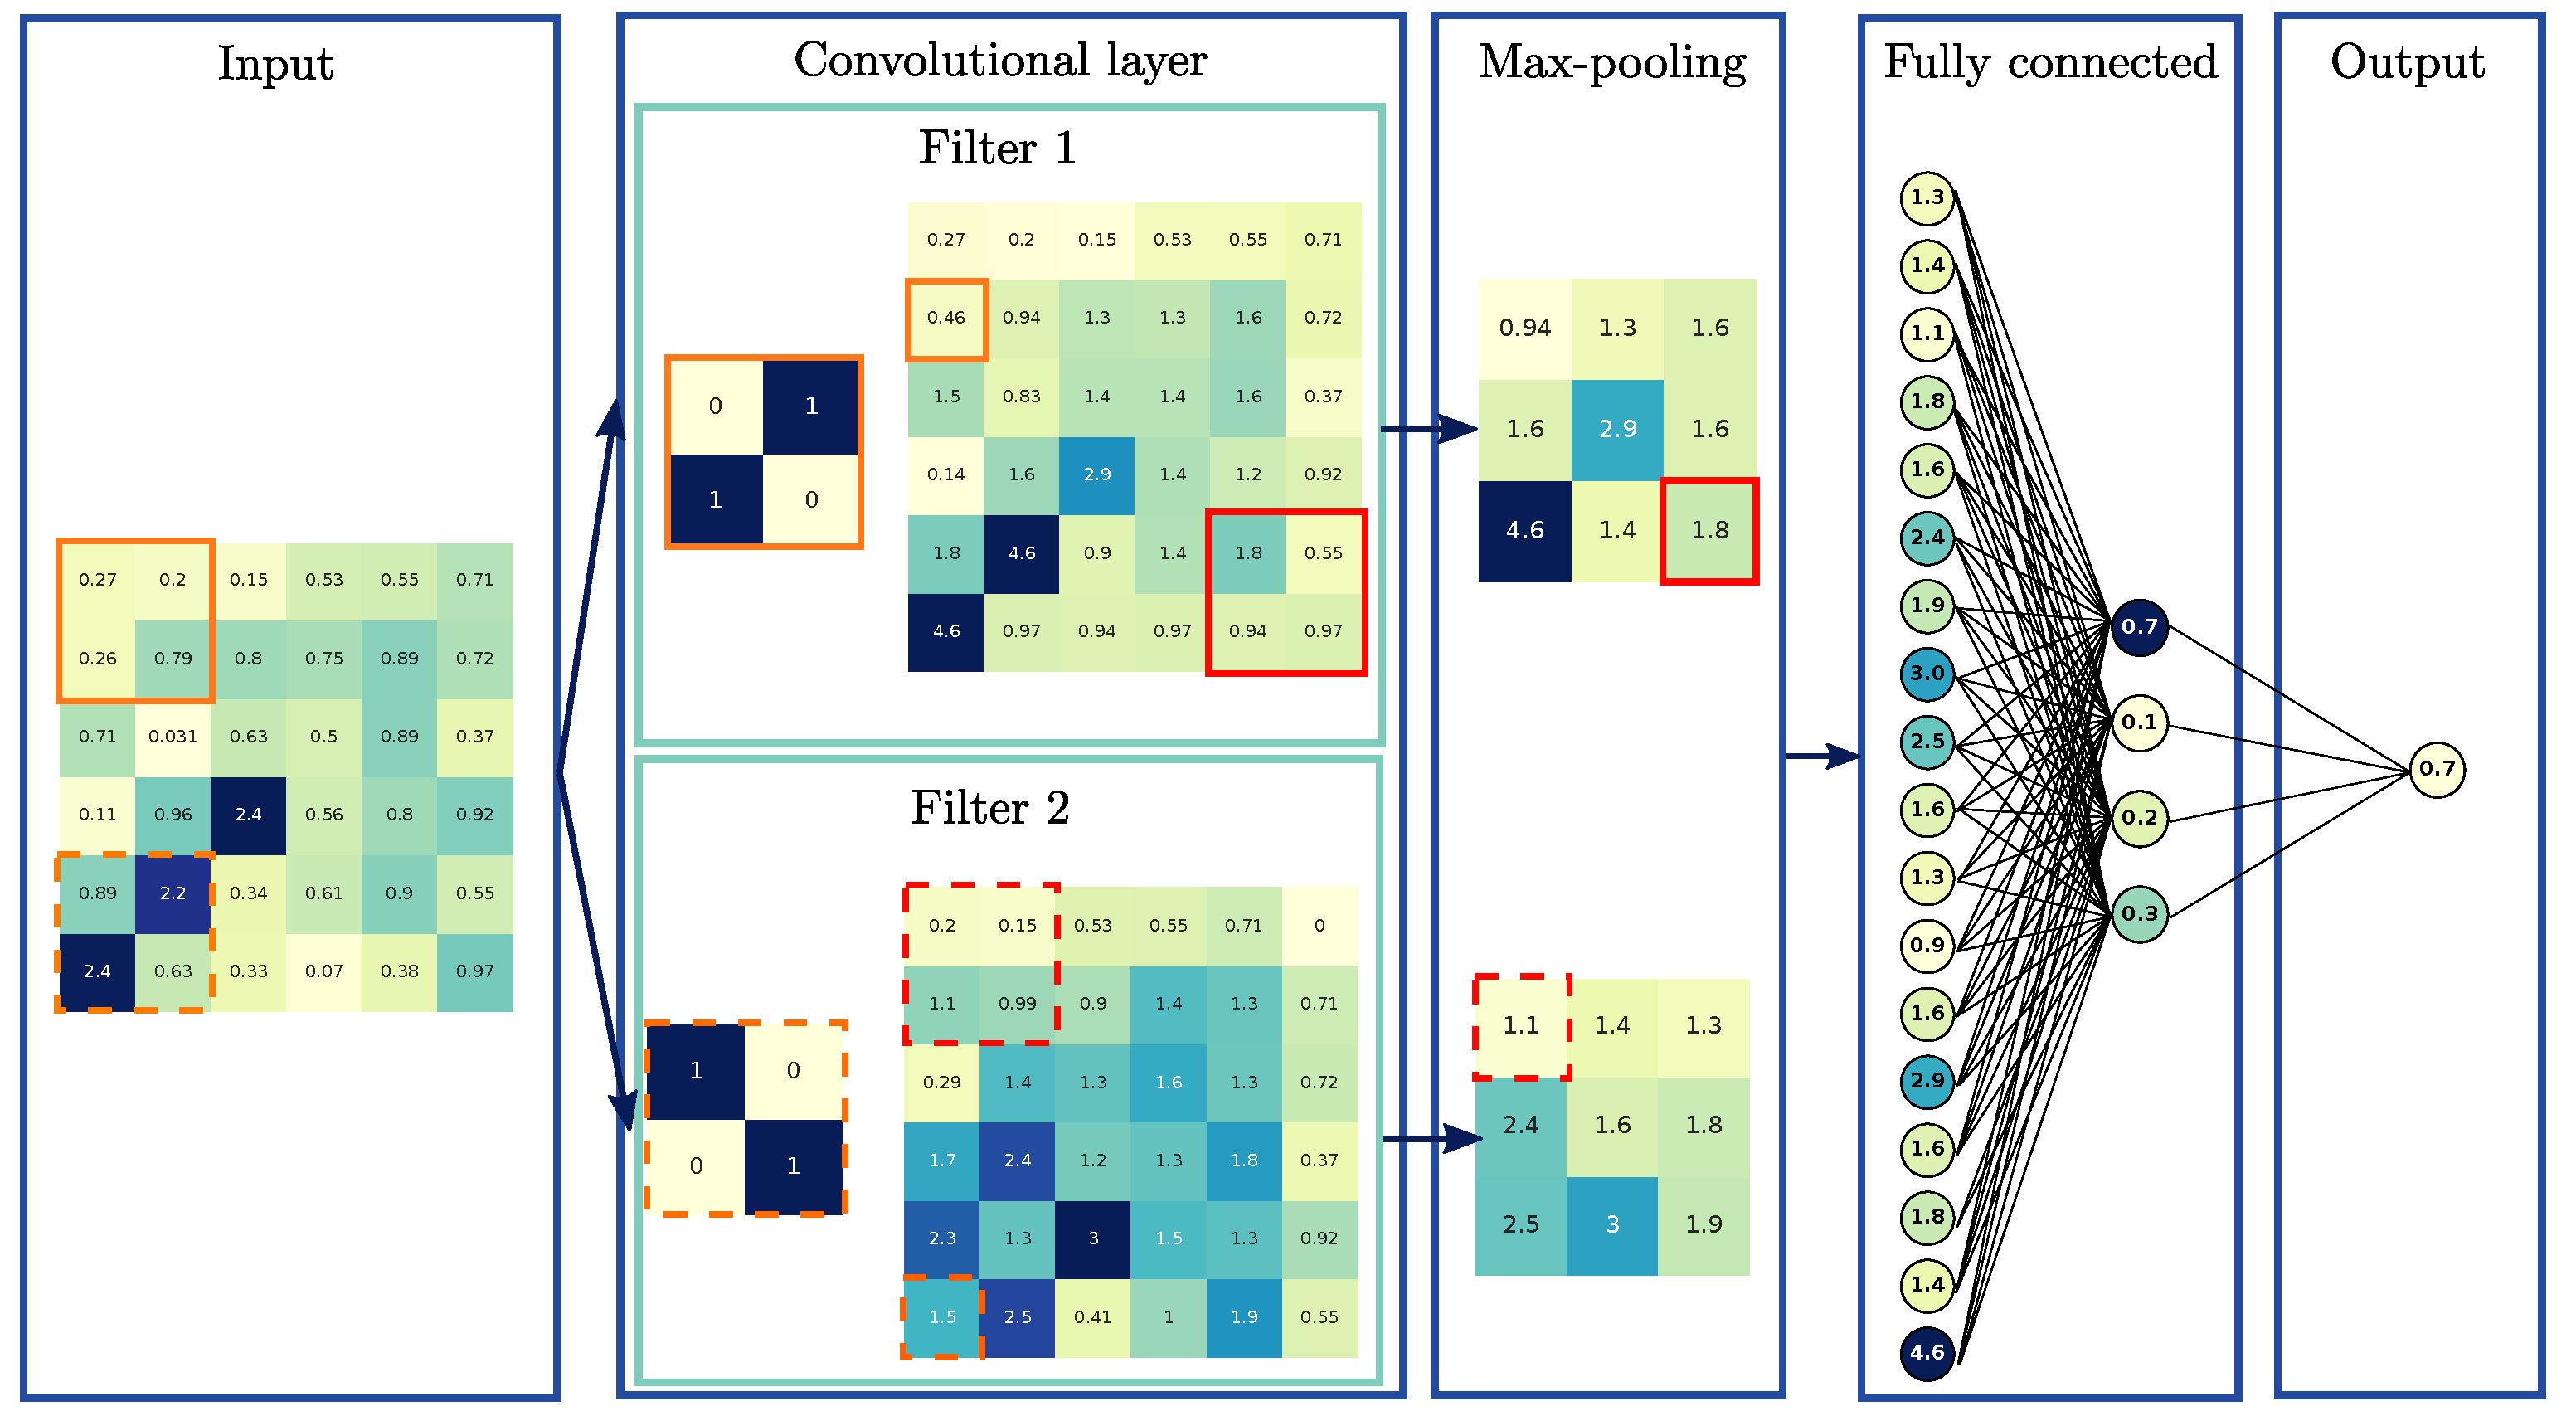
\includegraphics[width=\textwidth]{C4_cnn/cnn_structure_ex.pdf}
	\caption{Convolutional neural networks consist of two broad sections, the `feature extraction' part which is the convolutional and max-pooling layers, and the classification part which is the fully connected part of the network. This diagram shows a simple example of an image passing through a single convolutional layer with two filters, a single max-pooling layer and a simple fully connected network with a single hidden layer consisting of 4 neurons. }
	\label{machine:cnn:structure:example}
\end{figure}


%%%%%%%%%%%%%%%%%
\section{\label{machine:training}Training}
%%%%%%%%%%%%%%%%%

% introduce training concept
%
Once the structure of the network is decided, the network needs to be trained.
This means that the weights and bias' for every neuron and filter need to be updated such
that the neural network gives a useful output. For this
work we will classify the input images using a single output neuron.
This neuron outputs a value between 0 and 1 using a sigmoid function.
The \ac{CNN} is trained using a process called supervised
learning. When using supervised learning, the class of each input example is know. For example, we assign a label of 1 when the
input is a time-frequency spectrogram which includes a simulated \ac{CW}
signal. Similarly a time-frequency spectrogram with no simulated signal is assigned a label of 0. 
In general when training neural networks this way, the performance of the network can be improved by increasing the number of input examples which are shown to the network.
This stops the network from over-fitting to specific examples. Instead it should generalise to the full input and learn the underlying features within the data.

\subsection{Loss function}

%Training procedure
%
Each of the training examples is then propagated though the network to its single output value which lies between 0 and 1. Using a loss function, this output is then be compared to
the label of the input data which is either 0 or 1. There are many types of loss function which can be used, this depends on the type of problem which one wants to solve. As we are classifying
between two classes in out networks, the loss function, $L$, is the binary
crossentropy defined as,
%
\begin{equation}\label{cnn:loss} 
L = -y\log{(p)} + (1-y)\log{(1-p)},
\end{equation}
%
where $p$ is the networks predicted output which has any value in the range $[0,1]$ and $y$ is the true output which has binary labels 0 or 1. 
The loss function is minimised when the output matches the truth. This essentially
tells the neural network how close to the truth it is. The weights and bias' of
the neural network can be updated based on the value of this loss function. The
process of updating the weights and other parameters is called back-propagation,
and typically uses a form of gradient descent
\cite{kingma2015AdamMethod}.
Back-propagation uses the derivative of the loss function with respect to a weight to update that weight.
If changing that weight in a particular direction decreases the loss function, then the weight will be updated in that direction.
The size of the change of the weight value is related to the change in the size loss function.
This means that the weights can be updated to minimise the loss function and therefore improve the performance of the network.

%%%
%%%
\subsection{Training procedure}
%%%
%%%

The training procedure entails passing a set of training examples through the network a number of times. 
Once the entire training data set has been passed through the network (forward pass) and the weights have been updated accordingly (back propagation), the training has completed one epoch.
If the data was passed and the weights were updated a single time, the loss may decrease by is likely not at a minimum.
Passing the data through again may move the weights to a lower loss.
This process is repeated a number of times to try and find the minimum loss.

If for example the network is large, i.e. it has many trainable parameters, and the data set contains simple features, then the network can over train.
This mean the network learns specific features of the data-set rather than a general representation of it. 
To monitor this, after each epoch of training the loss is measured on a subset (test set) of the data which was not used for training. 
If the loss of the training set decreases but the loss of this test set begins to increase, then this is an indicator of over training. 

\joe{need to say somewhere what this actually does, i.e. why its useful}





%%%%%%%%%%%%%%%%%%%%%%%%%%%%%%%%%%%%%%%%%%%%%%
%%%%%%%%%%%%%%%%%%%%%%%%%%%%%%%%%%%%%%%%%%%%%%%%
\section{\label{machine:cw}Application to CW search}
%%%%%%%%%%%%%%%%%%%%%%%%%%%%%%%%%%%%%%%%%%%%%%%%%
%%%%%%%%%%%%%%%%%%%%%%%%%%%%%%%%%%%%%%%%%%%%%%%

The aim for this work is to use a \ac{CNN} to classify \ac{LIGO} data into one of two classes: signal or noise.
Here the signal class refers to a \ac{CW} signal from an isolated neutron star as described in Sec.~\ref{searchcw:model}.
Noise then refers to anything else which appear in the data, from Gaussian noise to instrumental artefacts. 
In Sec.~\ref{soap:results} to reduce the effect of instrumental artefacts, each of the search sub-bands was analysed by eye to determine if a sub-band was contaminated. 
Sub-bands which contained an artefact were then removed from the search.
This is a time consuming process. The main goal of the \ac{CNN} approach is to automate this part of the search.
This section will describe how we design the network to extract features and distinguish signals from instrumental artefacts.
We will then present results form searches in a range of \ac{LIGO} observing runs which include: S6, O1 and O2.


%%%%%%%%%%%%%%%
%%%%%%%%%%%%5%%
\subsection{\label{machine:cw:structure}Network structure}
%%%%%%%%%%%%%%%
%%%%%%%%%%%%%%%

In this section the structure of the networks which are used in this analysis
are described. There are three main inputs of data for each \ac{CNN}: spectrograms, Viterbi maps and the Viterbi statistic. Each of these are different representations of the raw detector data. In this analysis we train a separate \ac{CNN} for each of
these inputs and then a further three which use these combinations of inputs:
Viterbi map + spectrogram, Viterbi map + Viterbi statistic and Viterbi map +
Viterbi statistic + spectrogram. In all of the layers excluding the output layer of each \ac{CNN}, the activation functions in Eq.~\ref{machine:cnn:conv:equation} and \ref{machine:nn:neuron:equation} are defined by a function titled `leakyRELU' \cite{maas2013RectifierNonlinearities}. 
For our output neuron a sigmoid function is
used as an activation function such that the output is limited between 0 or 1.
For a given input a \ac{CNN} can then output a value between 0 and 1. When the output value is closer to 1, the input is more likely to contain a signal. 
The output value can then be treated as a detection statistic. 
The structure of the network is shown in Fig.~\ref{machine:results:cnnlayout} and is explained below. 

\begin{description}
	\item [Viterbi statistic] This is the simplest of the networks and will
	give the exact same result as the Viterbi statistic on its own. This is a
	single neuron which takes in the Viterbi statistic applies a weight and bias
	and then passes through a sigmoid function.
	
	\item [Viterbi map] The Viterbi map \ac{CNN} takes in a down-sampled Viterbi map of size (156,89), this is described more in Sec.~\ref{machine:data:downsample}.
	This \ac{CNN} consists of two convolutional layers and 3 fully connected layers. The first layer has
	8 filters which have a size of $5\times5$ pixels, the second layer has 8
	filters with a size of $3\times3$ pixels. After each of these layers we use a
	max-pooling layer with a size of $8\times8$ pixels. This then passed into three
	fully connected layers which all have 8 neurons and used leakyRELU activation
	functions. Finally these lead to an output neuron which uses a sigmoid
	function.
	
	\item [Spectrogram] The spectrogram \ac{CNN} takes in a down-sampled spectrograms of size (156,89), this is described more in Sec.~\ref{machine:data:downsample}.
	This \ac{CNN} has an identical structure as the Viterbi map \ac{CNN}, however, takes two channels as input. The two channels are the spectrograms of two different detectors.
	
\end{description}

The next three networks are constructed from combinations of the previous described \acp{CNN}.

\begin{description}
	\item [Viterbi map and spectrogram] To combine the spectrogram and Viterbi map network, we remove the final output neuron and its 8 weights from each of the networks. 
	The outputs from each network is then 8 neurons. These can be combined to a single sigmoid neuron which has 16 new weights.
	
	\item [Viterbi map and Viterbi statistic] In this network we combine the
	Viterbi statistic with the Viterbi map. As before, this uses the pre-trained
	Viterbi map and Viterbi statistic \acp{CNN}. The output sigmoid neuron and corresponding weights are removed from each network. 
	The 8 neurons from the Viterbi map network and the single neuron from the Viterbi statistic network are then combined to a single neuron with 9 new weights.
	
	\item [Viterbi map, Viterbi statistic and spectrogram] This combination takes all component \acp{CNN} from above. As before the final sigmoid output and the corresponding weights from each network are removed.
	The 8 neurons from the Viterbi map and spectrograms \acp{CNN} and the single neuron from the Viterbi statistic are then joined into a single output neuron with 17 new weights. 
	
\end{description}

When combining \acp{CNN} we use a process called transfer
learning~\cite{prattDiscriminabilityBasedTransfer}. This uses the pre-trained weights of the networks as a starting point to continue training. 
In our examples we found that we could fix the weights inside the pre-trained networks and just train the final 16 output weights from the neurons as in Fig.~\ref{machine:results:cnnlayout}.
These combinations of networks were chosen as the different representations of the data should contain slightly different information on the input.
For example, the Viterbi statistic contains no information on the structure of the track in the data and the Viterbi maps lost some information about lines in the band.
The addition of the spectrograms aimed to include even more information about this piece of data. 
Where when each of these are combined, the \ac{CNN} should be able to pick to important information from each of these representations.

% plot of vitmap and spretrogram structure 
%
\begin{figure}[p]
	\centering
	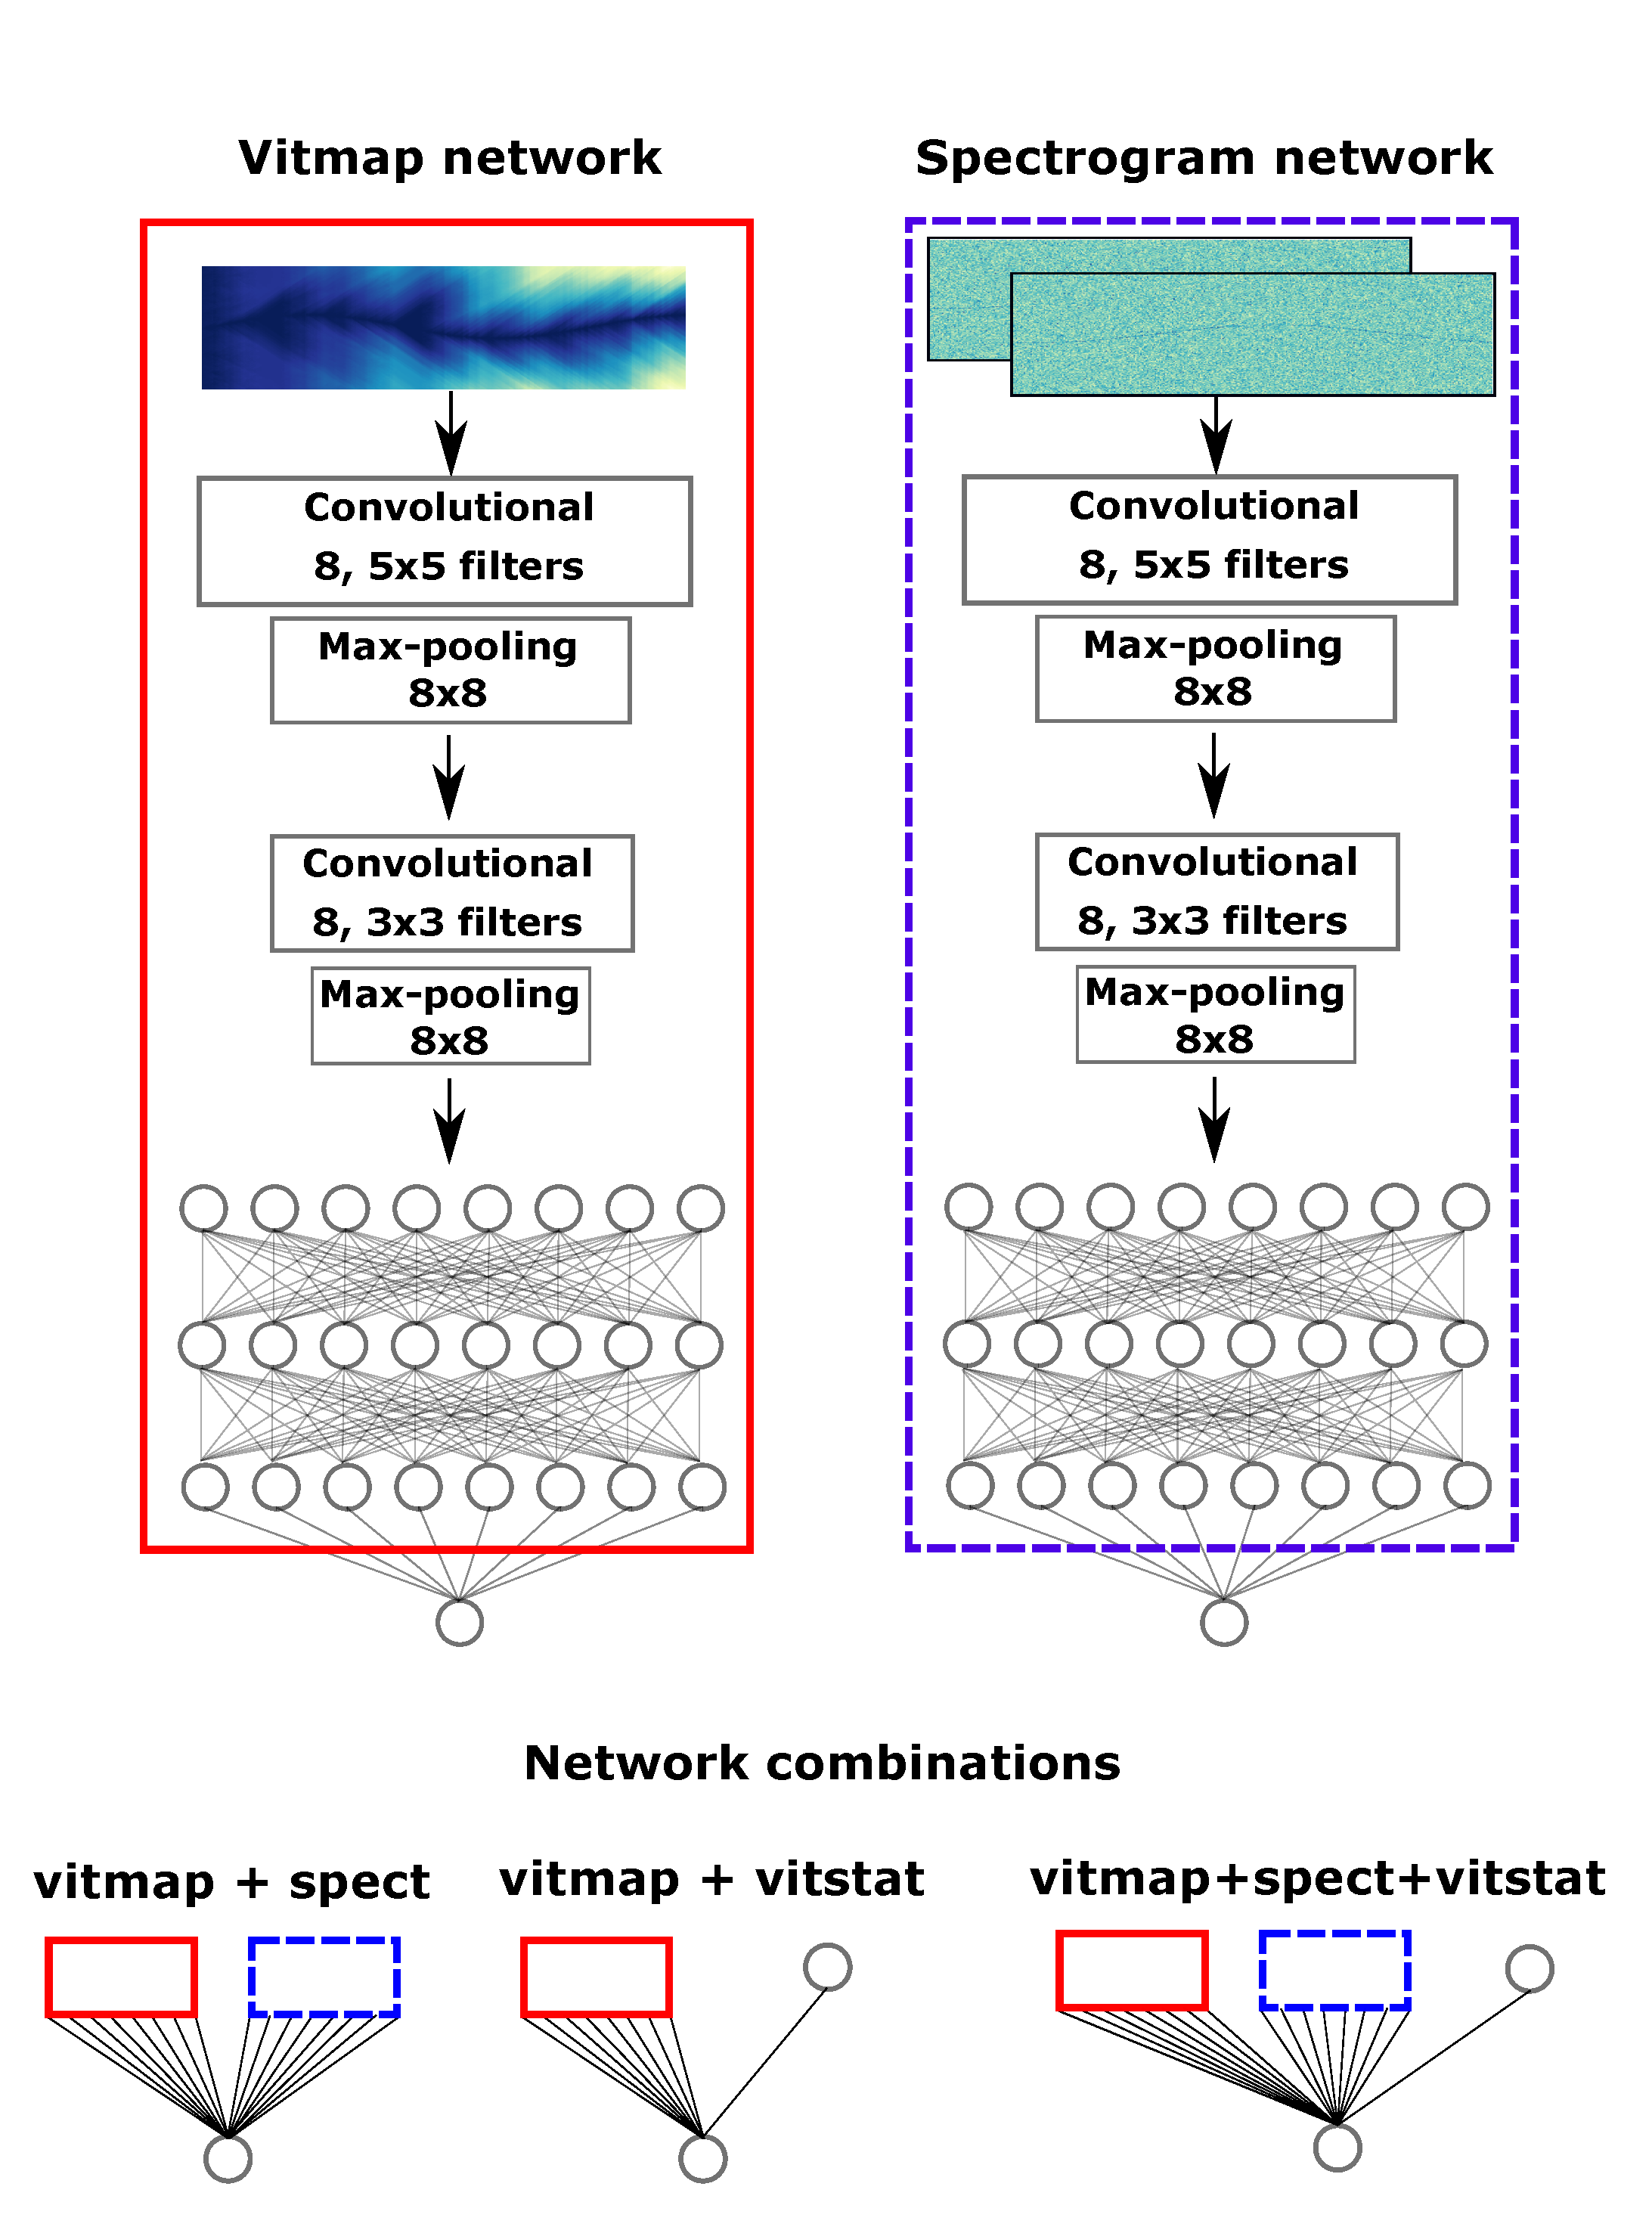
\includegraphics[width=0.9\columnwidth]{C4_cnn/networks.pdf}
	%
	\caption{\label{machine:results:cnnlayout} The structure of the Viterbi map and
		spectrogram \acp{CNN} used in this analysis are the same, with the difference
		that the spectrogram takes two images as input. They each use two convolutional
		layers and 3 fully connected layers before they're output to a single neuron which represents the probability of belonging to the signal class. The
		Viterbi statistic network is a single neuron that transforms the statistic into
		a number between 0 and 1 representing the probability of belonging to
		the signal class. For the combinations of networks, we remove the final
		output neuron and its 8 weights, i.e. we take the part inside the red or blue box. The 8 outputs from each network are then combined to a single neuron with 16 new weights. }
	%
\end{figure}


%%%%%%%%%%%%%%%%%%%%%%%%%%%%%%%%%%%%%%
%%%%%%%%%%%%%%%%%%%%%%%%%%%%%%%%%%%%%%
\section{\label{machine:data} Data generation}
%%%%%%%%%%%%%%%%%%%%%%%%%%%%%%%%%%%%%%
%%%%%%%%%%%%%%%%%%%%%%%%%%%%%%%%%%%%%%

% define the 3 data types that we consider
%

For the analysis that follows there are three main sets of data: training data,
testing data and search data. 
Training data is a set of data containing simulated signals which is used to train each of
the networks.
Test data is a separate set of simulations which is used to generate
efficiency curves and test the network.
Search data does not contain any simulated signal injections and is used to search for real signals.
For the majority of the analysis that follows, we use real detector data for all three of these data-sets, the exact observing runs will be explained in Sec.~\ref{machine:results}. 
The noise in real data contains many non Gaussian features, a particular class of these is known as instrumental lines and they have a large affect on \ac{CW} searches. 
The aim is to have a network which does not 
\joe{still trying to think how to write}
Each of these use
real data as it becomes difficult to simulate the many different classes of
instrumental line. The real data contains all the types of instrumental lines
which we need the network to identify.~\chris{this paragraph is a bit fluffy.
	Maybe say upfront that all data used is real detector data but then actually
	specify which real detector data O1,O2 etc... and give references. Also add a
	bit more about the detector lines. Maybe add that for each type of data you
	generate all 3 types of data product as defined in the previous section.} 

% describe the idea of odd and even bands
%
When training and testing a network it is important that the networks are not
trained and tested on the same data. Otherwise the \acp{CNN} can learn specific
features of the training data and not the underlying
distribution of features. To avoid this, the spectrograms are split into $0.1$
Hz wide sub-bands where alternating bands are designated as `odd' or `even'.
This means that bands starting with 100.1,100.3 are odd and 100.2,100.4 are
even etc. The networks can then be trained on the odd bands and tested on the
even bands and vice versa.
This then means that each time we want to search over data, we will have two final networks. One which will be run on odd bands and a separately trained network which is run on even bands. 

%%%%%%%%%%%%%%%%%%%%%%%%%%%%%%%%%%%%%%%%%%%%%%%%%%%%%%%
\subsection{\label{machine:data:injections} Signal simulations}
%%%%%%%%%%%%%%%%%%%%%%%%%%%%%%%%%%%%%%%%%%%%%%%%%%%%%%%

% describe signal injection
%
To inject the simulated signals into real data we generate a random set of signal
parameters which are drawn from prior distributions defined in
Table~\ref{machine:data:injections:table}. The \ac{SNR} of each simulation is then uniformly distributed between 50 and 150. Where the \ac{SNR} is the integrated `recovered' \ac{SNR}. This is calculated for each time segment using the definition of optimal \ac{SNR} in \cite{prix2007SearchContinuous}, the total \ac{SNR} is then the sum of the squares of these.
The \ac{GW} amplitude $h_{0}$ is scaled based on the noise \ac{PSD} to achieve this \ac{SNR}. 
The power spectrum of the signal can then be simulated in each time segment of a time-frequency spectrogram. This is done by assuming that the spectrogram is $\chi^2$ distributed.
The the antenna pattern functions are taken into account for the given source parameters and detector such that the \ac{SNR} for each time segment is calculated.
This \ac{SNR} is spread over neighboring frequency bins dependent on its location in frequency.
The power spectrum values can then be drawn from a non-central $\chi^2$ distribution with the non centrality parameter equal to the square of the \ac{SNR}.
Each signal is simulated in two detectors: \acp{LIGO} H1 and L1.
The \acp{SNR} reported below are then the sum of the squares of the \acp{SNR} from each detector.


% Table for simulated signal priors
%
\begin{table*}
	%                                         
	\caption{\label{machine:data:injections:table} Table shows the upper and lower limits
		over which each signal parameter was randomized. The parameters $\alpha,\sin{\left(\delta \right)},f,\;\log{\left( \dot{f} \right)},\; \cos{\left(\iota
			\right)},\; \phi_0,\; \psi$ were sampled
		uniformly in the ranges specified in the table. The frequencies $f_{\rm l}$ and $f_{\rm u}$
		refer to the lower and upper frequency of the band that each signal is injected
		into. Excluding the distribution of frequencies $f$, all the injections parameters are sampled from the same distributions as the S6
		\ac{MDC}~\cite{walsh2016ComparisonMethods}.}
	%
	\scalebox{0.9}{
	\bgroup
	\def\arraystretch{1.5}
	\centering
	\begin{tabular}{c c c c c c c c r|}
		\hline
		\hline
		& $\alpha$ [rad]& $\sin\left(\delta \right)$ [rad] & $f$ [Hz]&
		$\log_{10}\left(\dot{f} [\rm{Hz/s}]\right)$ & $\cos{\iota}$ [rad]& $\phi$ [rad]& $\psi$ [rad]\\
		\hline
		lower bound & $0$ & $-1$ & $f_{\rm l} + 0.25$ & $-9$ & $-1$ & $0$ & $0$ \\
		\hline
		upper bound & $2\pi$ & $1$ & $f_{\rm u} - 0.25$ & $-16$ & $1$ & $2\pi$ & $\pi/2$ \\
		\hline
	\end{tabular}
	\egroup
}	
\end{table*}

%%%%%%%%%%%%%%%%%%%%%%%%%%%%%%%%%%%%%%%%%%%%%%%%%%%
\subsection{\label{machine:data:augmentation} Augmentation}
%%%%%%%%%%%%%%%%%%%%%%%%%%%%%%%%%%%%%%%%%%%%%%%%%%%

% introduce augmentation
%
To train a neural network, many examples of data from each class are needed to avoid over-fitting.
In our case when we use data between 40-500 Hz, splitting the data into 0.1 Hz wide sub-bands does not give enough data for the
networks to be trained effectively. Therefore, using a technique called data
augmentation~\cite{patrice1991TangentProp,baird1992DocumentImage} we can
artificially increase the number of training examples.
Augmentation is when data is transformed such that, to the network, it appears to be `new'
data. 
For example, by shifting a time-frequency band up and down in frequency, this appears to be a new realisation of noise which we can then inject a simulated signal into.
This would double the size of the training data-set and reduce the likelihood of over-fitting to the training data. 

% exactly what we do for augmentation
%
The augmentations are applied to the spectrograms from each of the detectors.
The augmentations that are used on each sub-band are: reversing the data in
time, flipping the data in frequency, rolling the data in time by a small
number of segments and shifting the data in frequency by a small number of
bins. As we use real data, there are gaps in time where the detectors were not
operating. We preserve the location of these gaps when augmenting the data.
When shifting the data in frequency, we shift each band up and down by 30 frequency bins (0.016 Hz) and up and down by 60 frequency bins (0.032 Hz).
When rolling the data in time, we roll each sub-band by 100 time segments (100 days). 
Fig.~\ref{machine:data:augmentation:examples} shows examples of the original data, a flip in frequency, a roll in time and a flip in time.
For each frequency shift, we flip the sub-band in time and frequency and roll the sub-band in time.
This then gives us 3 transformations for each of the 4 frequency shifts, which including the original data gives 20 times the number of training examples.

\begin{figure}
	\centering
	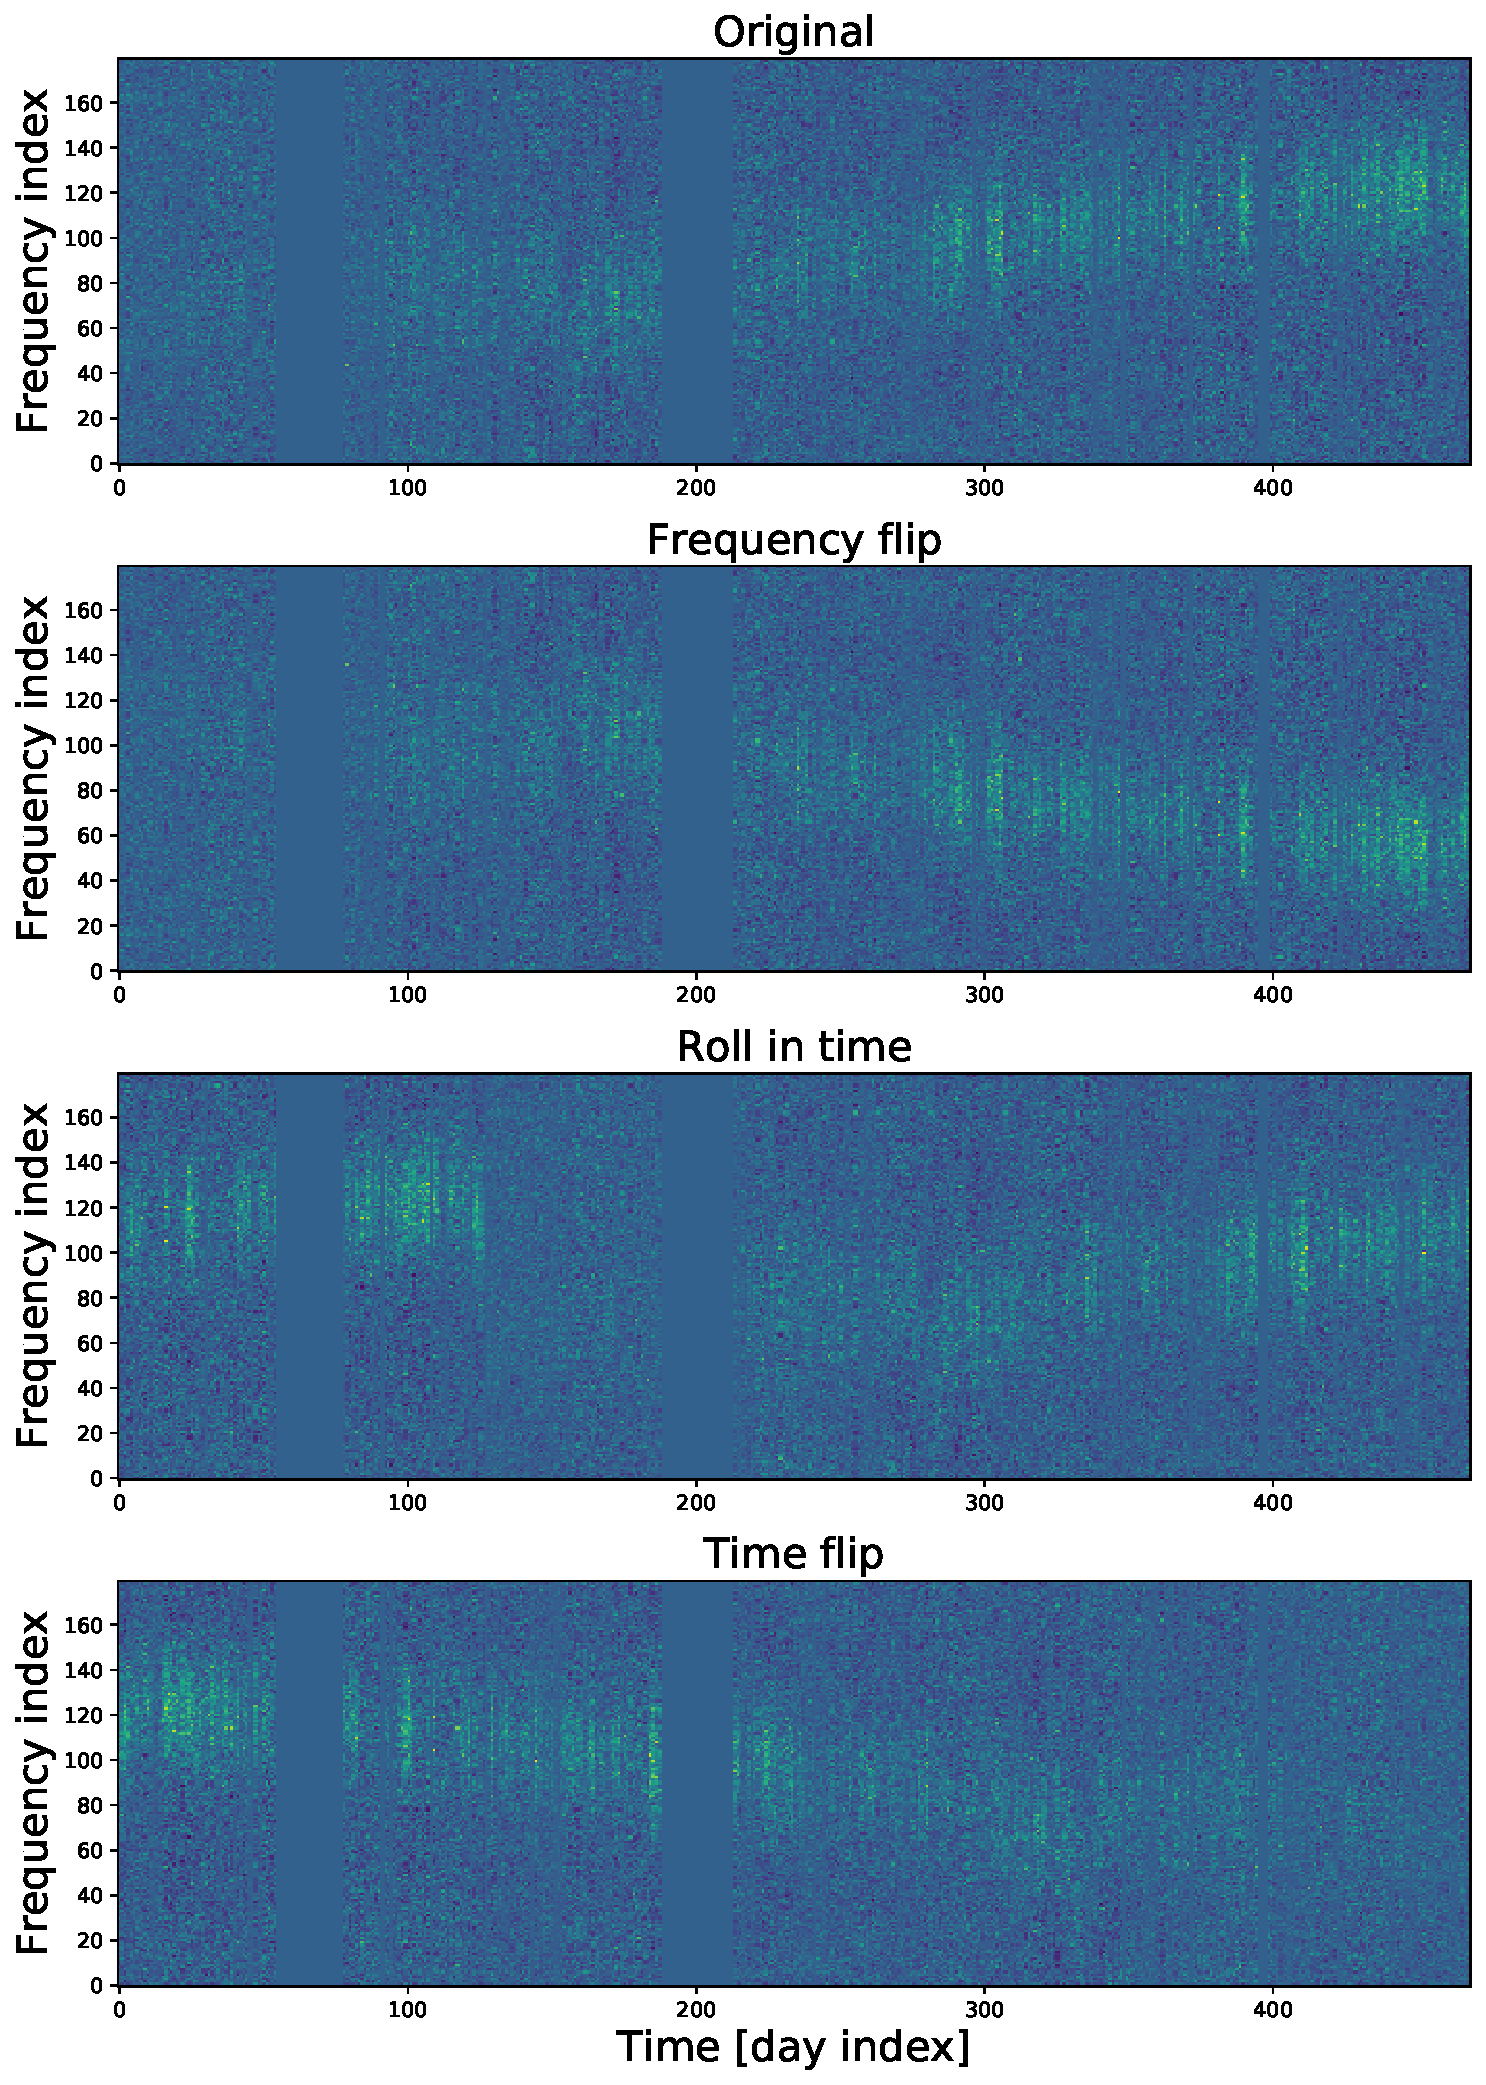
\includegraphics[width=0.7\columnwidth]{C4_cnn/augmentation.pdf}
	\caption{The data is transformed by flipping the data in frequency (panel 2), rolling the data in time by 100 bins (panel 3) and flipping the data in time (panel 4). The original summed spectrogram is show in panel 1. Simulated signals can then be injected using this data as noise. The plots above show a broad wandering line to demonstrate the changes to the data when it is augmented, however, the majority of sub-bands contain almost Gaussian noise. }
	\label{machine:data:augmentation:examples}
\end{figure}

%%%%%%%%%%%%%%%%%%%%%%%%%%%%%%%%%%%%%%%%%%%%%%%%%
\subsection{\label{machine:data:downsample} Downsampling}
%%%%%%%%%%%%%%%%%%%%%%%%%%%%%%%%%%%%%%%%%%%%%%%%%

% introduce downsampling
%
One further issue for our data sets are their size. The spectrograms we use have a large number of pixels within them.
This means that as the spectrograms are passed through the network, there are a large number of computations.
Both this number of computations and the memory requirements of the GPU mean that training a network with a large number of data points takes longer.
We implement a few methods to reduce the size of the data: summing time segments of
spectrograms and down-sampling these summed spectrograms.  

% describe the downsampling in time and frequency
%
The spectrograms are summed over one day, i.e., every 48 time segments, as
in~\cite{bayley2019SOAPGeneralised}. This should increase the \ac{SNR} for a
given signal within a given time-frequency bin assuming that the
signal remains within the frequency bin for the majority of the time segment.
To reduce the size of the data further, the package `resize' from scikit-image
\cite{vanderwalt2014ScikitimageImage} is used, this uses interpolation to
resize the summed spectrograms to a size of (156,89) [time segments,frequency
bins]. This size was defined based on the summed spectrograms of the S6 data-set. This is 1/3 the number of summed segments in time, 1/2 the number of segments in frequency. The down-sampling is applied to the
spectrograms and vitmaps. 
In \cite{bayley2019SOAPGeneralised} we demonstrated that summing spectrograms can increase the speed and sensitivity of our search.
When down-sampling the image, we found that reducing the amount of data had a small affect on the sensitivity of the \acp{CNN} used.

%%%%%%%%%%%%%%%%%%%%%%%%%%%%%
%%%%%%%%%%%%%%%%%%%%%%%%%%%%%
\section{\label{machine:pipeline}Search pipeline}
%%%%%%%%%%%%%%%%%%%%%%%%%%%%%%%%%%%%
%%%%%%%%%%%%%%%%%%%%%%%%%%%%%%%%%

In previous sections each component of the search pipeline has been described,
however, described below is how each component fits together. Fig.~\ref{machine:pipeline:flow} shows a flow diagram of the pipeline. The pipeline is run in three different ways: training the \ac{CNN}, testing the search and running a search on real data. 

\begin{figure}[htp]
	\centering
	\scalebox{0.7}{
	

\tikzstyle{block} = [rectangle, draw, fill=blue!20, 
    text width=17em, text centered, rounded corners, minimum height=4em]
\tikzstyle{line} = [draw,line width=0.35mm, -latex']
\tikzstyle{fillnode} = [rectangle, fill=white, text centered]

\tikzstyle{blocktrain} = [rectangle, draw, fill=red!20, 
    text width=5em, text centered, rounded corners, minimum height=4em]
\tikzstyle{blocktest} = [rectangle, draw, fill=green!20, 
    text width=5em, text centered, rounded corners, minimum height=4em]
\tikzstyle{blocksearch} = [rectangle, draw, fill=black!5, 
    text width=5em, text centered, rounded corners, minimum height=4em]
\tikzstyle{blocktestbig} = [rectangle, draw, fill=green!20, 
    text width=17em, text centered, rounded corners, minimum height=4em]
\tikzstyle{blocksearchbig} = [rectangle, draw, fill=black!5, 
    text width=17em, text centered, rounded corners, minimum height=4em]
\tikzstyle{back group} = [fill=blue!20,rounded corners, draw=black!70, dashed, inner xsep=15pt, inner ysep=7pt, text centered]
\tikzstyle{back group1} = [fill=blue!20,rounded corners, draw=black!70, dashed, inner xsep=15pt, inner ysep=15pt, text centered]


\begin{tikzpicture}[node distance = 6em, auto]

    % Place node
    
  \node [block] (sft) {1.\\ SFTs from Time series};
  
  \node [block, below of=sft] (norm) {2. \\ Divide \ac{SFT} to running median and get power spectrum.};
  \node [block, below of=norm] (narrow) {3. \\ Narrowband \ac{SFT} };
  
  \node [block, below right =1.5cm and -0.9cm of narrow] (odd) {4. \\ Odd.};
  \node [block, below left =1.5cm and -0.9cm of narrow] (even) {4. \\ Even.};
  
  % odd blocks
    
  \node [blocktest,below of= odd] (testodd) {5b.\\ Test data};
  \node [blocktest, below of= testodd] (testsumodd) {6b. \\Test data};
  \node [blocktest, below of=testsumodd] (testlookupodd) {7b. \\ Test data};
  \node [blocktest, below of=testlookupodd] (testdownsampodd) {8b. \\  Test data};
  \node [below of= testdownsampodd](testblankodd) {};
    
  \node [blocktrain, left of= testodd] (trainodd) {5a.\\ Training data};
  \node [blocktrain, below of= trainodd] (trainsumodd) {6a. \\Training data};
  \node [blocktrain, below of=trainsumodd] (trainlookupodd) {7a. \\ Training data};
  \node [blocktrain, below of=trainlookupodd] (traindownsampodd) {8a. \\  Training data};
  \node [blocktrain, below of=traindownsampodd] (trainnetworkodd) {9. \\ Train `odd' \ \ac{CNN}};

  \node [blocksearch,right of=testodd] (searchodd) {5c.\\ Search data};
  \node [blocksearch, below of= searchodd] (searchsumodd) {6c. \\Search data};
  \node [blocksearch, below of=searchsumodd] (searchlookupodd) {7c. \\ Search data};
  \node [blocksearch, below of=searchlookupodd] (searchdownsampodd) {8c. \\  Search data};
  \node [below of= searchdownsampodd](searchblankodd) {};
  
  \node [blocktest, below = 1.4cm of testblankodd] (testclassifyodd) {10b.\\ Test data};
  \node [blocksearch, below = 1.4cm of searchblankodd] (searchclassifyodd) {10c.\\ Search data};

   
  % even blocks]
  
    \node [blocksearch,below of=even] (searcheven) {5c.\\ Search data};
  \node [blocksearch, below of= searcheven] (searchsumeven) {6c. \\Search data};
  \node [blocksearch, below of=searchsumeven] (searchlookupeven) {7c. \\ Search data};
  \node [blocksearch, below of=searchlookupeven] (searchdownsampeven) {8c. \\ Search data};
  \node [below of= searchdownsampeven](searchblankeven) {};
  
  \node [blocktest,left of= searcheven] (testeven) {5b.\\Test data};
  \node [blocktest, below of= testeven] (testsumeven) {6b. \\Test data};
  \node [blocktest, below of= testsumeven] (testlookupeven) {7b. \\Test data};
  \node [blocktest, below of=testlookupeven] (testdownsampeven) {8b. \\ Test data};
  \node [below of= testdownsampeven](testblankeven) {};
  
  \node [blocktrain, right of= searcheven] (traineven) {5a.\\ Training data};
  \node [blocktrain, below of= traineven] (trainsumeven) {6a. Training data};
  \node [blocktrain, below of=trainsumeven] (trainlookupeven) {7a. \\Training data};
  \node [blocktrain, below of=trainlookupeven] (traindownsampeven) {8a. \\ Training data};
  \node [blocktrain, below of=traindownsampeven] (trainnetworkeven) {9. \\ Train `even'  \ \ac{CNN}};

  
  \node [blocktest, below = 1.4cm of testblankeven] (testclassifyeven) {10b.\\ Test data};
  \node [blocksearch, below = 1.4cm of searchblankeven] (searchclassifyeven) {10c.\\ Search data};
  
% background blocks  
  
\begin{scope}[on background layer]
   
    \node (bkgen) [back group] [fit=(trainodd) (testodd) (searchodd) (traineven) (testeven) (searcheven) ] {5.\\Injections};
    
    \node (bksum) [back group] [fit=(trainsumodd) (testsumodd) (searchsumodd) (trainsumeven) (testsumeven) (searchsumeven)] {6.\\Sum spectrograms over \\1 day};
    
    \node (bksoap) [back group] [fit=(trainlookupodd) (testlookupodd) (searchlookupodd) (trainlookupeven) (testlookupeven) (searchlookupeven)] {7.\\Generate lookup tables \\and\\ run SOAP search.};
    
    \node (bkdown) [back group] [fit=(traindownsampodd) (testdownsampodd) (searchdownsampodd) (traindownsampeven) (testdownsampeven) (searchdownsampeven)] {8.\\Downsample spectrograms\\ and vitmaps.};
    
    \node (bkclassodd) [back group1] [fit=(testclassifyodd) (searchclassifyodd)] {};
     
    \node (bkclasseven) [back group1] [fit=(testclassifyeven) (searchclassifyeven)] {};

    
 \end{scope}
 
   % search and testing
  
  \node [blocktestbig, below right =1.1cm and -3.5cm of bkclasseven] (output) {11c.\\ Generate efficiency curves from test data.};
  \node [blocksearchbig, below left= 1.1cm and -3.5cm of bkclassodd] (outputsearch) {11a.\\ Take top 1\% of search bands for followup.};
  
  % Draw edges
  \path [line] (sft) -- (norm);
  \path [line] (norm) -- (narrow);
  
  % even lines
  
   \path [line] (narrow) -- (even);
  
  \path [line] (even) -- (testeven);
  \path [line] (even) -- (traineven);
  \path [line] (even) -- (searcheven);
  
  \path [line,red!60] (traineven) -- (trainsumeven.north);
  \path [line,green!60] (testeven.south) -- (testeven.south|-testsumeven.north);
  \path [line,black!60] (searcheven.south) -- (searcheven.south|-searchsumeven.north);
  
  \path [line,green!60] (testeven.south|-testsumeven.south) -- (testeven.south|-testlookupeven.north);
  \path [line,red!60] (traineven.south|-trainsumeven.south) -- (traineven.south|-trainlookupeven.north);
  \path [line,black!60] (searcheven.south|-searchsumeven.south) -- (searcheven.south|-searchlookupeven.north);
  
  \path [line,green!60] (testeven.south|-testlookupeven.south) -- (testeven.south|-testdownsampeven.north);
  \path [line,red!60] (traineven.south|-trainlookupeven.south) -- (traineven.south|-traindownsampeven.north);
  \path [line,black!60] (searcheven.south|-searchlookupeven.south) -- (searcheven.south|-searchdownsampeven.north);
  
  \path [line,red!60] (traindownsampeven) -- (trainnetworkeven);
  \path [line,green!60] (testdownsampeven) -- (testclassifyeven);
  \path [line,black!60] (searchdownsampeven) -- (searchclassifyeven);
  
  %\path [line,black!60] (searcheven.south|-searchdownsampeven.south) -- (searcheven.south|-classifyeven.north);
  %\path [line,green!60] (testeven.south|-testdownsampeven.south) -- (testeven.south|-classifyeven.north);
  
  \path [line,red!60] (trainnetworkeven) -- (bkclassodd);
  
  %% odd lines
  
   \path [line] (narrow) -- (odd);
  
  \path [line] (odd) -- (testodd);
  \path [line] (odd) -- (trainodd);
  \path [line] (odd) -- (searchodd);
  
  \path [line,red!60] (trainodd) -- (trainsumodd.north);
  \path [line,green!60] (testodd.south) -- (testodd.south|-testsumodd.north);
  \path [line,black!60] (searchodd.south) -- (searchodd.south|-searchsumodd.north);
  
  \path [line,green!60] (testodd.south|-testsumodd.south) -- (testodd.south|-testlookupodd.north);
  \path [line,red!60] (trainodd.south|-trainsumodd.south) -- (trainodd.south|-trainlookupodd.north);
  \path [line,black!60] (searchodd.south|-searchsumodd.south) -- (searchodd.south|-searchlookupodd.north);
  
  \path [line,green!60] (testodd.south|-testlookupodd.south) -- (testodd.south|-testdownsampodd.north);
  \path [line,red!60] (trainodd.south|-trainlookupodd.south) -- (trainodd.south|-traindownsampodd.north);
  \path [line,black!60] (searchodd.south|-searchlookupodd.south) -- (searchodd.south|-searchdownsampodd.north);
  
  \path [line,red!60] (traindownsampodd) -- (trainnetworkodd);
  \path [line,green!60] (testdownsampodd) -- (testclassifyodd);
  \path [line,black!60] (searchdownsampodd) -- (searchclassifyodd);
  
  %\path [line,black!60] (searchodd.south|-searchdownsampodd.south) -- (searchodd.south|-classifyodd.north);
  \%path [line,green!60] (testodd.south|-downsampodd.south) -- (testodd.south|-classifyodd.north);
  
  \path [line,red!60] (trainnetworkodd) -- (bkclasseven);
  
  % search and test
  
  \path [line,green!60] (testclassifyeven) -- (output);
  \path [line,black!60] (searchclassifyeven) -- (outputsearch);
  
  \path [line,green!60] (testclassifyodd) -- (output);
  \path [line,black!60] (searchclassifyodd) -- (outputsearch);
  
  % final labels over lines
  
   \node[fillnode,below] at (bkclasseven.south) {Classify sub-bands with \ `odd' \ac{CNN}};
   
   \node[fillnode,below] at (bkclassodd.south) {Classify sub-bands with \ `even' \ac{CNN}};
 
    
\end{tikzpicture}}
	\caption{\label{machine:pipeline:flow} This diagram shows the SOAP pipeline from start to finish. There are three main sections: Training (red), Testing (green) and Searching (grey) for both the odd and even bands. The blue sections mean that the same operations is done in all cases.}
	
\end{figure}

\begin{description}
	\item[1. \acp{SFT}] Generate 1800s long \acp{SFT} from detector time-series data. For this search these are already generated.
	
	\item[2. Normalising] The \acp{SFT} are then divided by their running median such that their power spectrum has a mean of $\sim 1$. Each spectrogram is then multiplied by 2 such that they are approximately $\chi^{2}$ distributed.
	
	\item[3. Narrowbanding] To improve the computational efficiency of the search the spectrograms are split into 
	$2.1$ Hz wide bands every $2$ Hz,
	i.e. 100.0-102.1, 102.0-104.1 etc.
	This band size was chosen based on the available computational memory at the time.
	
	\item[4. Band splitting]  As a \ac{CNN} should not be trained on the same data that it will be tested on, each of the $0.1$ Hz wide sub-bands are split into `odd' or `even' bands. 
	
	\item[5a. Training data generation] To generate training data the
	process is the same as in Sec.~\ref{data}.  Each of the $0.1$ Hz sub-bands is `augmented' as in Sec.~\ref{machine:data:augmentation}. For each of the augmented bands, the data is duplicated and then signals are injected into them with \acp{SNR} in the range 50-150. This gives us and example for a noise class and a signal class. There are two of these sets, on for `even' bands and one for `odd'.
	
	\item[5b. Test data generation] For test data signals following parameters in Tab.~\ref{machine:data:injections:table} are injected in to 50\% of the $0.1$ Hz sub-bands. These signal have and \ac{SNR} in the range 20-200. Where we have a set for `odd' and a set for `even'.
	
	\item[5c. Search data] This data is generated such that we can search for a real signal. The sub-bands described in part 4 are now overlapping by 0.05 Hz. This means that if there is a signal it should be fully contained within at least one sub-band. There are both `odd' and `even' versions of this search data.
	
	\item[6. Summing spectrogram] As in \cite{bayley2019SOAPGeneralised} the spectrograms are summed over one day, i.e. every 48 time segments of the spectrogram are summed. This is done separately for each of the 6 data-sets (3 for `odd', 3 for `even'). 
	
	\item[7. Generate lookup tables and run SOAP search] Before the SOAP search is run, the line-aware statistic lookup tables need to be generated as in \cite{bayley2019SOAPGeneralised}. Then for each of the 6 data-sets (3 for `odd', 3 for `even') the SOAP search is run separately. 
	
	\item[8. Down-sample data] At this stage there are four elements which are saved for each of the 6 data-sets. The two spectrograms, the Viterbi maps and the Viterbi statistic. The spectrograms and the Viterbi maps are down-sampled to a size of (156x89) using interpolation from scikit-image's resize \cite{vanderwalt2014ScikitimageImage}. This size was chosen based on the S6 \ac{MDC} data-set, where this is 1/3 the length in time and 1/2 the width in frequency of the summed spectrograms.
	
	\item[9. Train Networks] The down-sampled training data is then used to train a \acp{CNN}. One \ac{CNN} is trained on `odd' bands and a different \ac{CNN} with the same structure is trained `even' bands. 
	
	\item[10b. Run search on test data] The trained \acp{CNN} from part 9 are then used to classify each sub-band in the test data with injections, this returns a statistic in $[0,1]$ where 1 represents the probability of a signal. Here the \ac{CNN} trained on the `odd' bands is tested using the `even' bands and vice versa.
	
	\item[10c. Run search on real data] The trained \acp{CNN} from part 9 are then used to classify each sub-band in the search data, this returns a statistic in $[0,1]$ where 1 represents the probability of a signal. Once again the \ac{CNN} trained on the `odd' bands is tested using the `even' bands and vice versa.
	
	\item[11a. Signal candidates] The signals which have a statistic in the top 1\% are taken for a followup investigation. This can be another search, or just a look `by-eye'.
	
	\item[11c. Efficiency curves] The statistics can be plotted against \ac{SNR} to see how the network classified signals with the \ac{SNR} of the injection. Then the efficiency curves can be generated, this is described in further detail in Sec.~\ref{machine:results:sensitivity} .
	
	
	
\end{description}


%%%%%%%%%%%%%%%%%%%%%%%%%%%%
%%%%%%%%%%%%%%%%%%%%%%%%%%%%
\section{\label{machine:results}Results}
%%%%%%%%%%%%%%%%%%%%%%%%%%%%
%%%%%%%%%%%%%%%%%%%%%%%%%%%%

The networks described in Sec.~\ref{machine:cnn:networks} were trained and tested on four different data-sets: the S6 \ac{MDC} as in \cite{bayley2019SOAPGeneralised,walsh2016ComparisonMethods}, our own injections into O2 data and Gaussian noise which had the same gaps and noise floor as the S6 data-set, and our own injections into real S6 data. 
Each of the searches use training and test data in the frequency range of 100-400 Hz, except the S6 \ac{MDC} which uses data in the range 40-500 Hz for testing and training. 


\subsection{\label{machine:results:sensitivity} Sensitivity}

To investigate the sensitivity of the pipeline we use two measures: the sensitivity depth $\mathcal{D}$ \cite{prix2007SearchContinuous} and optimal \ac{SNR} $\rho$ \cite{behnke2015PostprocessingMethods} which are both defined in \cite{bayley2019SOAPGeneralised} as,
%
\begin{equation}
\label{sigmoid}
\mathcal{D}(f) = \frac{\sqrt{S_h(f)}}{h_0},
\end{equation}
%
where $S_h(f)$ is the single-sided noise \ac{PSD} and $h_0$ is the \ac{GW} amplitude. The optimal \ac{SNR} is defined as,
%
\begin{equation}
\rho^2 = \sum_X 4
\Re\int^{\infty}_{0}\frac{\tilde{h}^X(f)\tilde{h}^{X*}(f)}{S^X(f)}df,
\end{equation}
%
where $X$ indexes the detectors and $\tilde{h}(f)$ is the Fourier transform of the time series of the signal $h(t)$. 
This expression is defined in~\cite{prix2007SearchContinuous} for a double-sided \ac{PSD} and we have defined it for the more common single-sided case.

The sensitivity curves shown in Fig.~\ref{results:o2},\ref{results:s6gauss} and \ref{results:s6mdc} were generated using a $1\%$ false alarm rate, where the false alarm is the value where $1\%$ of bands which do not contain an injection exceed the false alarm. 
This is then used as a detection threshold, such that the statistics for each band which exceed this threshold are converted to a 1 and all that do not to a 0.
From this point we use a window to estimate the efficiency curve for each \ac{SNR}, this follows,
\begin{equation}
y(x) = \frac{\sum_i b_i \mathcal{G}(x_i - x,2)}{\sum_i \mathcal{G}(x_i - x,2)},
\end{equation}
where $b_i$ is the binomial data where $b_i=1$ when the statistic is above the $1\%$ false alarm value, $x_i$ is the \ac{SNR} of point $b_i$, $x$ is the current location in \ac{SNR} and $\mathcal{G}(x_i - x,2)$ is a Gaussian with a mean of the current \ac{SNR} and a standard deviation of 2.
The efficiency curves for each of the described data-sets are shown in Figs.~\ref{results:o2},\ref{results:s6gauss} and \ref{results:s6mdc}.


%%%%%%%%
\subsubsection{O1}
%%%%%%%%%%

For the first test, injections were made into the O1 data-set as in Sec.~\ref{data} between 100 Hz and 400 Hz. Then each of the 6 networks described in Sec.~\ref{cnn:networks} were trained and tested on this data. 
Fig.~\ref{machine:results:o1} shows the sensitivity curves for this test for both \ac{SNR} and sensitivity depth for each of the 6 networks. Focusing on Fig.~\ref{machine:results:snr_o1}, the least sensitive, i.e. furthest to the right, of the \acp{CNN} is the Viterbi statistic (vitstat), this is expected as we know that the Viterbi statistic is sensitive to instrumental lines. 
The spectrogram \ac{CNN} has an improved sensitivity over the Viterbi statistic, this importantly does not involve the SOAP search but is run entirely on down-sampled and summed spectrograms. 
Whilst this network is approaching the most sensitive of the examples in Fig.~\ref{results:o2}, and with further efforts may reach it, this network takes $\sim10$ times the amount of training time. This will be explained in more detail in Sec.~\ref{results:timing}.
The remaining networks achieved almost the same sensitivity. 
The vitmap network however, is the fastest of these to train and is used as an input for all of these remaining networks.
For the O1 data-set we show that with a false alarm of 1\% the Viterbi map \ac{CNN} achieves a sensitivity of SNR $~73$ and sensitivity depth of $~12\; {\rm Hz}^{-1/2}$ with 95\% efficiency.
The \ac{SNR} here should not be compared between different runs as this is the integrated `Recovered' \ac{SNR}. Therefore, observing runs, such as O1, which were shorted will appear to have a greater sensitivity when they in fact do not. 

\begin{figure}
	%\centering
	\begin{subfigure}[h]{0.5\textwidth}
		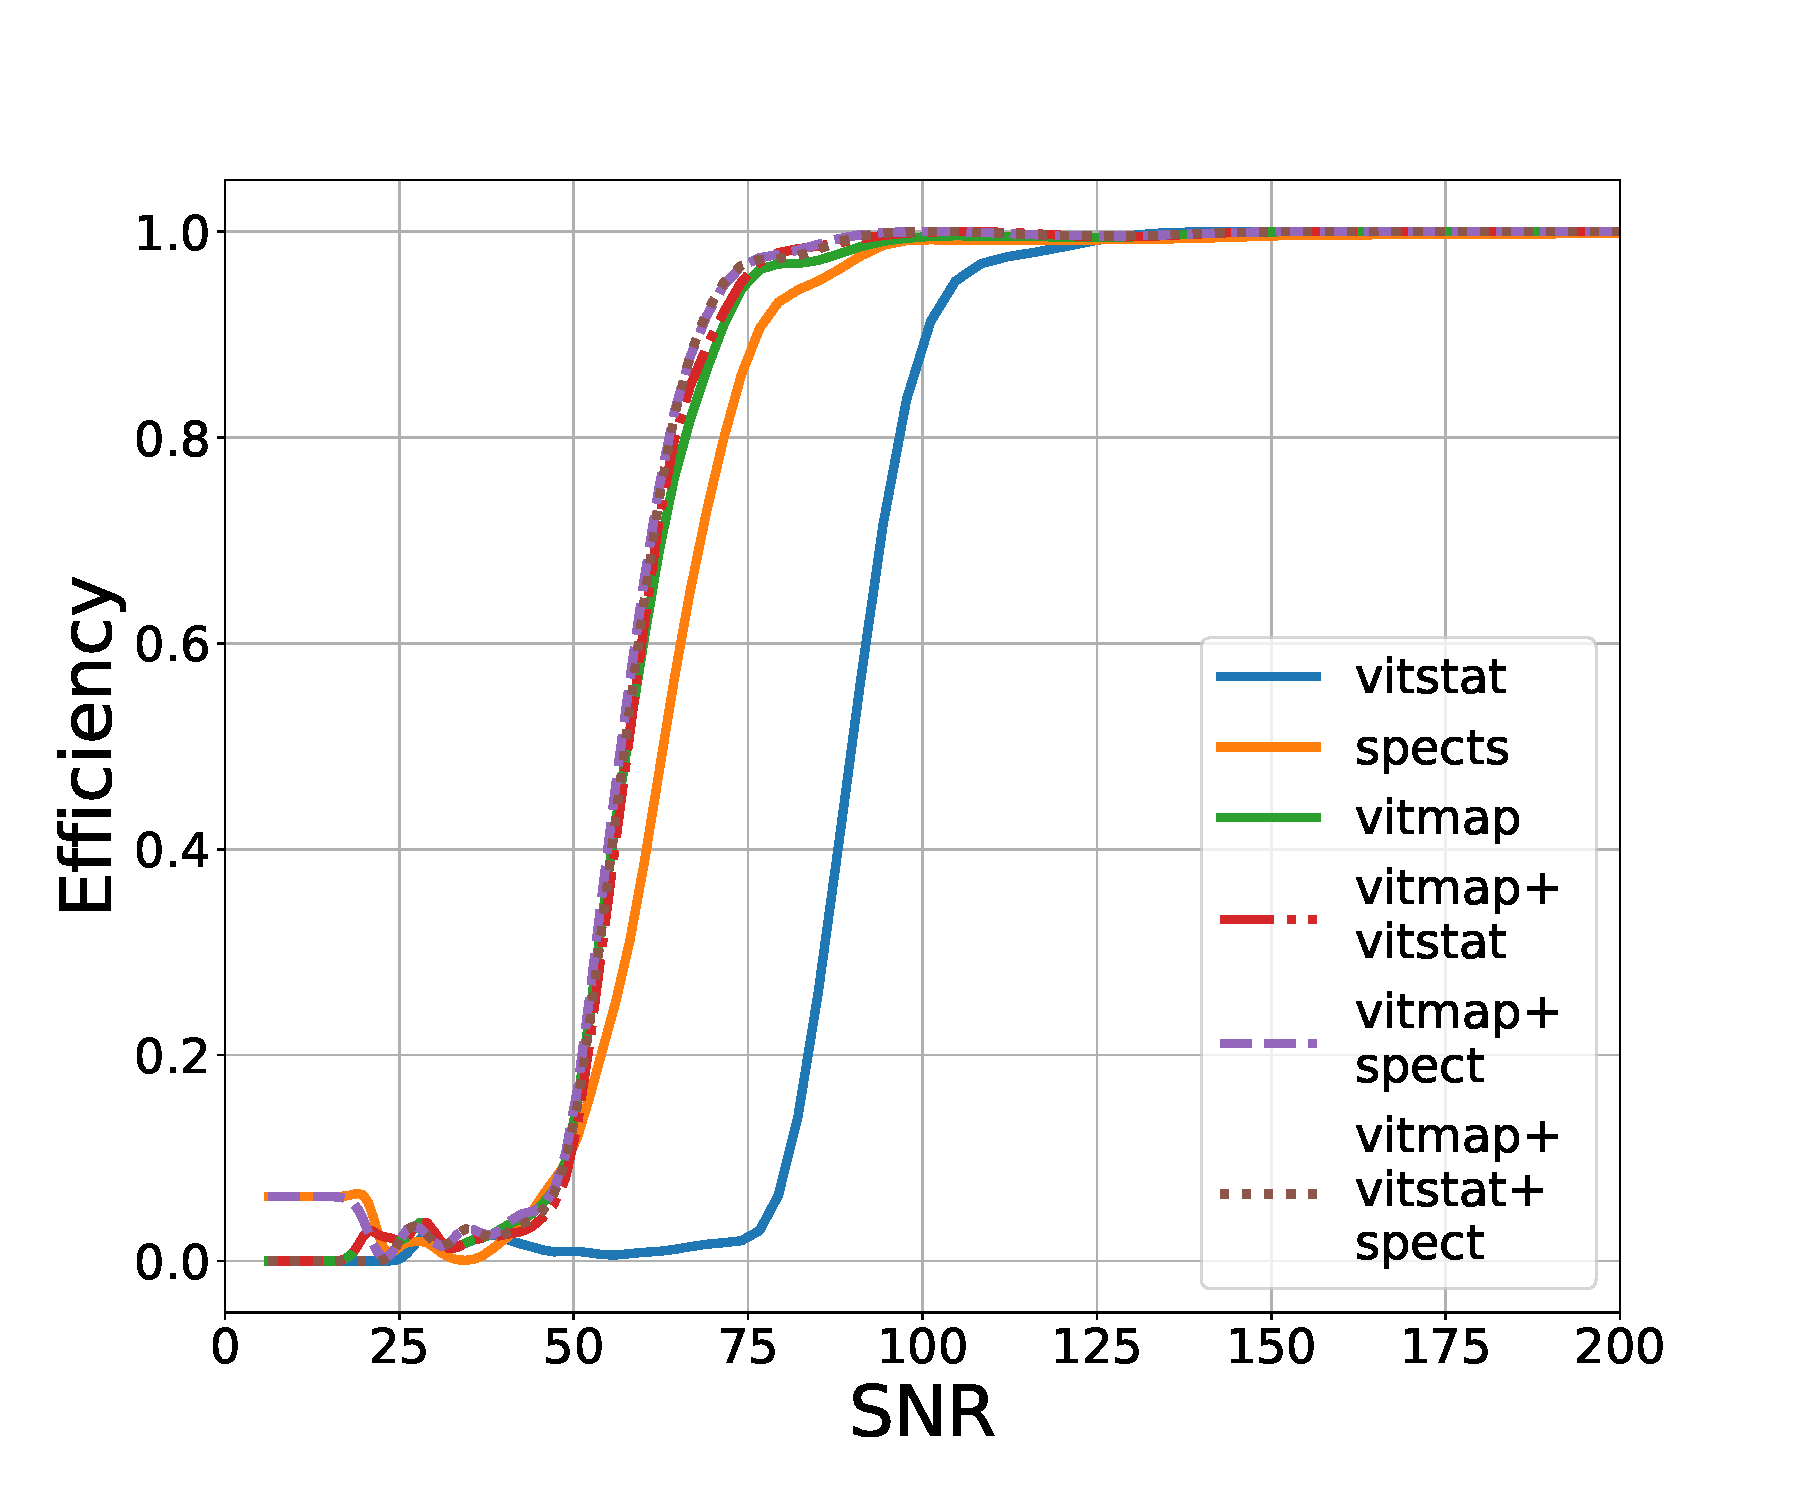
\includegraphics[width=\columnwidth]{C4_cnn/o1_snr_eff.pdf}
		\label{machineresults:snr_o1}
	\end{subfigure}
	\begin{subfigure}[h]{0.5\textwidth}
		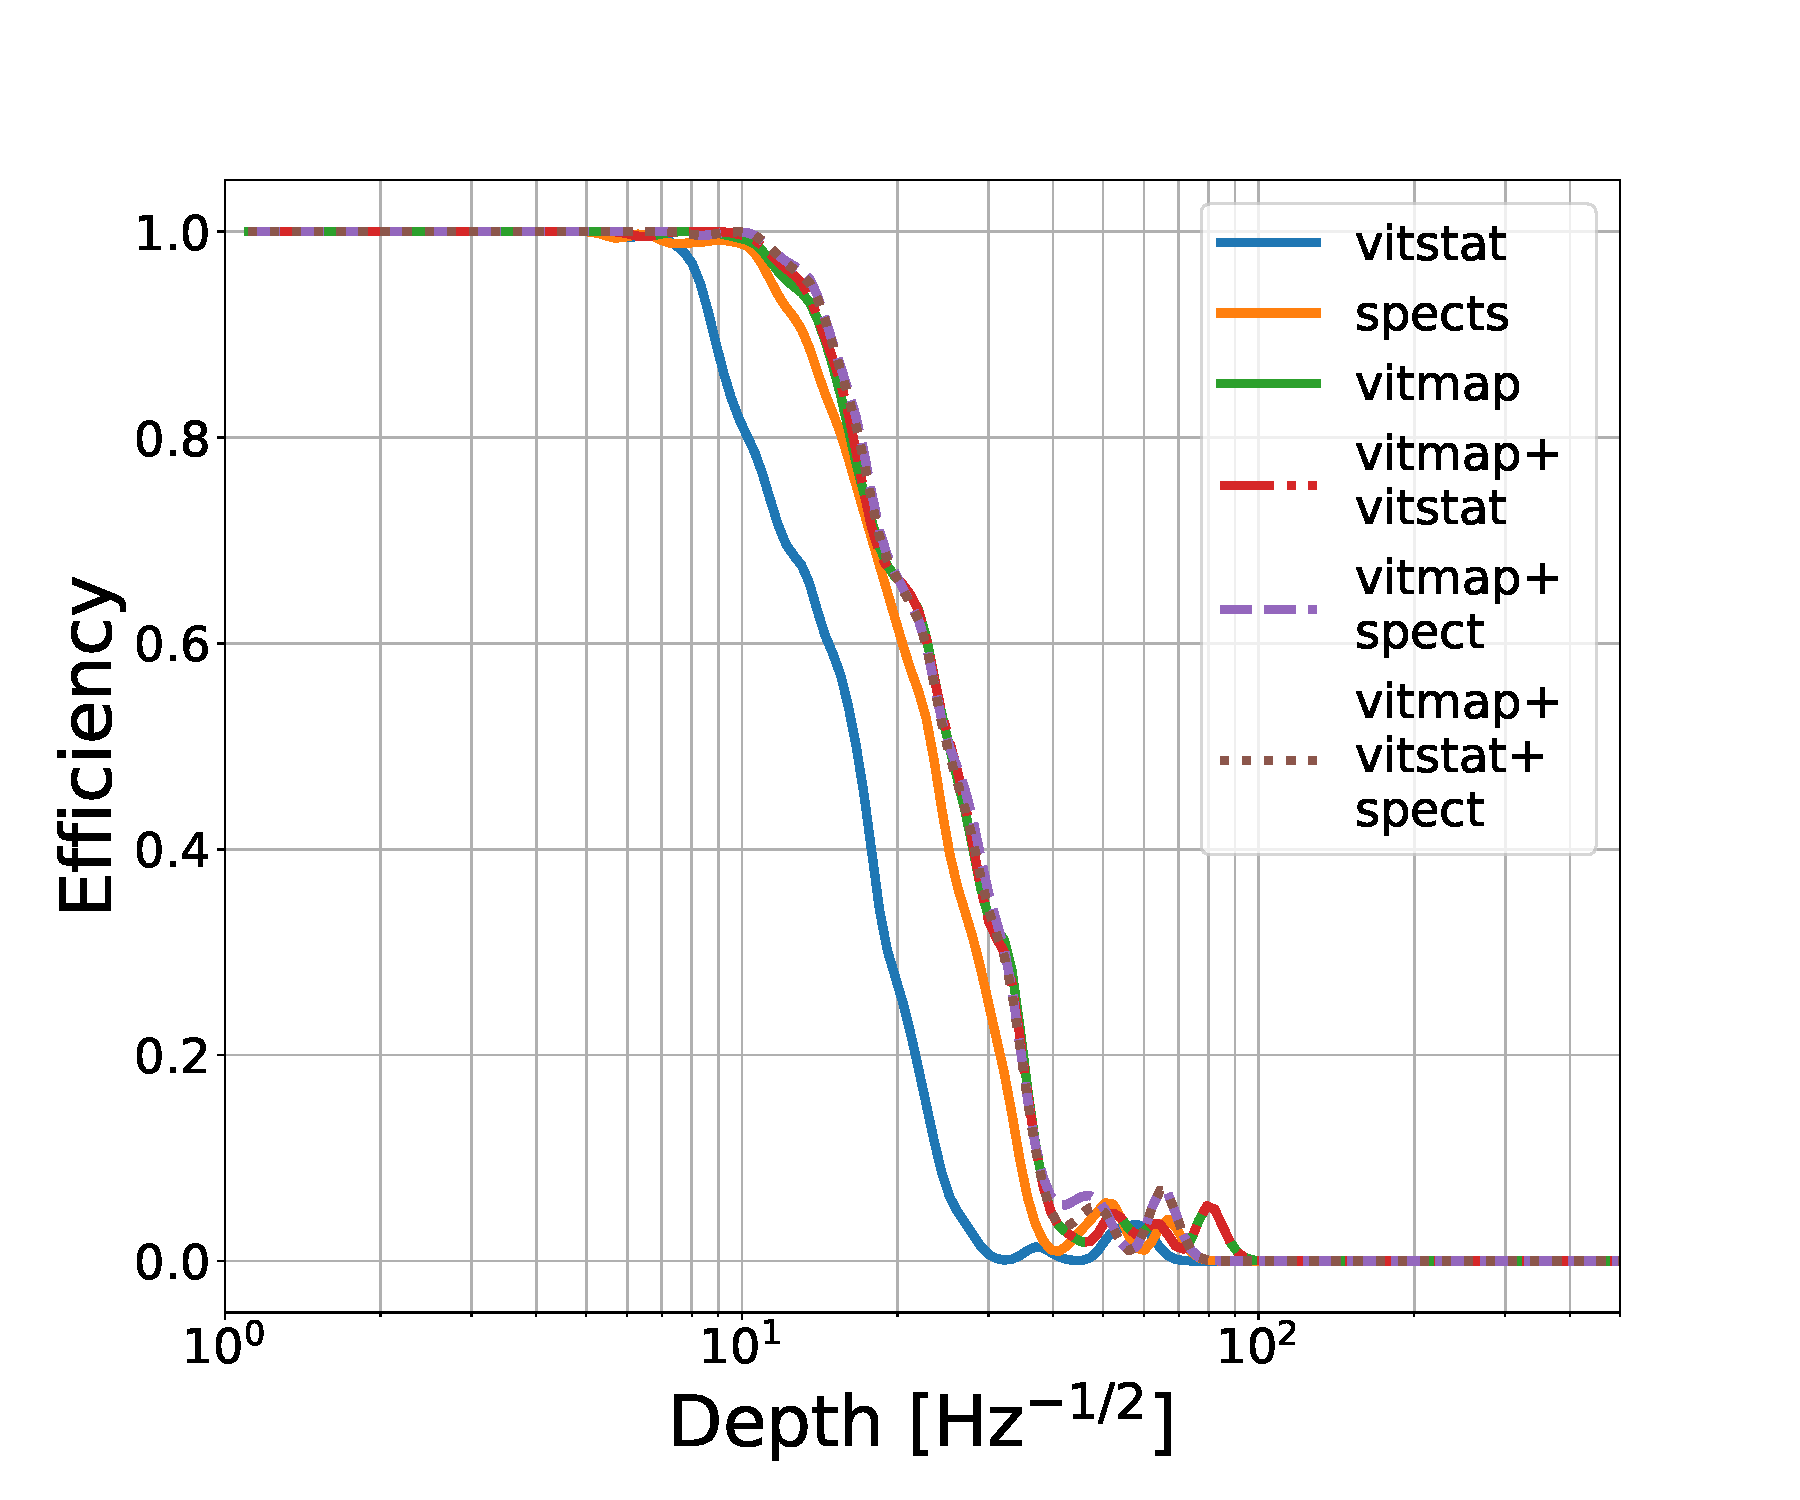
\includegraphics[width=\columnwidth]{C4_cnn/o1_depth_eff.pdf}
		\label{machine:results:depth_o1}
	\end{subfigure}
	\caption{\label{machine:results:o1} In the O1 data-set, each of the six \acp{CNN} were tested. The efficiency plots above are for a 1\% false alarm rate.  }
	
\end{figure}

%%%%%%%%%
\subsubsection{O2}
%%%%%%%%%%

For the next test, injections were made into the O2 data-set in the same way as in the last section. Then each of the 6 networks described in Sec.~\ref{cnn:networks} were trained and tested on this data. 
Fig.~\ref{machine:results:o2} shows the sensitivity curves for this test for both \ac{SNR} and sensitivity depth for each of the 6 networks.
The results here are very similar to the results from the O1 simulations.
The Viterbi statistic is the least sensitive `network', followed by the spectrogram \ac{CNN}.
The remaining four networks all achieve a similar sensitivity, each of these remaining networks contain the Viterbi map as one of their inputs. Therefore, it is assumed that the dominating effect on the sensitivity originated from the Viterbi maps. In following tests the focus will be with the Viterbi map \ac{CNN} as in all cases this is among the most sensitive.
For the O2 data-set we show that with a false alarm of 1\% the Viterbi map \ac{CNN} achieves a sensitivity of SNR $~95$ and sensitivity depth of $~12\; {\rm Hz}^{-1/2}$ with 95\% efficiency.
This result in the sensitivity depth in Fig.~\ref{machine:results:depth_o2} does not vary much from the results from O1, Fig.~\ref{machine:results:depth_o1}. 
Whilst one might expect the sensitivity to increase due to the increase in sensitivity and longer observing run.
However, this is not the case \joe{why?}.

\begin{figure}
	%\centering
	\begin{subfigure}[h]{0.5\textwidth}
		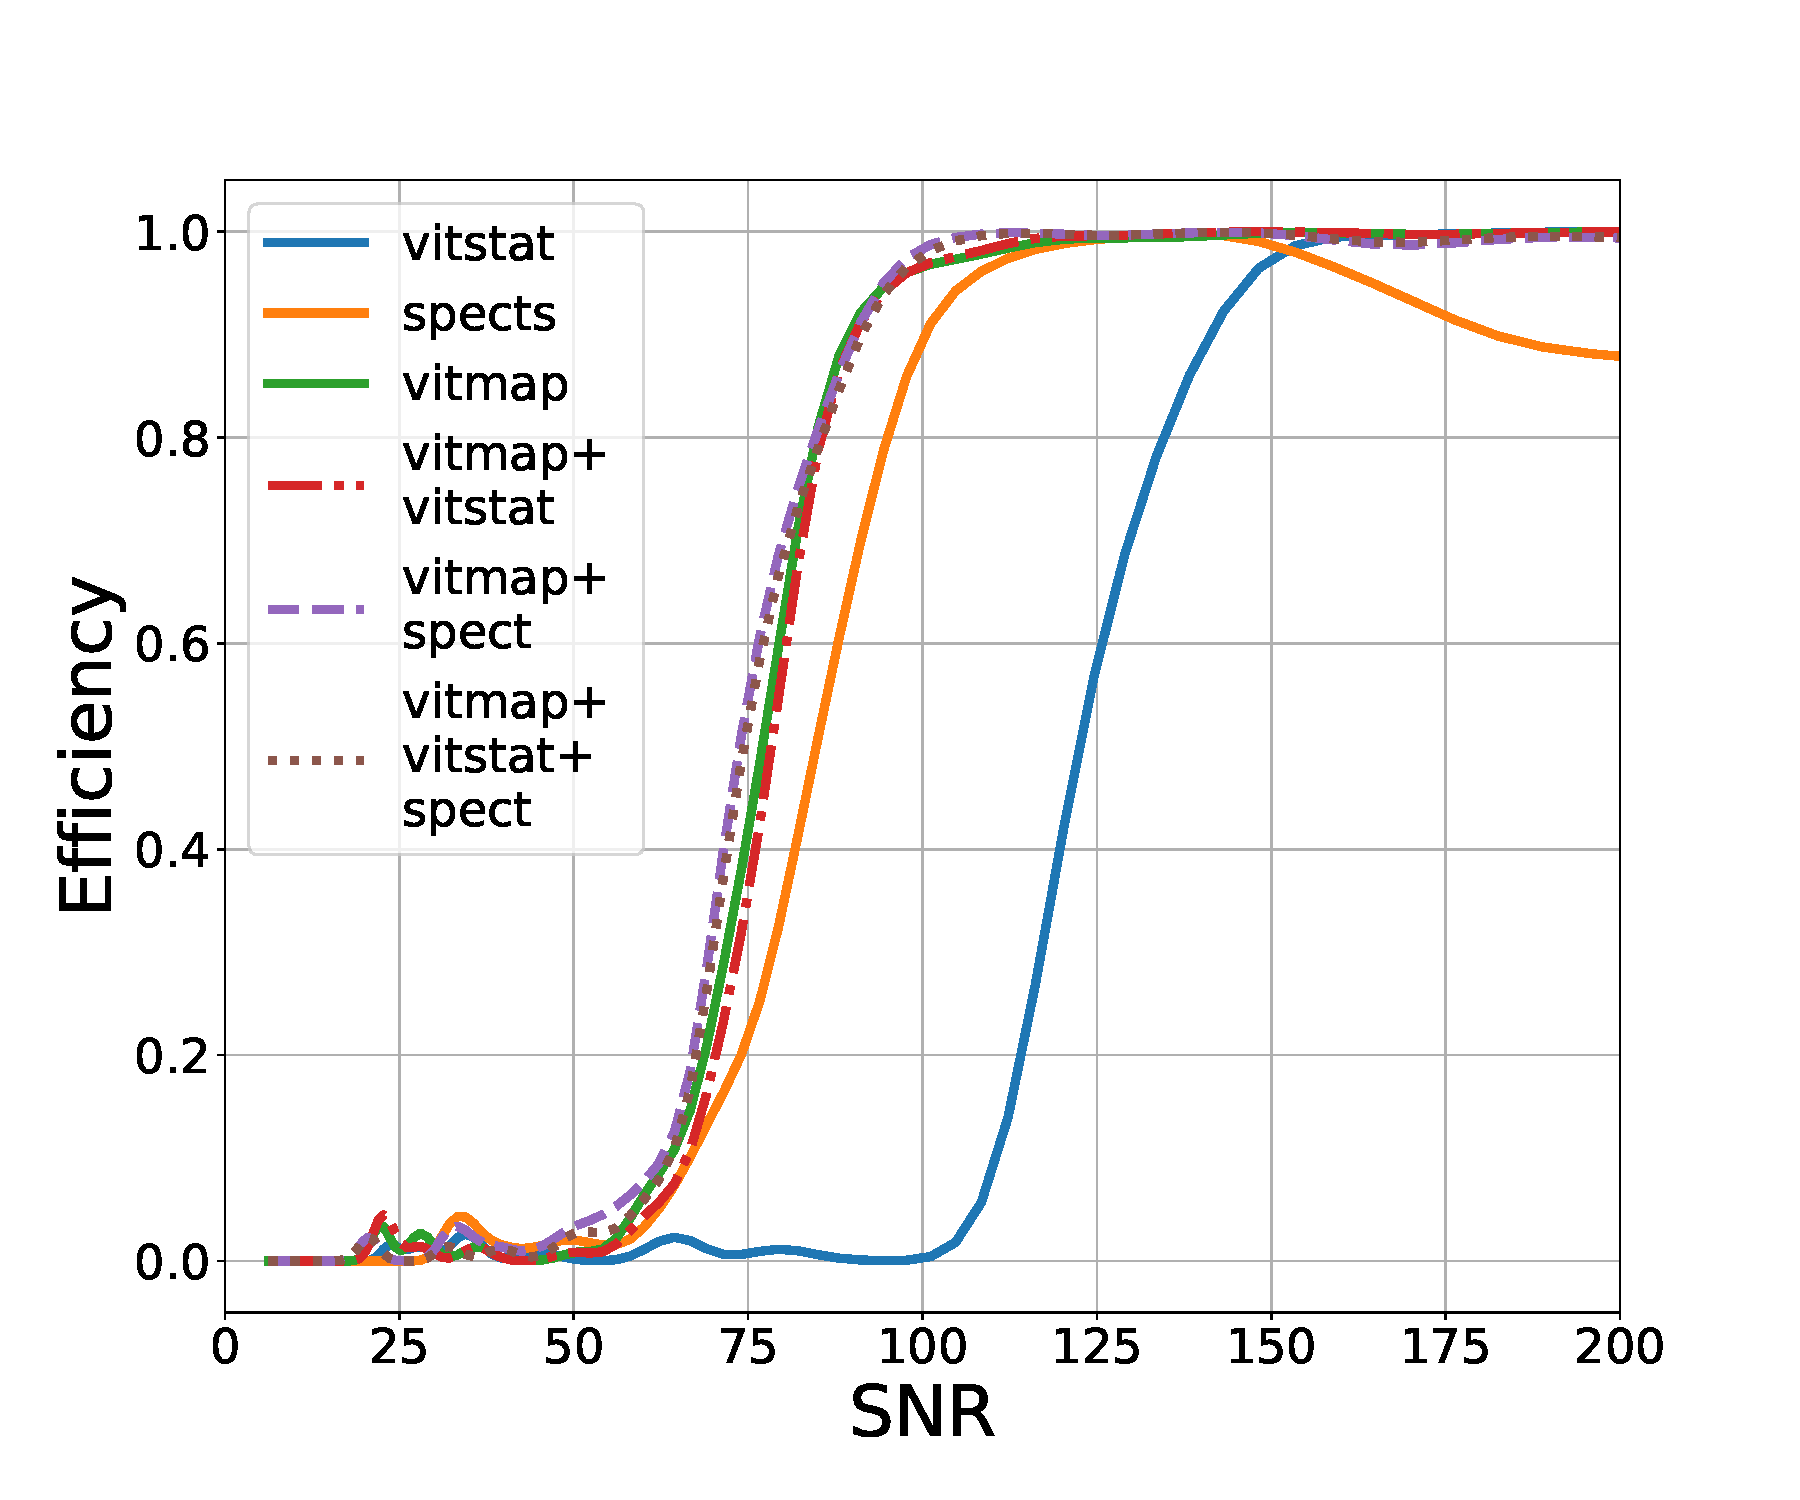
\includegraphics[width=\columnwidth]{C4_cnn/o2_snr_eff.pdf}
		\label{machine:results:snr_o2}
	\end{subfigure}
	\begin{subfigure}[h]{0.5\textwidth}
		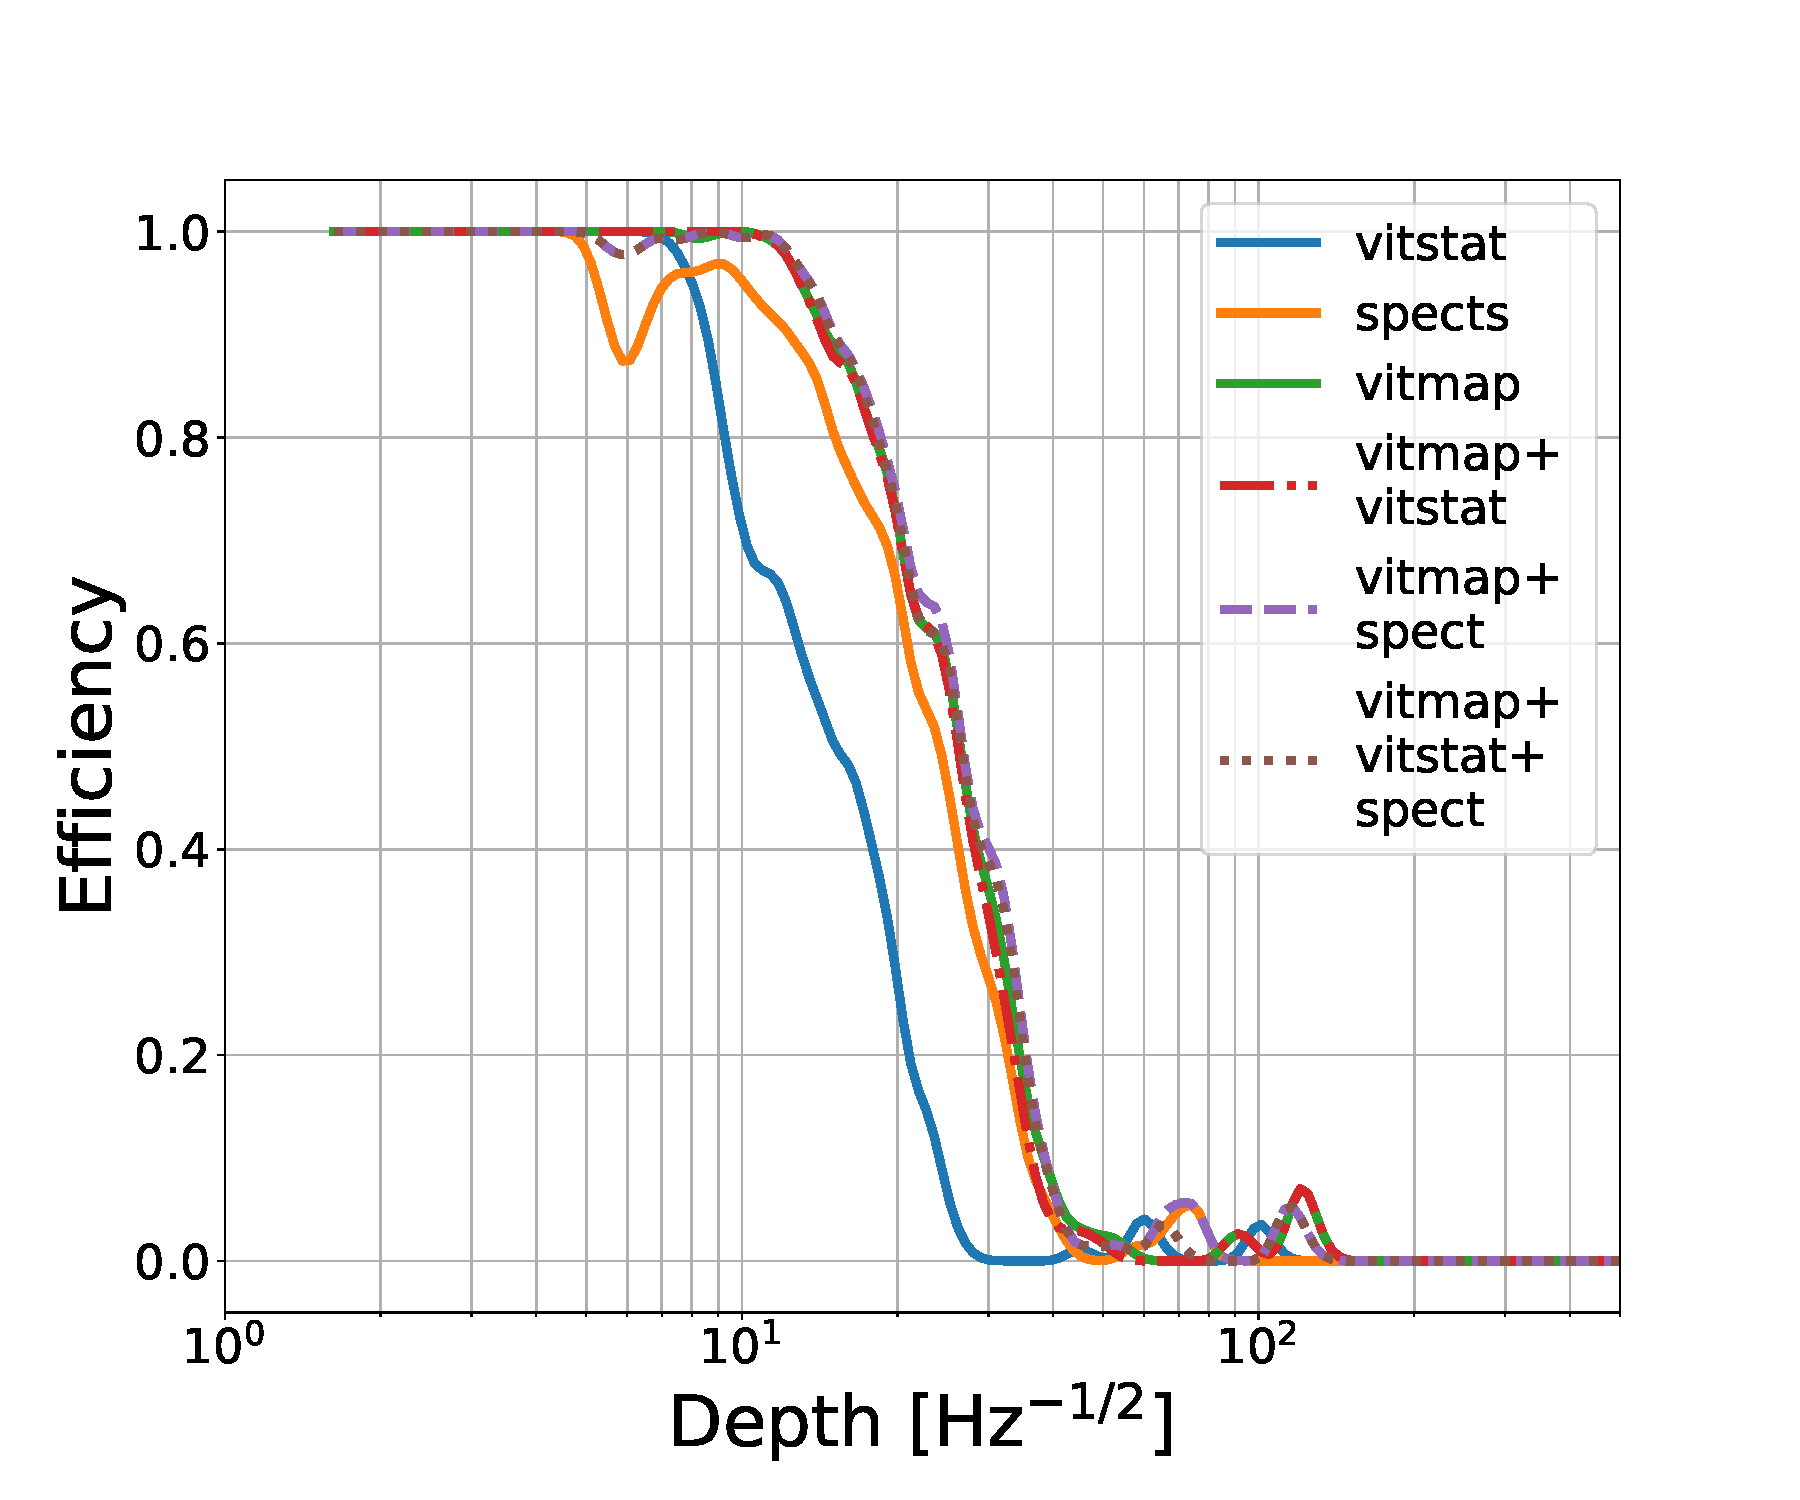
\includegraphics[width=\columnwidth]{C4_cnn/o2_depth_eff.pdf}
		\label{machine:results:depth_o2}
	\end{subfigure}
	\caption{\label{machine:results:o2} In the O2 data-set, each of the six \acp{CNN} were tested. The efficiency plots above are for a 1\% false alarm rate. These show that the use of spectrograms and the Viterbi maps with \acp{CNN} greatly improve the sensitivity when compared to the Viterbi statistic. For each \ac{CNN} which uses a combination of inputs it achieves a similar sensitivity to the \ac{CNN} which uses just the Viterbi map. This implies that the Viterbi map contains the most information out of the tested \acp{CNN}. }
	
\end{figure}



%%%%%%%%%
\subsubsection{Gaussian noise}
%%%%%%%%%%%

The next test involves using injections into Gaussian noise. For this test we tried to replicate the S6 data-set without including instrumental artefacts such as lines. We included the same gaps in data as S6 and the noise floor of S6 was replicated by scaling the \ac{SNR} of any injection in any given \ac{SFT}. 
Fig.~\ref{machine:results:s6gauss} shows the sensitivity curves for the Viterbi statistic and Viterbi map \ac{CNN} for both the Gaussian noise run with S6 gaps and for injections into the S6 data-set. 
In the Gaussian noise data-set the curves for both statistics, Viterbi map and the Viterbi statistic, show very similar results, this is to be expected as the main use of the \ac{CNN} was to reduce the effect of instrumental lines, for which there is none in this data set. 
The advantage of using the Viterbi maps in a \ac{CNN} becomes clear which it is tested on injections into real data with many instrumental lines. 
The remaining curves in Fig.~\ref{machine:results:s6gauss} show these tests, and it becomes clear that the Viterbi map \ac{CNN} reduces the effect of instrumental lines and therefore increases the searches sensitivity. 
These tests in S6 also show that the effect of instrumental lines was far greater in this run than in O2. 
This is shown in Fig.~\ref{machine:results:o2} where the separation between the Viterbi statistic curves and the Viterbi map curves is much smaller than the S6 curves in Fig.~\ref{machine:results:s6gauss}.
For injections into Gaussian noise following S6 gaps we show that with a false alarm of 1\% the Viterbi map \ac{CNN} achieves a sensitivity of SNR $~85$ and sensitivity depth of $~20\; {\rm Hz}^{-1/2}$ with 95\% efficiency. For injections into real S6 data the search achieves a sensitivity of SNR $~115$ and sensitivity depth of $~11\; {\rm Hz}^{-1/2}$ with 95\% efficiency and 1\% false alarm. We can also see from Fig.~\ref{machine:results:s6gauss} that the sensitivity in Gaussian noise with S6 gaps is better than in real S6 data, so there are still some elements of the search which reduces the sensitivity.

\begin{figure}
	\begin{subfigure}[h]{0.5\textwidth}
		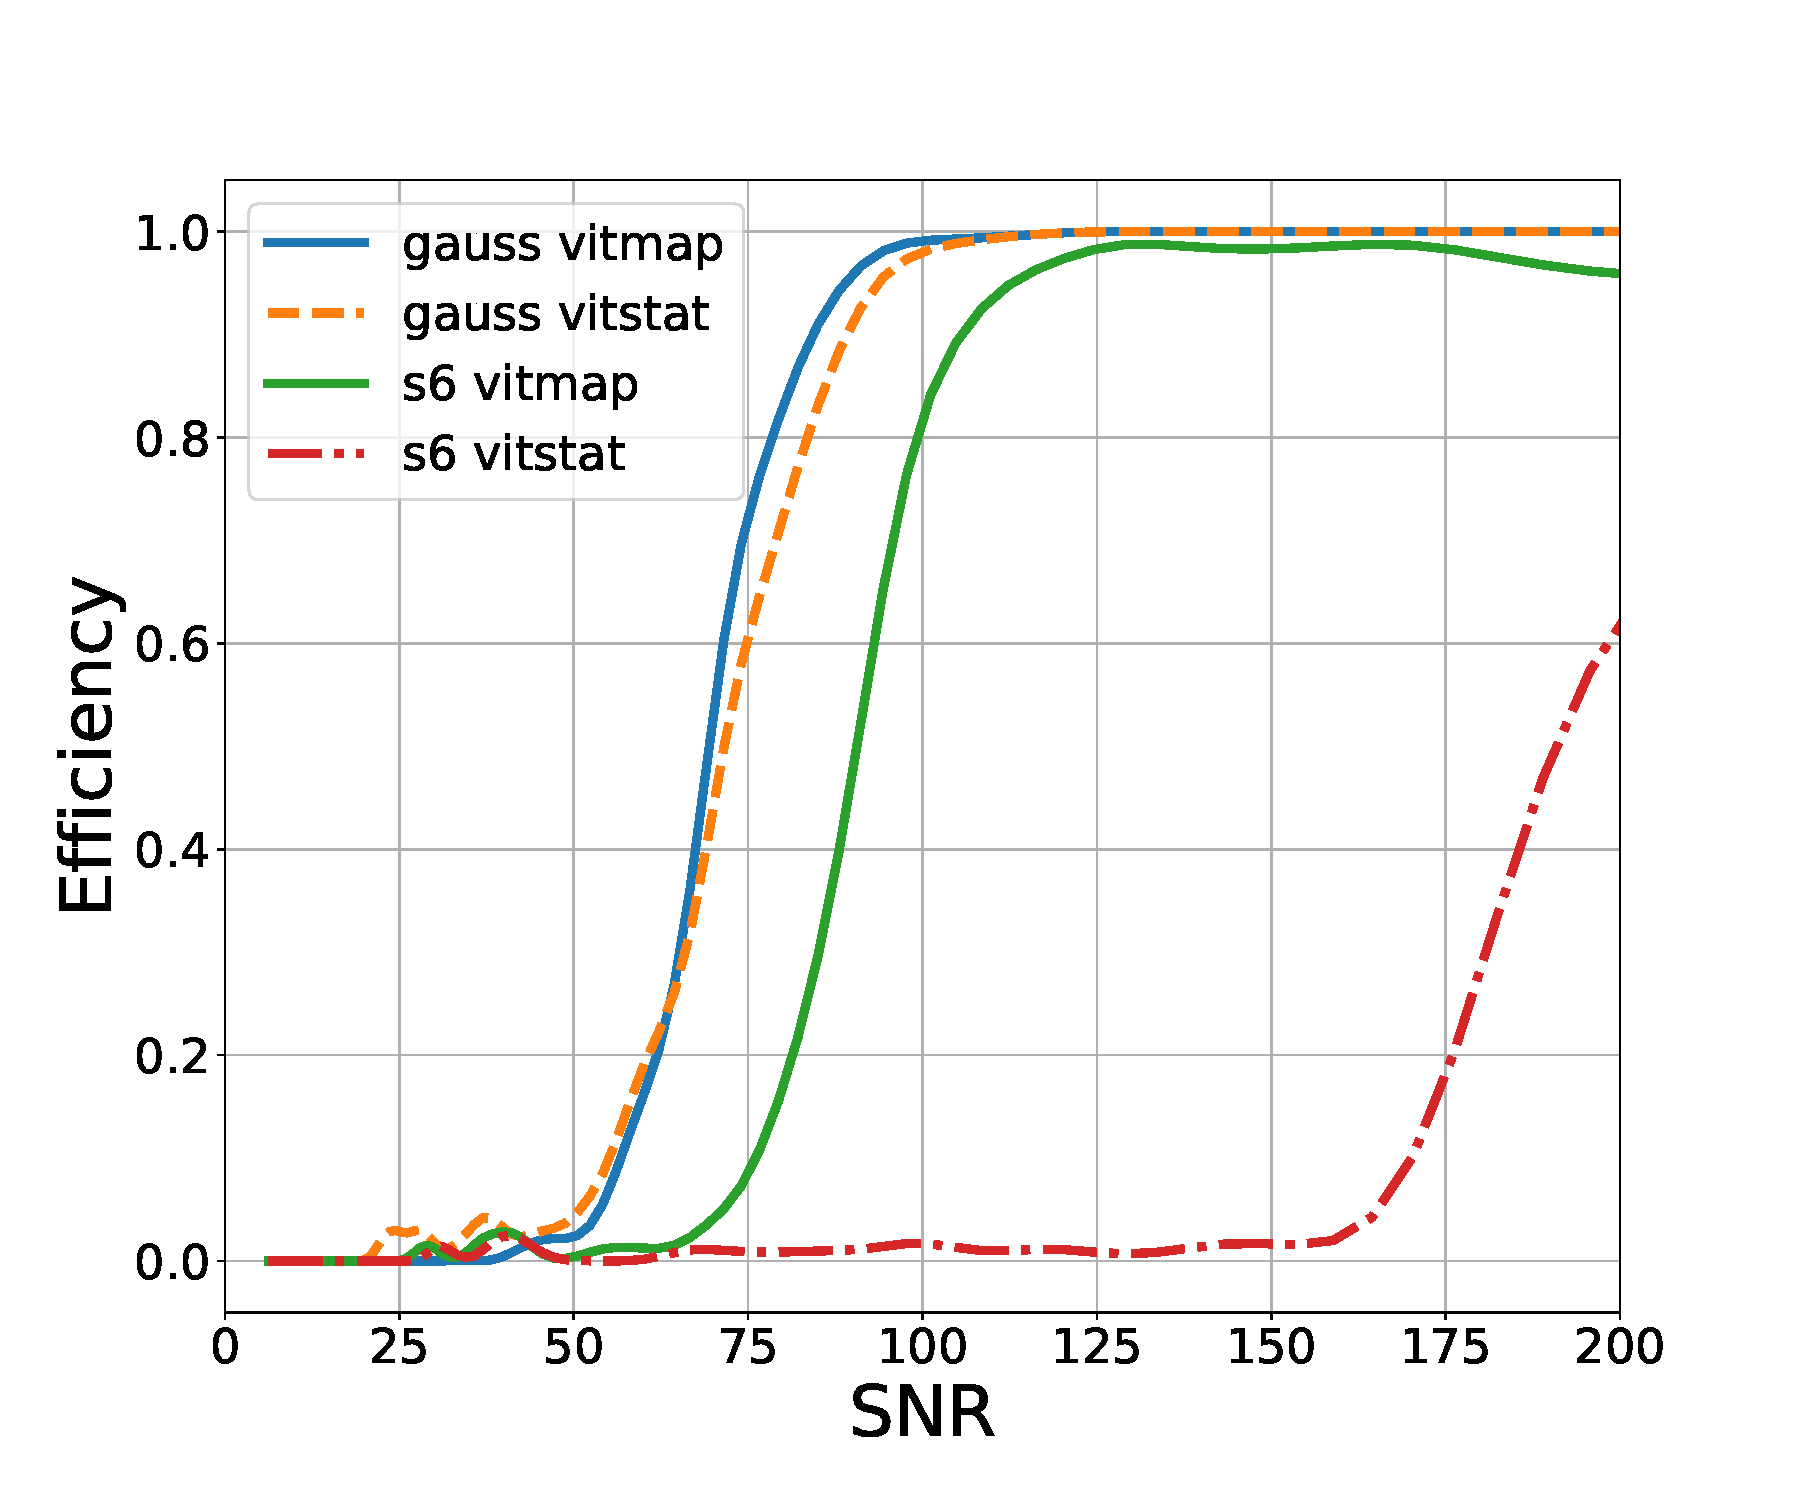
\includegraphics[width=\columnwidth]{C4_cnn/gauss_and_s6_snr_eff.pdf}
		\label{machine:results:snr_s6}
	\end{subfigure}
	\begin{subfigure}[h]{0.5\textwidth}
		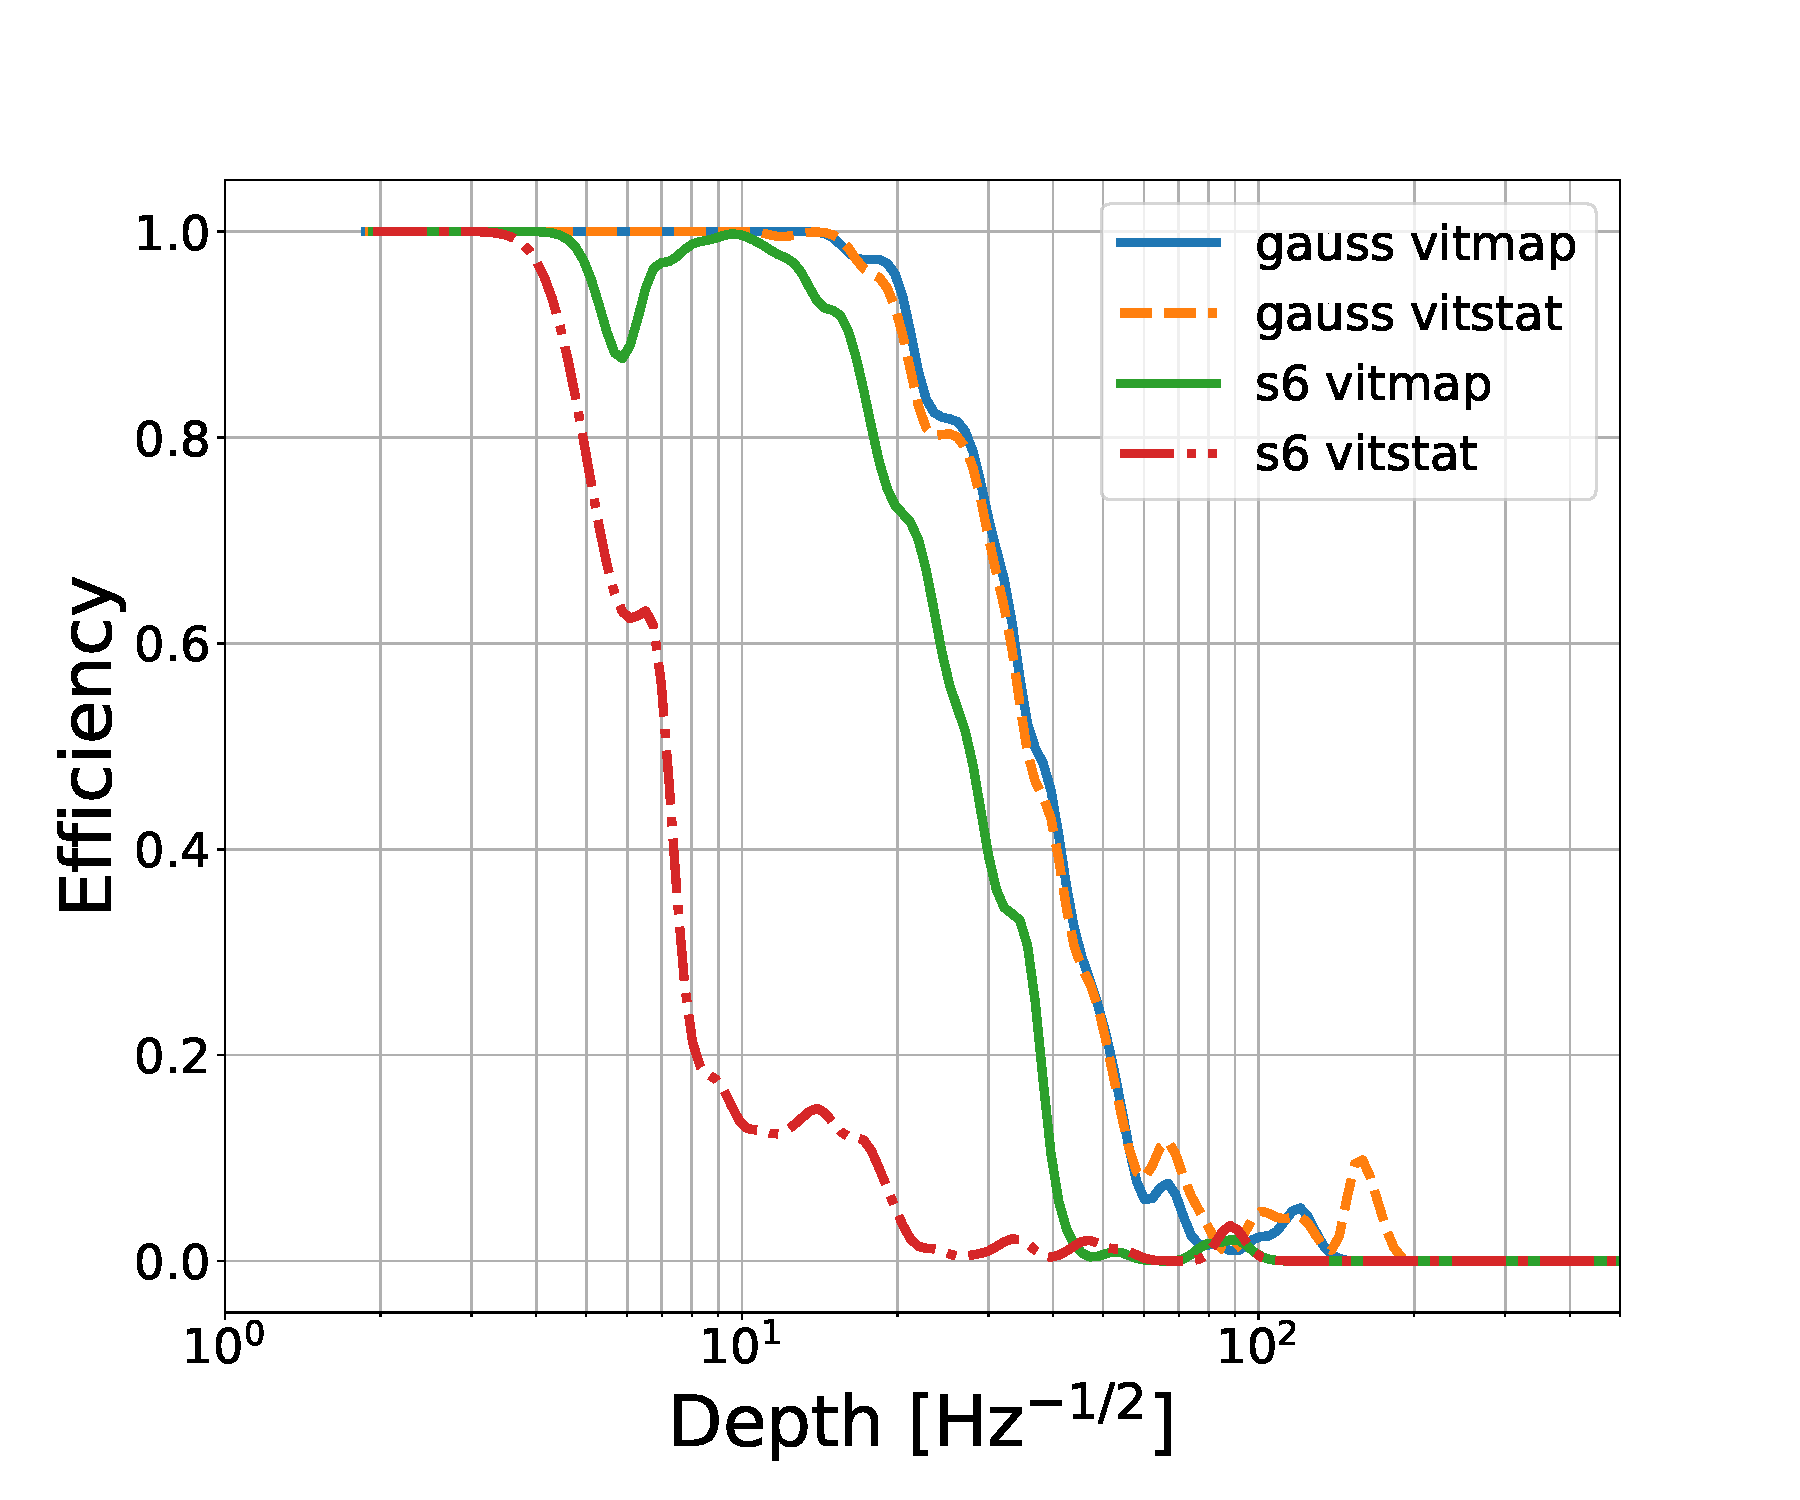
\includegraphics[width=\columnwidth]{C4_cnn/gauss_and_s6_depth_eff.pdf}
		\label{machine:results:depth_s6}
	\end{subfigure}

	\caption{\label{machine:results:s6gauss} We aimed to compare the sensitivity of this search on simulations on real data (s6) to simulations in Gaussian noise (gauss). The Gaussian noise injections included the same gaps in data as the S6 data set. The \ac{SNR} of the simulated signal in Gaussian noise was adjusted based on the noise floor of S6. The sensitivity curves show that the Viterbi map \ac{CNN} (vitmap)achieves a similar sensitivity to the Viterbi statistic (vitstat) in Gaussian noise. This is because the main factor which effects the sensitivity of the Viterbi statistic is instrumental lines. As expected in real data, the Viterbi statistic is far less sensitive. The power of the \ac{CNN} becomes clear in tests on real data. The sensitivity of the Viterbi map \ac{CNN} is improved by over a factor of 2 in \ac{SNR} when tested on S6 data.}
	
\end{figure}

%%%%%%%
\subsubsection{S6}
%%%%%%%%%%

The final test was set up to again use the S6 data-set, however, we use a standard set of injections in the S6 \ac{MDC} \cite{walsh2016ComparisonMethods} to compare directly to other \ac{CW} search pipelines. In Fig.~\ref{machine:results:s6mdc} we show the results of the sensitivity curves from these injections. Fig.~\ref{machine:results:mdccomp} shows the direct comparison in depth of the results in \cite{walsh2016ComparisonMethods} with the results from the SOAP search with the Viterbi map \ac{CNN}. This shows that we achieve a sensitivity similar to many other semi-coherent searches with the exception of the Einstein@home search \cite{abbott2016ResultsDeepest}. For tests in the S6 \ac{MDC} we show that with a false alarm of 1\% the Viterbi map \ac{CNN} achieves a sensitivity of SNR $~90$ and sensitivity depth of $~16\; {\rm Hz}^{-1/2}$ with 95\% efficiency.


\begin{figure}
	\begin{subfigure}[h]{0.5\textwidth}
		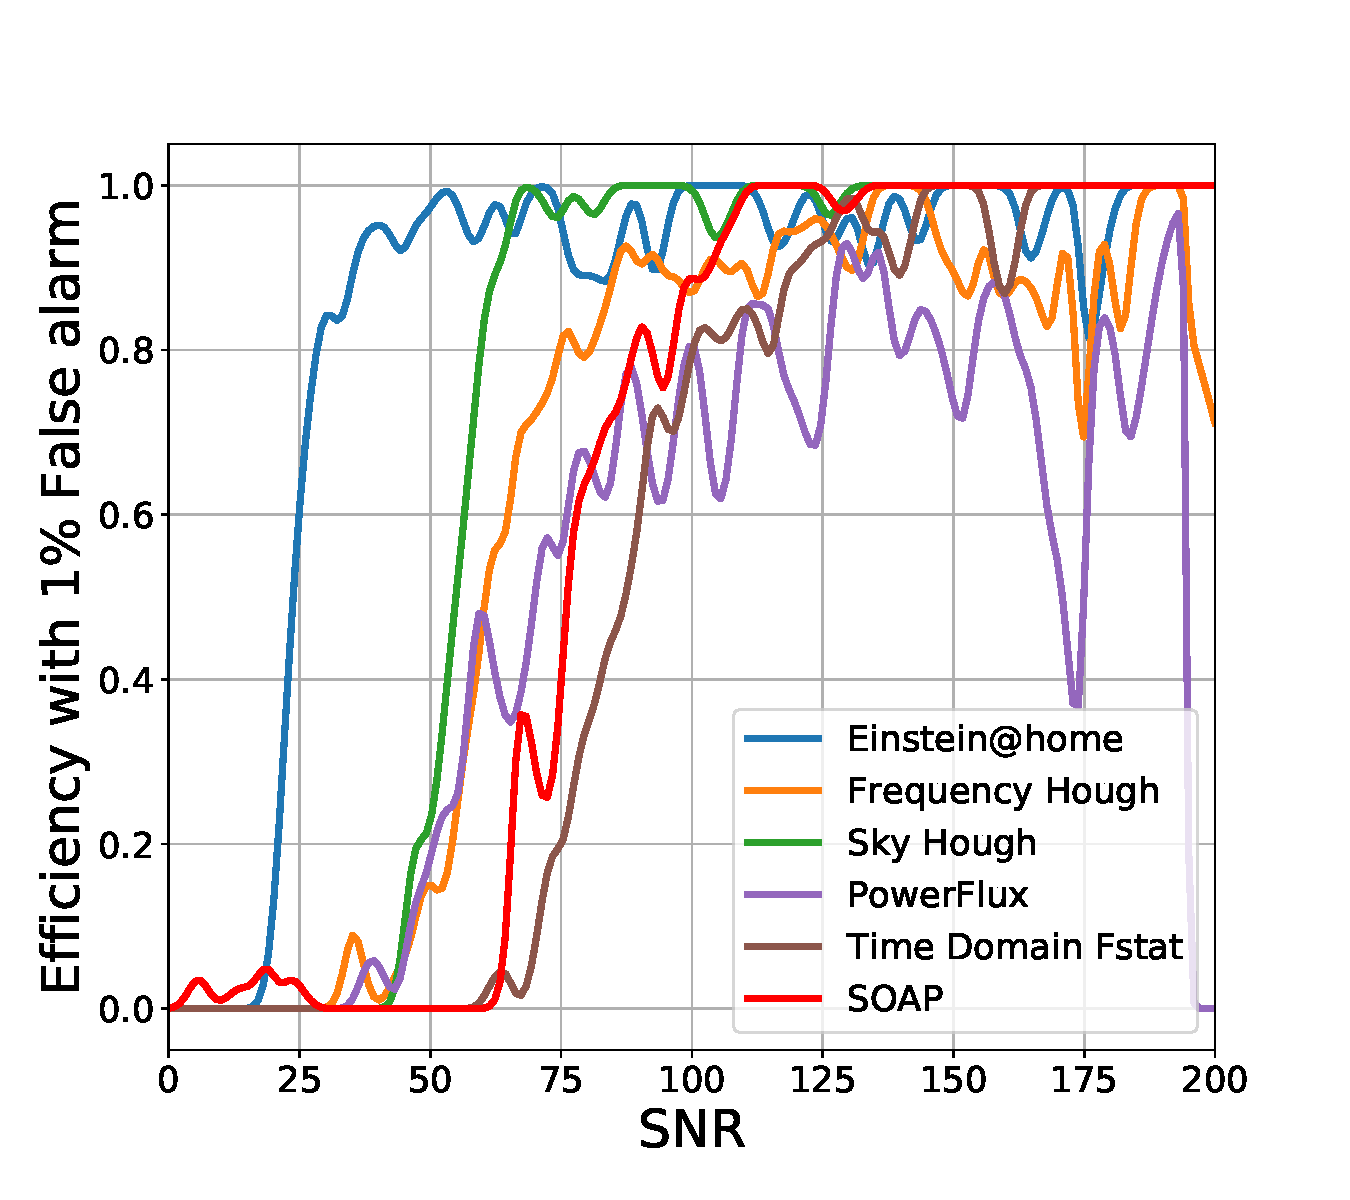
\includegraphics[width=\columnwidth]{C4_cnn/S6MDC_snr.pdf}
		\label{machine:results:snr_s6mdc}
	\end{subfigure}
\begin{subfigure}[h]{0.5\textwidth}
	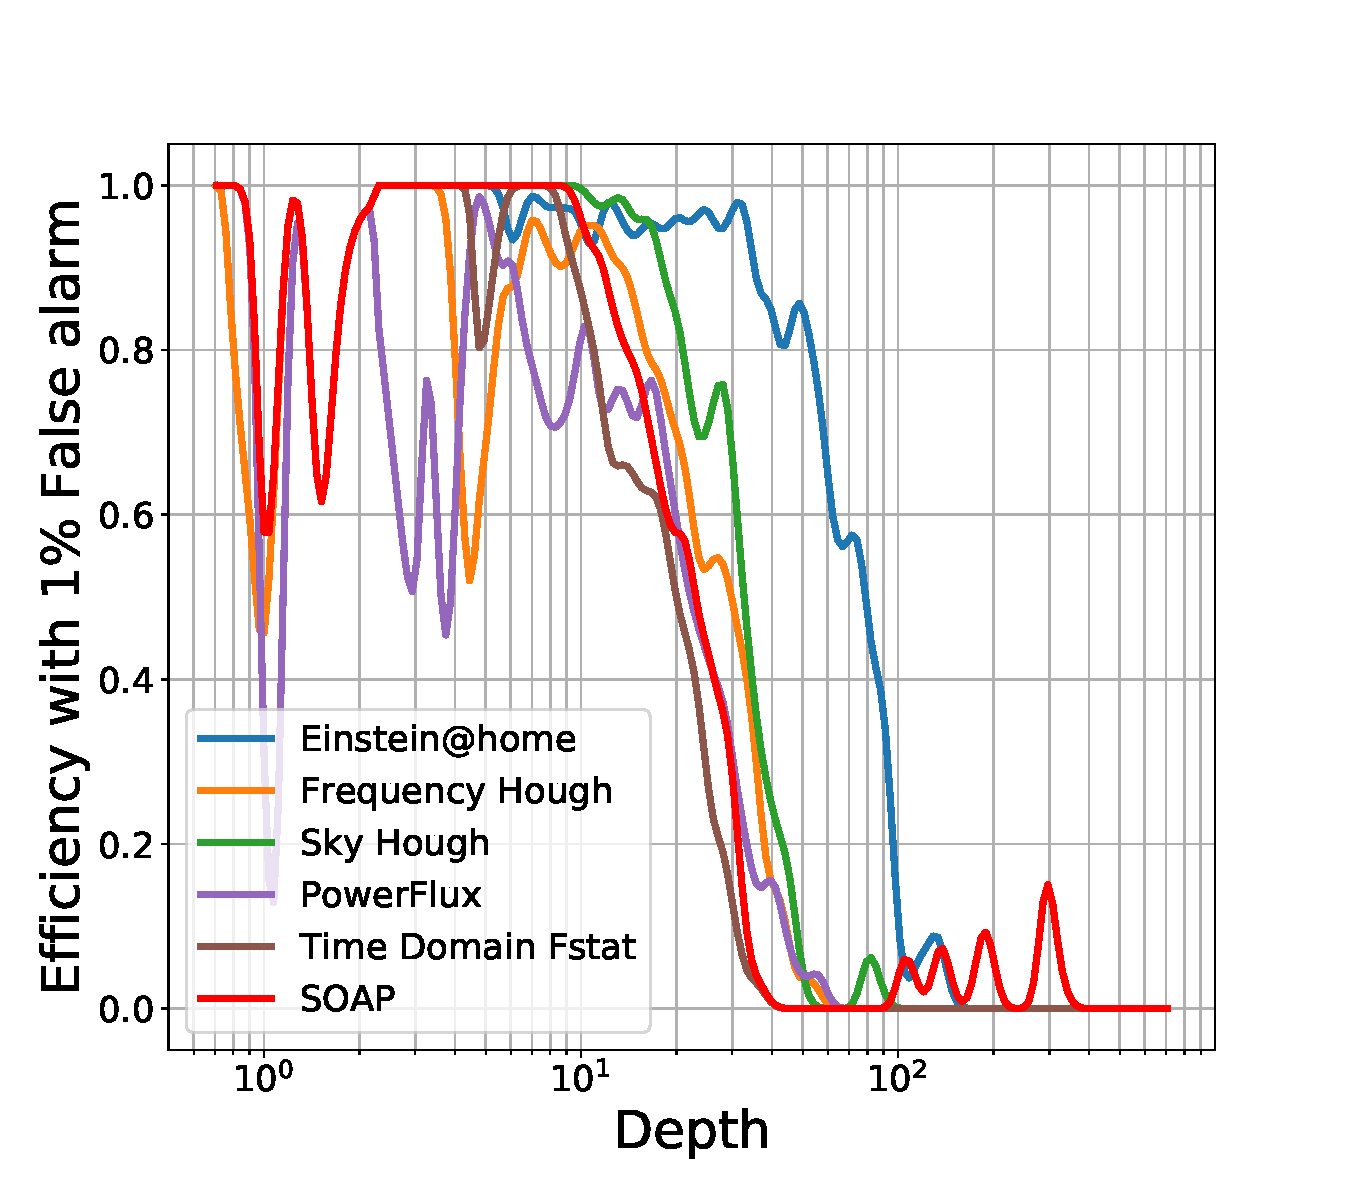
\includegraphics[width=\columnwidth]{C4_cnn/S6MDC_depth.pdf}
	\label{machine:results:mdccomp}
\end{subfigure}

	\caption{\label{machine:results:s6mdc} In the S6 \ac{MDC} \cite{walsh2016ComparisonMethods}, sensitivity curves were made for a set of \ac{CW} searches. 
		We have taken the list of detected pulsars for each search from this paper \cite{walsh2016ComparisonMethods} and replotted using the method in Sec.~\ref{sensitivity} to compare the sensitivities. 
		This is results for all pulsar injections in the 40-500 Hz band in the S6 \ac{MDC}.
		This shows how the SOAP search with a \ac{CNN} achieves a similar sensitivity some other \ac{CW} searches. 
	}
	
\end{figure}


\subsection{\label{results:timing} Computational time}

A key part of any \ac{CW} search is the computational time taken, the majority of the time for this search is used generating the appropriate data. 
For each section of the pipeline we have take the average total time for each job to complete, where each job runs on 2.0 Hz and it runs between 100 and 400 Hz. These are approximate timings taken for all the jobs to finish when run on CIT and can vary.

\begin{table}[h]
	%                     
	\centering                                                                                            
	\caption{\label{timing:table}Table shows the timings for each part of the search. These are approximate timings and vary when different amounts of data are input. This was run on data between 100-400 Hz.}
	
	%   
	\scalebox{0.8}{%
	\bgroup
	\def\arraystretch{1.5}
	\centering
	\begin{tabular}{c c c}
		\multicolumn{3}{c}{{\bf Generating data on CPU}}  \\
		\hline
		\hline
		& Time [hrs] & \\
		\hline
		Narrow-banding & $9$ &  \\
		\hline
		Training data& $239$ & \\
		\hline
		Test data& $75$ & \\
		\hline
		Search data& $40$ & \\
		\hline
		\hline
		\multicolumn{3}{c}{{\bf Training \acp{CNN} on GPU} }  \\
		\hline
		\hline
		& Training time [hrs] & Loading time [hrs]\\
		\hline
		Viterbi statistic & $0.03$ & $0.2$ \\
		\hline
		Viterbi map & $0.8$ & $0.7$ \\
		\hline
		spectrogram & $9$ & $1$\\
		\hline
		Viterbi map \\ + Viterbi statistic& $1$ &$0.7$ \\
		\hline
		Viterbi map \\ + spectrogram& $1.4$ & $1.6$\\
		\hline
		Viterbi map \\ + Viterbi statistic \\ + spectrogram& $1.5$ & $2$ \\
		\hline
		\hline
		\multicolumn{3}{c}{{\bf Testing \acp{CNN} on real data on GPU}}  \\
		\hline
		\hline
		& Testing [s] & Loading [s] \\
		\hline
		& $5$ & $60-160$ \\
		\hline
		\hline
	\end{tabular}
	\egroup
}
\end{table}

This gives the entire search including testing a total run time of $ \sim 386$ hours, however, the majority of the time is taken generating data which can be easily parallelised. 
Rather than taking hundreds of hours, the generating data sections takes $\mathcal{O}(1)$ hours in real time.


%%%%%
%%%%%
\section{\label{machine:cnn:sens_size} Sensitivity with the size of dataset}
%%%%%
%%%%%

When training a network, the general rule is the more data the better. 
This limits effects such as over-training mentioned in Sec.~\ref{machine:nn:training}.
To investigate how the sensitivity of the search changes with the number of training examples, the Viterbi map (vitmap) network in Sec.\ref{machine:results} was trained using a range of different training example numbers. 
These networks are then tested on the same dataset to see how they perform.
This was repeated for two data-sets: \ac{CW} simulations in Gaussian noise and simulations in \acp{LIGO} O1 data-set. 
For both of these cases six different networks were trained, these used 100, 500, 1000, 5000, 10000 and 15000 Viterbi maps as their training datasets.
Here the training data-sets are the same used as in Sec.~\ref{}.
These were then tested on the same data-sets in Sec.~\ref{}.

In the Gaussian noise case, the majority of the networks performed the same. 
This is with the exception of the network which was trained with 100 input Viterbi maps. 
The implication of this is that the information in the Viterbi maps is relatively easy to extract in this case. 
As the network is trying to distinguish Gaussian noise from a simulated \ac{CW} signal, one would expect this to be the easiest of all examples above to solve. \joe{dont like this explanation}

\begin{figure}[h]
	\begin{subfigure}[h]{0.5\textwidth}
		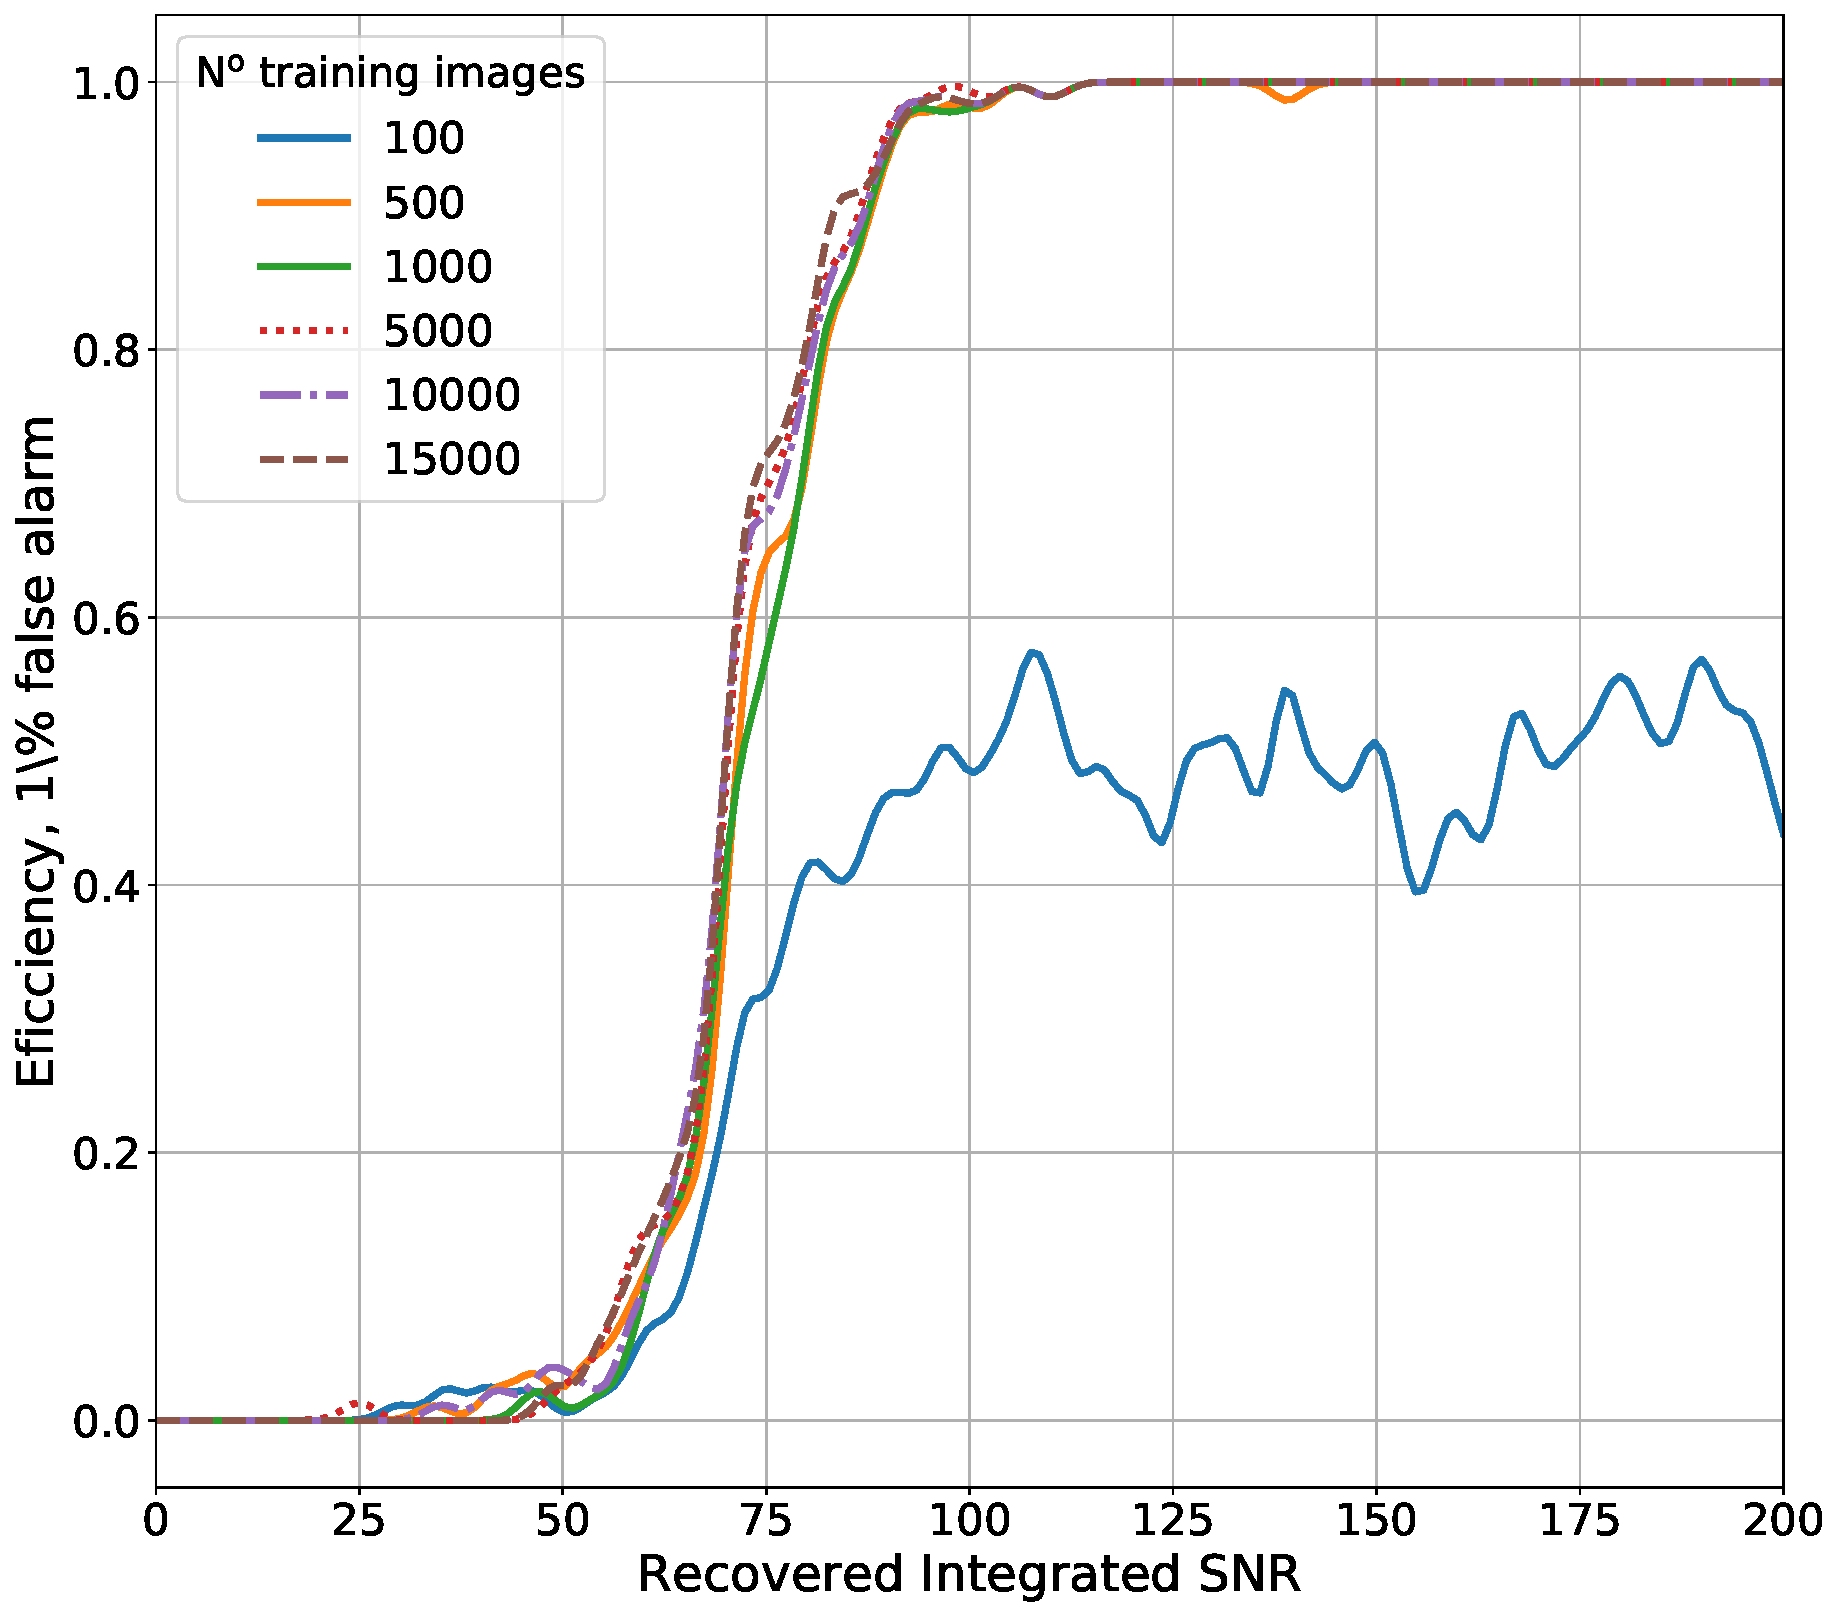
\includegraphics[width=\linewidth]{C4_cnn/gauss_sens_with_trainnum_eff.pdf}
		\caption{}
	\end{subfigure}
	\begin{subfigure}[h]{0.5\textwidth}
		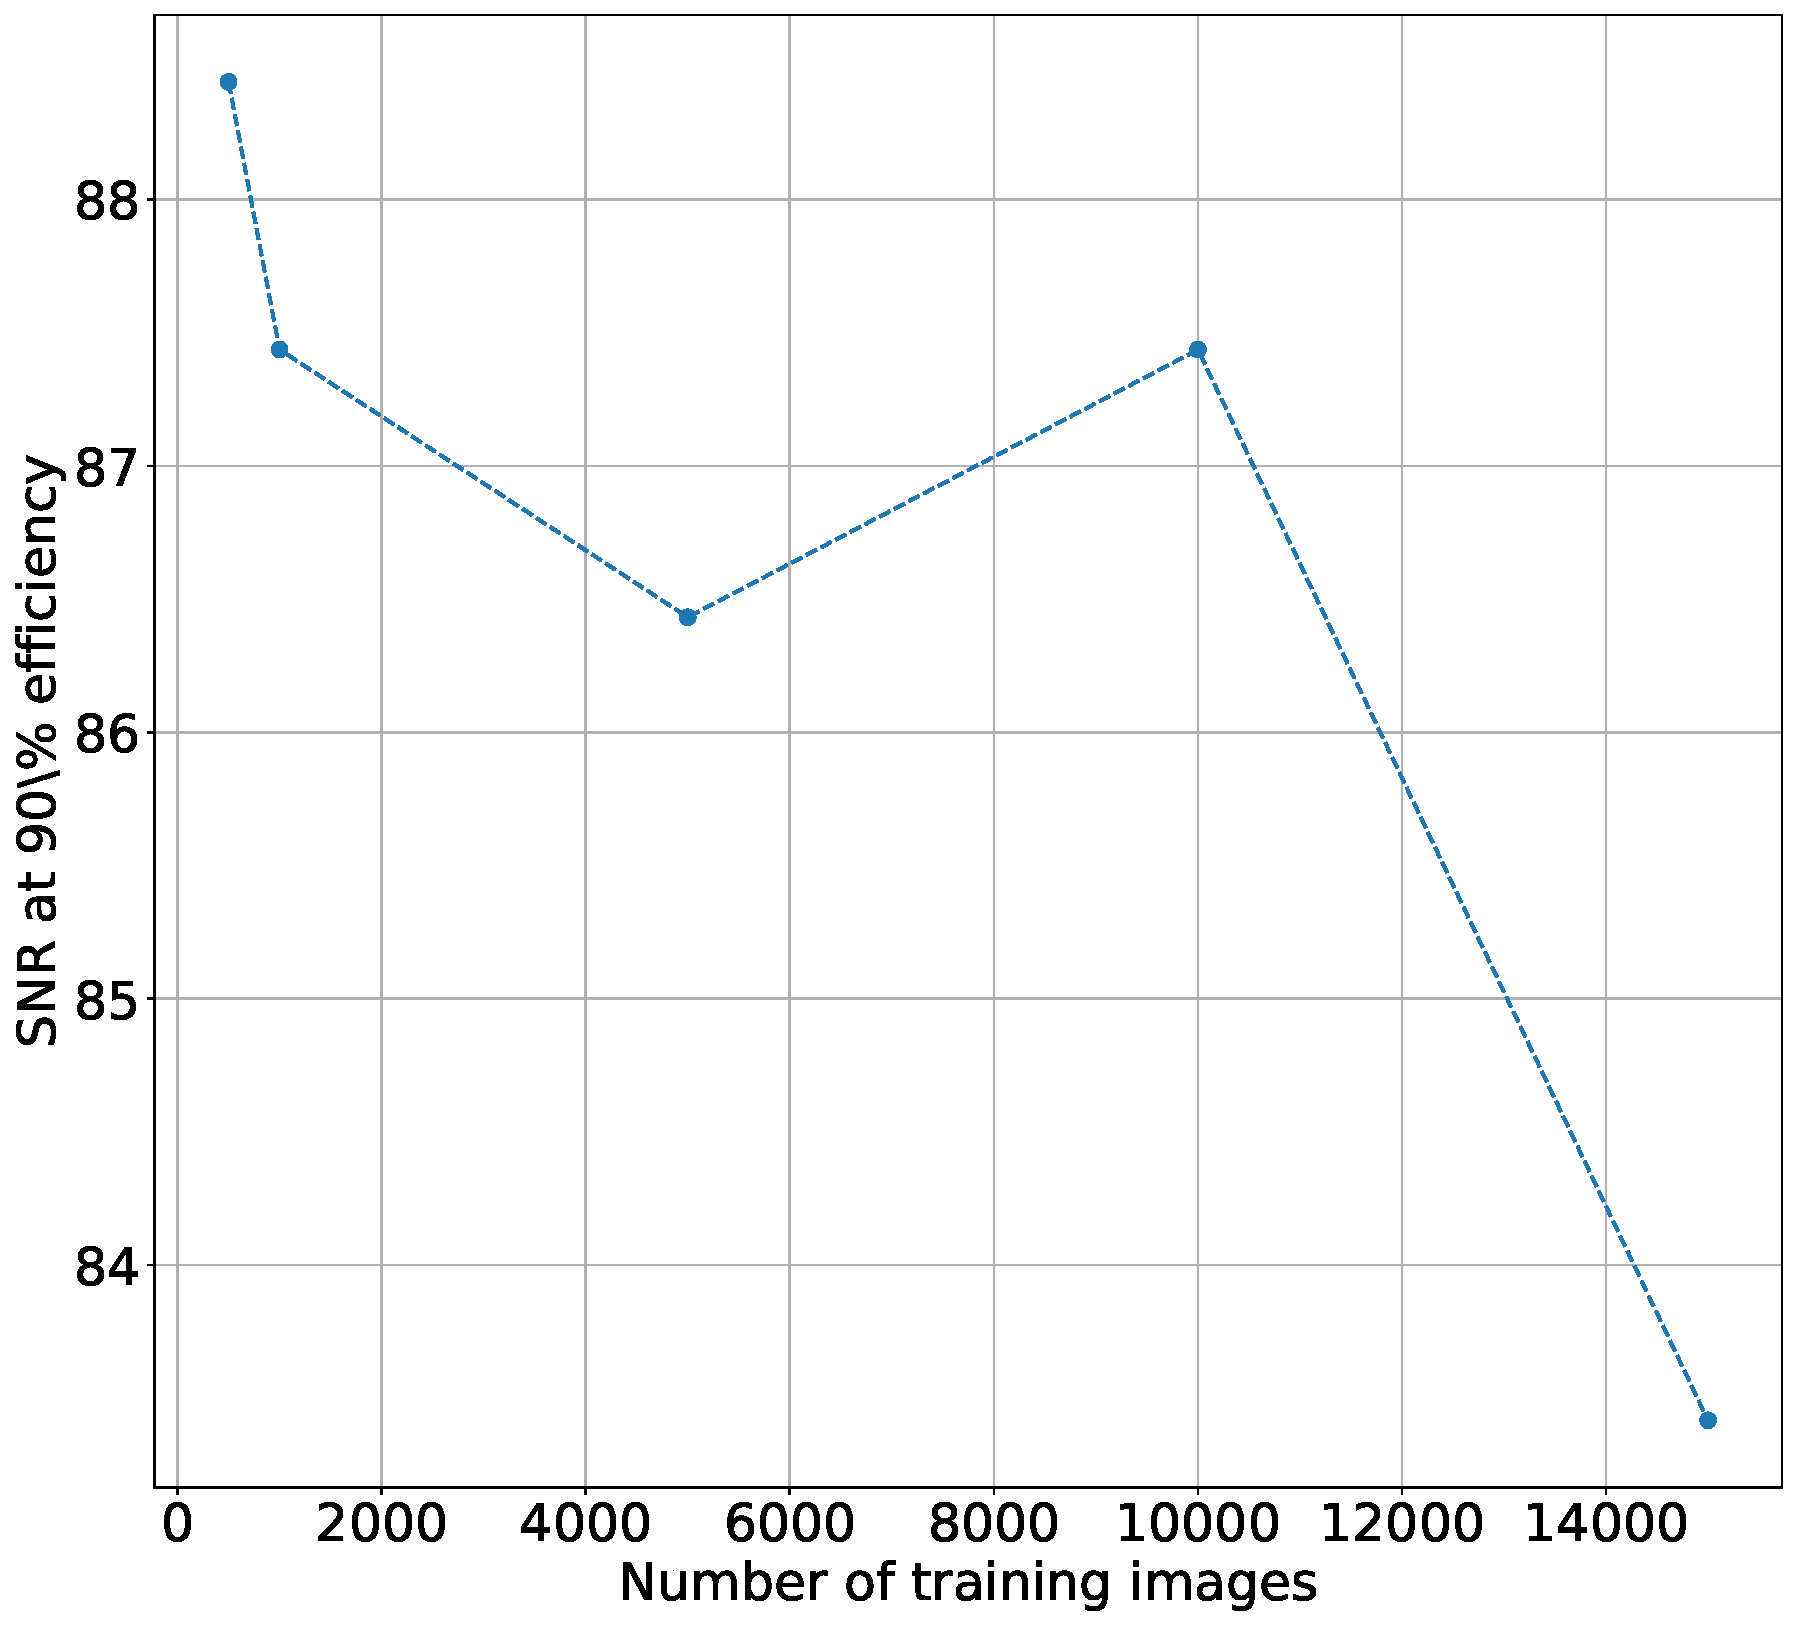
\includegraphics[width=\linewidth]{C4_cnn/gauss_sens_with_trainnum.pdf}
		\caption{}
	\end{subfigure}
	\caption{}
	\label{machine:cnn:sens_size:gauss_sens}
\end{figure}

When simulating signals in real O1 data, many of the sub-bands will contain instrumental lines. 
The noise class for the networks then contains many variations compared to the Gaussian noise case. 
This a harder challenge to the neural network by essentially increasing the size of the parameter space.
Because of this, one would expect the network to need many more training examples to be able to achieve a similar sensitivity to Gaussian noise.
In Fig.~\ref{machine:cnn:sens_size:o1_sens}, one can see that using 100 training examples is not enough and the network does not achieve any sensitivity at any \ac{SNR}.
The increase in training examples has a larger affect than in the Gaussian noise case. \joe{is that true}



\begin{figure}[h]
	\begin{subfigure}[h]{0.5\textwidth}
		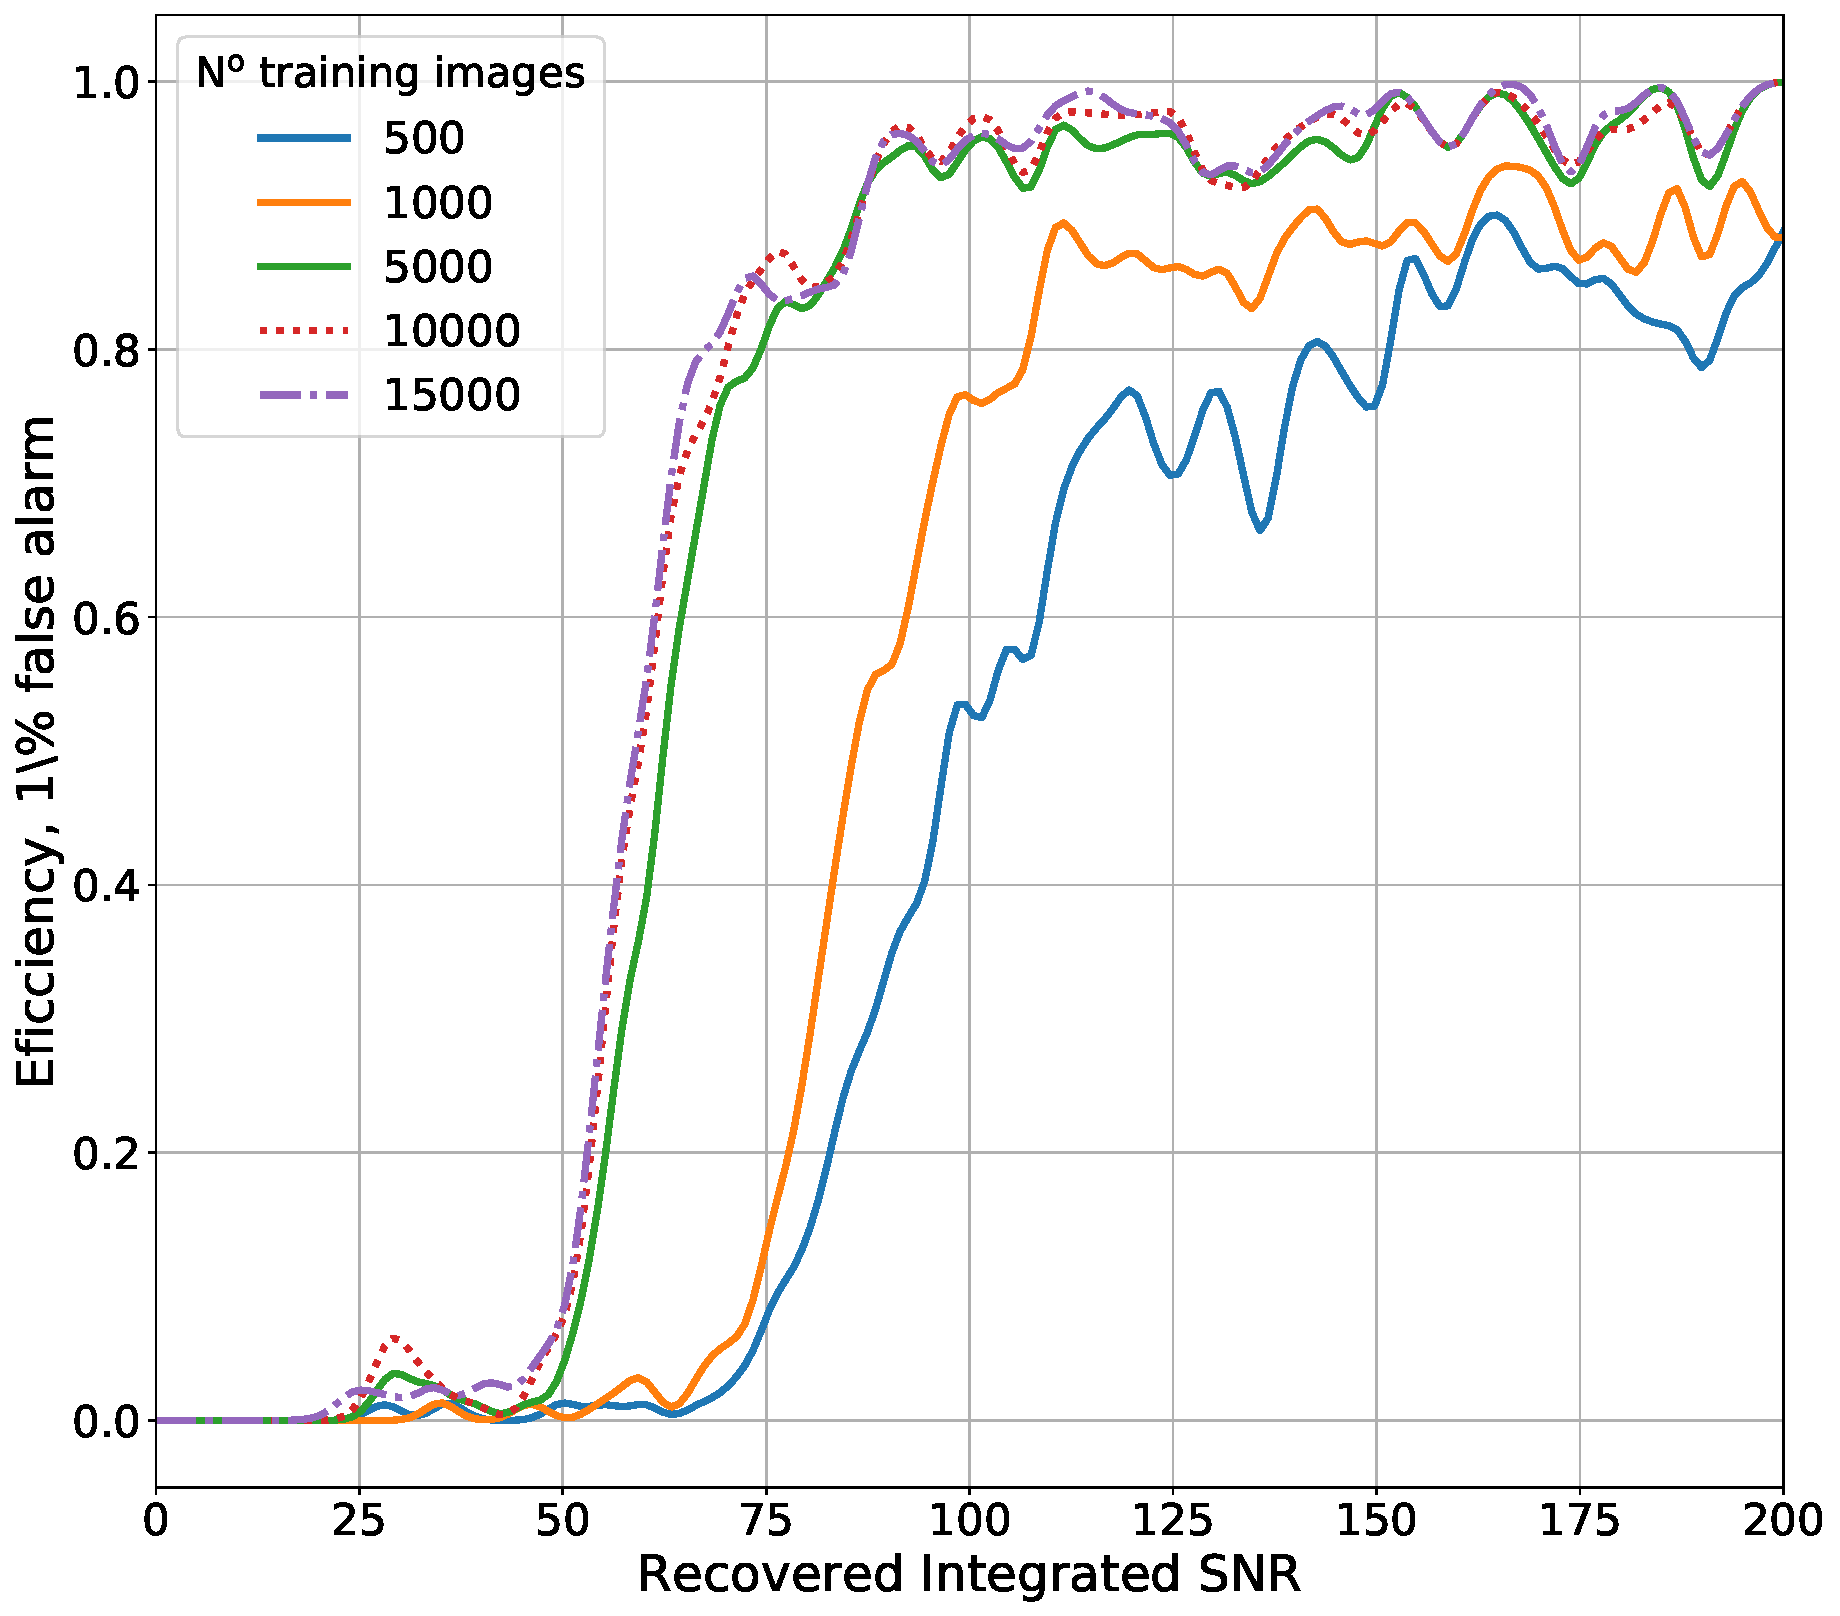
\includegraphics[width=\linewidth]{C4_cnn/o1_sens_with_trainnum_eff.pdf}
		\caption{}
	\end{subfigure}
	\begin{subfigure}[h]{0.5\textwidth}
		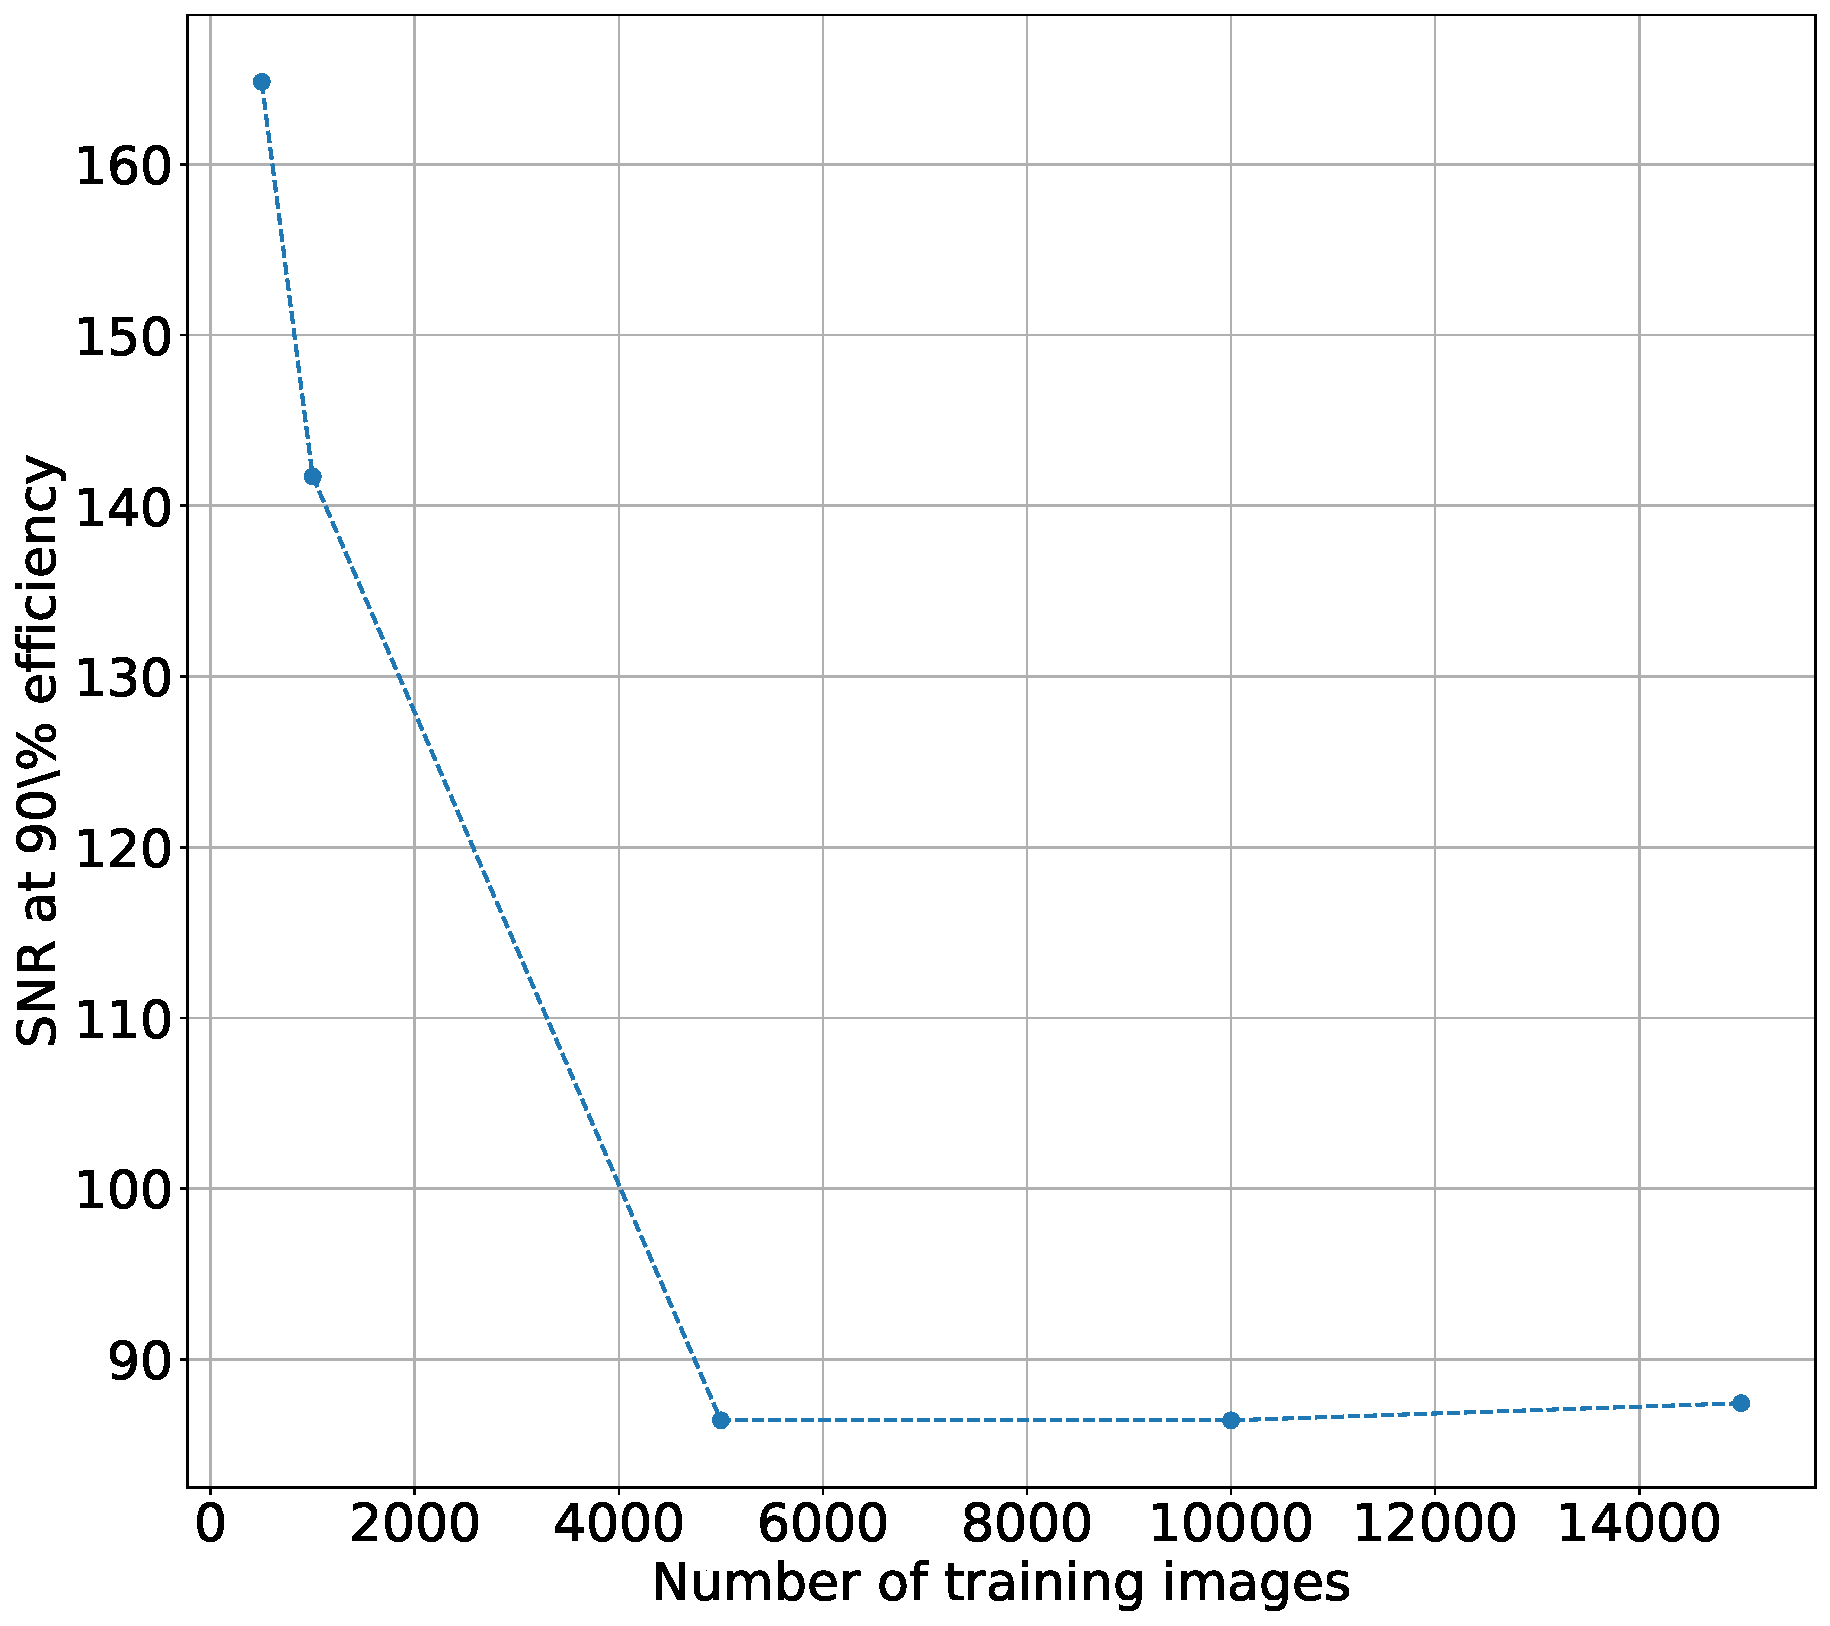
\includegraphics[width=\linewidth]{C4_cnn/o1_sens_with_trainnum.pdf}
		\caption{}
	\end{subfigure}
	\caption{}
	\label{machine:cnn:sens_size:o1_sens}
\end{figure}



%%%%%%%%%%%
%%%%%%%%%%%
\section{\label{cnn:networkvis}Network Visualisation}
%%%%%%%%%%%
%%%%%%%%%%%

Neural network are generally hard to visualise due to the large number or parameters in the network that have to be varied.
However, there are methods which can be used to see how input data is affected by the network.
This can be useful to see how the network performs when given certain types of data and gives some insight into how the networks work

In the examples above we use \acp{CNN}, the first few layers of this are build using convolutional filters.
The filters weights should ideally correspond to the shape of the feature which one wants to extract from the image. 
Generally this is only useful to picture at the first layer as the network can make subsequent layer and representations quite abstract.



\begin{figure}[h]
	\centering
	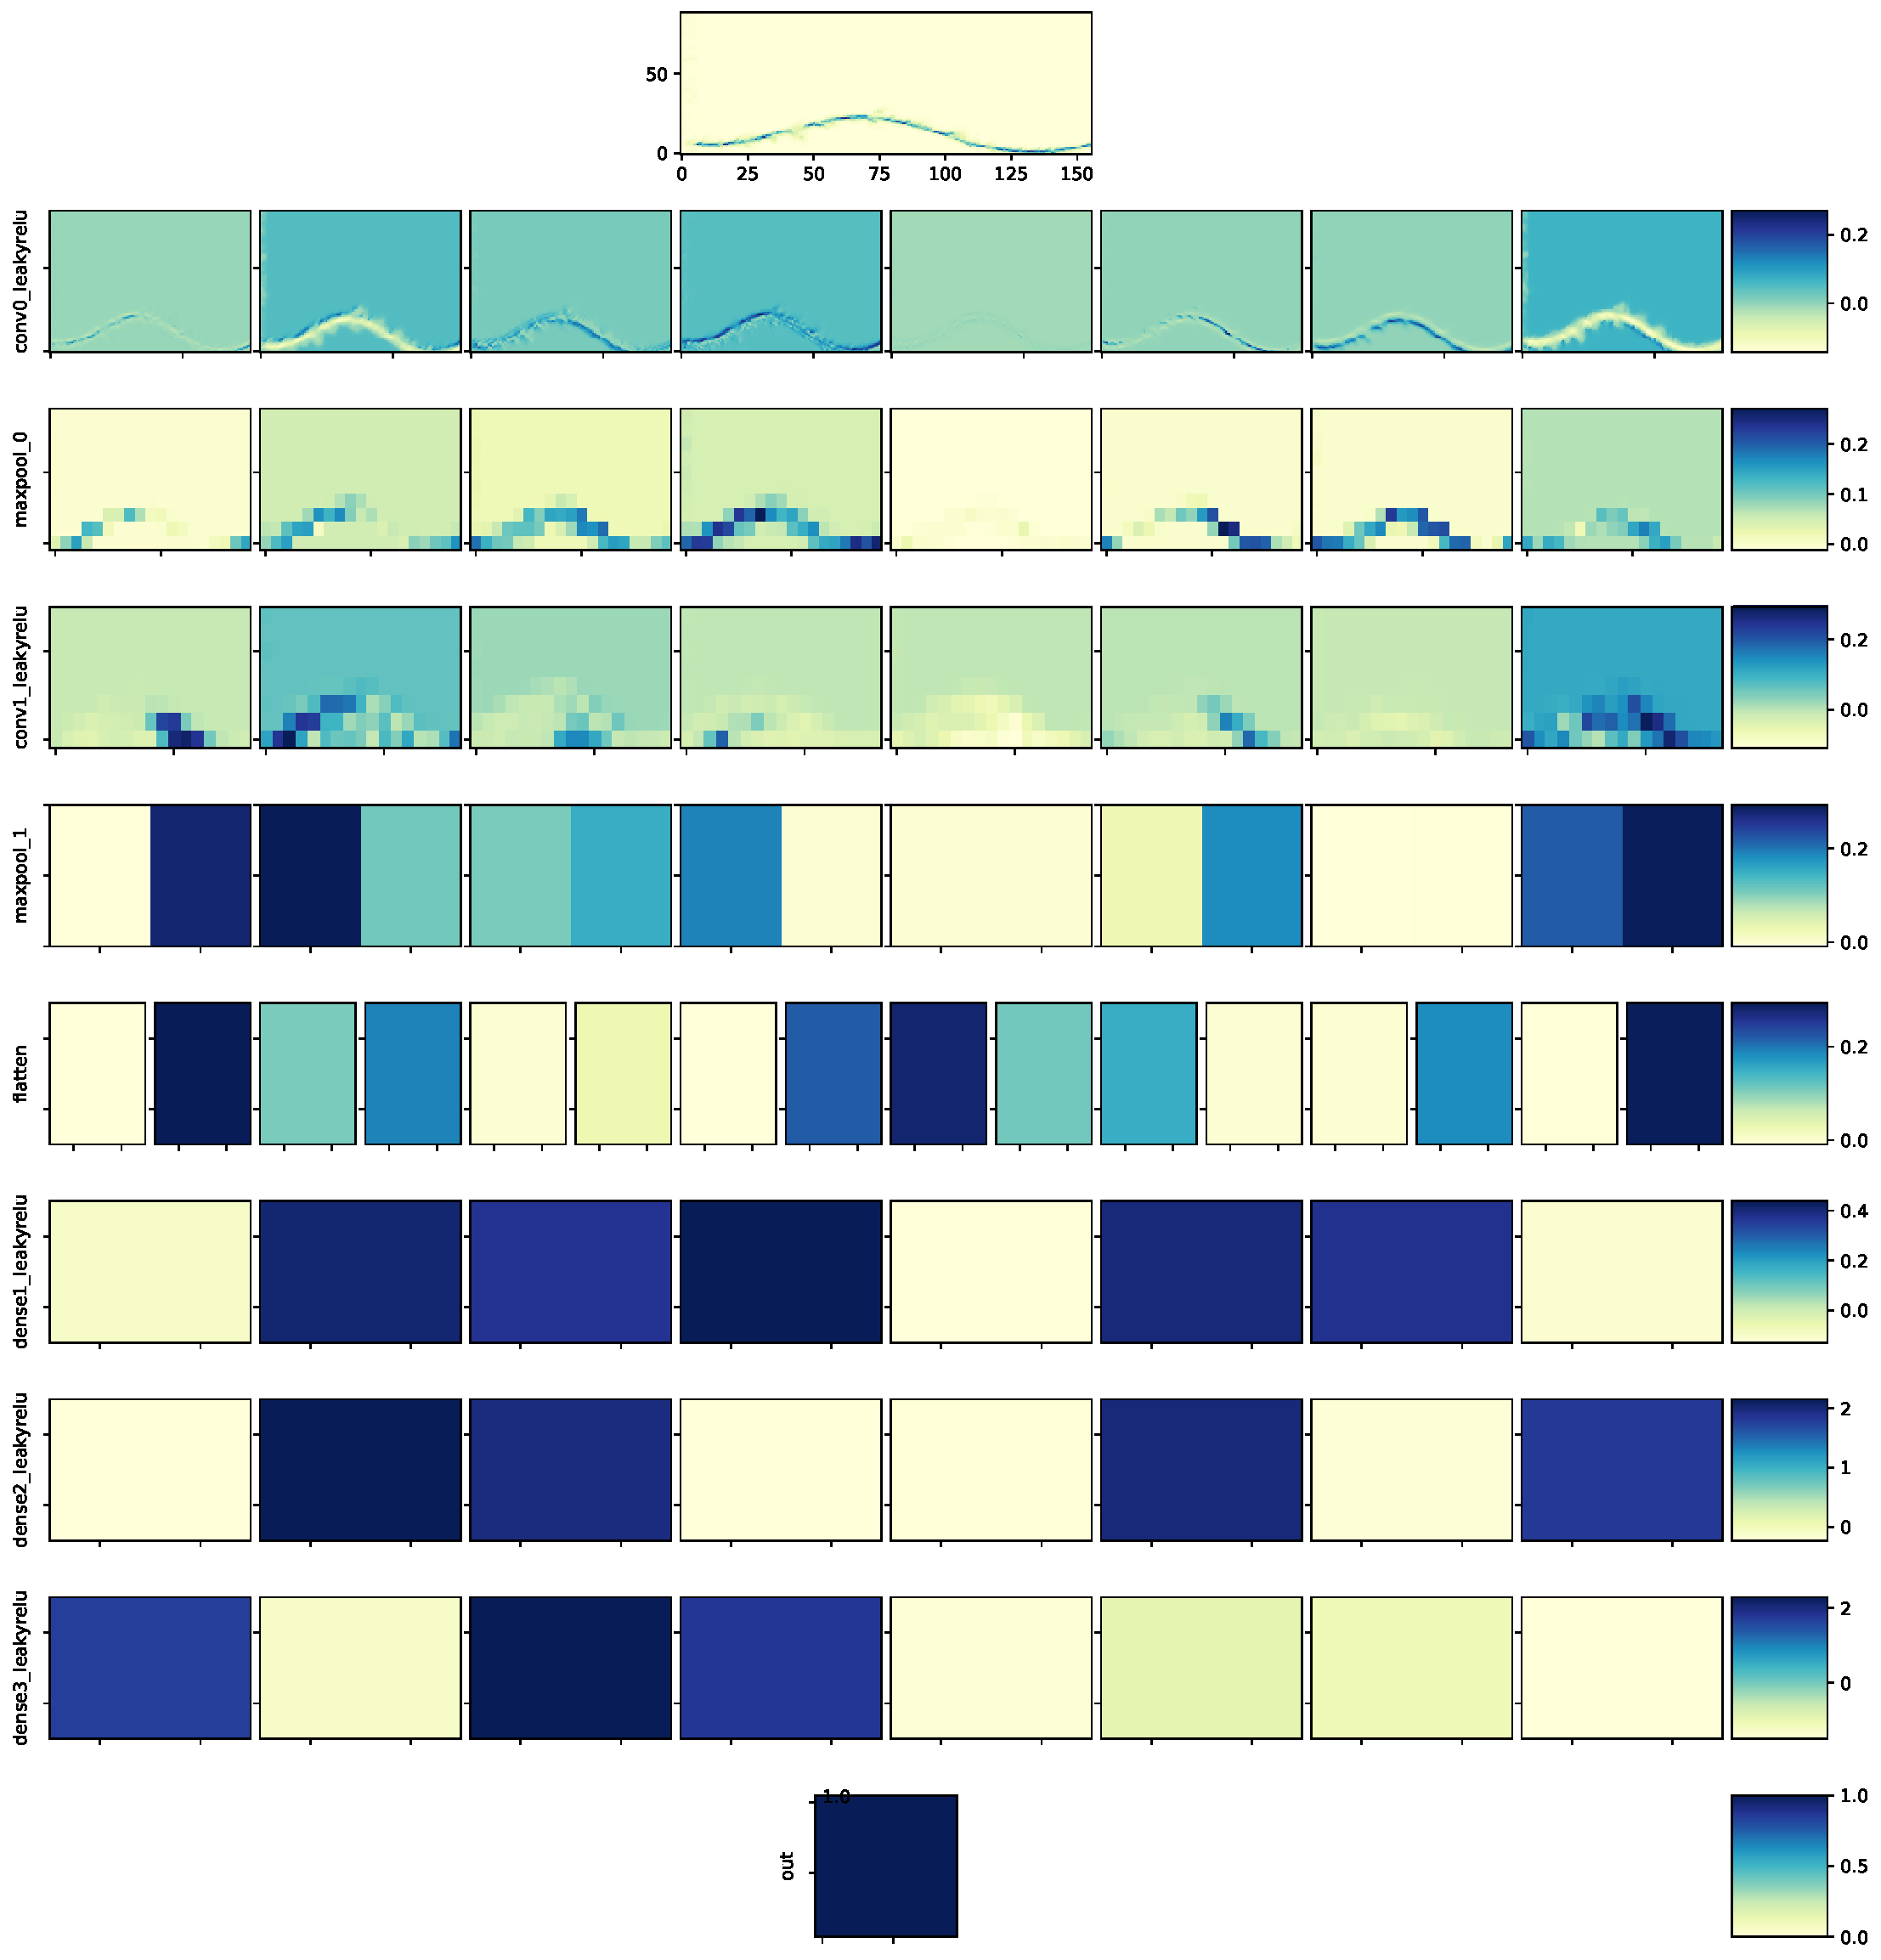
\includegraphics[width=\textwidth]{C4_cnn/vitmap_cnn_visualisation_signal.pdf}
	\caption{This shows a visualisation of the convolution neural network used for Viterbi maps above}
	\label{cnn:vis:vitmap:signal}
\end{figure}


%%%%%%%%%
%%%%%%%%
\section{Summary}
%%%%%%%%%
%%%%%%%%%

In this paper we summarise an extension of the SOAP algorithm which makes use of a \ac{CNN} to limit the effect of instrumental lines in a search for sources of continuous gravitational waves.
The SOAP search has a number of outputs for a given input spectrogram, where the main focus here is the Viterbi statistic and the Viterbi map. 
The Viterbi statistic has previously been used as a measure of whether there is a signal in a given frequency band, and the Viterbi maps are images which have the same shape as the input spectrogram, but gives a likelihood that there is a signal in a given location. 
The aim of the \ac{CNN} was to use the Viterbi maps and spectrograms as input images such that each frequency band can be classified to either having a signal or not. 
This would then remove then need to manually look through frequency bands and remove ones which are contaminated with non astrophysical features. 

We tested 6 separate \acp{CNN} which all take in different input data or different combinations of data as input. 
The three input data types are: the Viterbi statistic, the Viterbi map and the spectrograms which are summed and divided by a running median.
The aim of using different input data types is that each would provide a different piece of information than the others, this had the hope that the combinations of these should then increase our sensitivity. 
The tests found that the \ac{CNN} which uses the Viterbi map alone as input was more sensitive than any other which used a single data type as input. 
Each of the \acp{CNN} which used a combination of input data types had a similar sensitivity to the Viterbi map \ac{CNN}, therefore, it is assumed that the Viterbi map provides the most useful information when detecting a signal. 
Given that the main aim of this paper was to reduce the effect of instrumental lines on the SOAP search, in Gaussian noise data, the \ac{CNN} search should achieve a similar sensitivity to the Viterbi statistic alone. 
The tests in Gaussian noise with S6 gaps showed that at a 95 \% efficiency and a 1\% false alarm rate the Viterbi statistic and Viterbi map achieved a sensitivity of SNR 95 and 90 respectively. 
When the same test was run in real S6 data at a 95 \% efficiency and a 1\% false alarm rate the Viterbi statistic and Viterbi map achieved a sensitivity of SNR 300 and 120 respectively.
This demonstrates that the Viterbi map has a much larger effect when used on real data due to the presence of many instrumental lines within real data. 

These tests were once again repeated using a standard set of injections into S6 data such that a direct comparison can be made with other \ac{CW} search pipelines. 
At a 95 \% efficiency and a 1\% false alarm rate the Viterbi map \ac{CNN} achieved a sensitivity of \ac{SNR} $ \sim 90$ and sensitivity depth $\sim 14 \; \rm{Hz}^{-1/2}$ .
We have shown that the SOAP + \ac{CNN} approach can achieve a similar sensitivity to other semi-coherent \ac{CW} search algorithms but with a greatly reduced computational cost.

This search also offers a lot of flexibility in the signal type which can be searched, in the above examples the focus is on isolated neutron stars such that a comparison can be made to other \ac{CW} searches, however, this search is un-modelled. By changing the input parameters of the search, different signal types can be searched over, and in the future we aim to test its ability to identify more exotic sources of \ac{GW}. 
Further to this, we aim to make minor modifications to this pipeline such that some of the source parameters can be approximated. This should then return enough information to pass onto a more sensitive search for the signal. 


